\documentclass[english]{article}
\usepackage[title={Advanced Computer Architectures}, date={2022/2023}]{notestemplate}

\begin{document}

\makecover

\section*{Introduction}

This document contains the notes for the \textit{Advanced Computer Architectures} course, relative to the \textit{2021/2022} class of \textit{Computer Science and Engineering} held at \textit{Politecnico di Milano}.

\bigskip

\begin{itemize}
  \item Teacher: \textit{Donatella Sciuto}
  \item Support teacher: \textit{Davide Conficconi}
  \item Textbook: \textit{Hennessey and Patterson, Computer Architecture: A Quantitative Approach}
\end{itemize}

\bigskip

By comparing these notes with the material \textit{(slides, video lessons)} provided during the lectures, you will find a lot of discrepancies in the order in which they are represented.

This might look like a bizarre \textit{(if not completely stupid)} choice, but it has been deliberate as I have found the lessons quite confusing in their ordering and how each topic was introduced.
You will still find each of the topics explained during the lessons, including something more \textit{(sometimes)}.

\bigskip

If you find any errors and you are willing to contribute and fix them, feel free to send me a pull request on the GitHub repository found at \href{https://github.com/lorossi/advanced-computer-architectures-notes}{github.com/lorossi/advanced-computer-architectures-notes}.

\bigskip

A big thank you to everyone who helped me!

\clearpage

\section{Introduction to the Computer Architectures}

\subsection{Flynn Taxonomy}
\label{sec:flynn-taxonomy}

Created in \(1996\) and upgraded in \(1972\), it provides the first description of a computer.

\begin{itemize}
  \item \textit{SISD} - \textbf{single} instruction, \textbf{single} data
        \begin{itemize}
          \item \textbf{Sequential} programs
          \item \textbf{Serial} (non parallel) computer
          \item \textbf{Deterministic} execution
          \item Only \textbf{one instruction stream} is being executed at a time
        \end{itemize}
  \item \textit{MISD} - \textbf{multiple} instructions, \textbf{single} data
        \begin{itemize}
          \item Multiple processors working in \textbf{parallel} on the same data
          \item \textbf{Fail safe} due to high redundancy
          \item The same algorithm is programmed and implemented in different ways, so if one fails the other is still able to compute the result
          \item \textbf{No practical market configuration}
        \end{itemize}
  \item \textit{SIMD} - \textbf{single} instruction, \textbf{multiple} data
        \begin{itemize}
          \item Each processor receives \textbf{different data} and performs the \textbf{same operations} on it
          \item Used in fields where a single operation must be performed in many different pieces of information \textit{(like in image processing)}
          \item Each instructions is executed in \textbf{synchronous} way on the same data
          \item Best suited for specialized problems characterized by a high degree of regularity, such as graphics or images processing
          \item \textbf{Data level parallelism} \textit{(DLP)}
        \end{itemize}
  \item \textit{MIMD} - \textbf{multiple} instructions, \textbf{multiple} data
        \begin{itemize}
          \item \textbf{Array of processors} in parallel, each of them executing its instructions
          \item Execution can be \textbf{asynchronous} or \textbf{synchronous}, \textbf{deterministic} or \textbf{non-deterministic}
          \item The \textbf{most common} type of parallel computer
        \end{itemize}
\end{itemize}

\bigskip
\textit{MIMD} an \textit{SIMD} architectures will be further explained in Sections~\ref{sec:mimd}~and~\ref{sec:simd}.
An illustration of the different architectures is displayed in Figure~\ref{fig:flynn-taxonomy}.

\begin{figure}[htbp]
  \bigskip
  \centering
  \tikzfig[1]{image-1.tikz}
  \caption{Flynn Taxonomy}
  \label{fig:flynn-taxonomy}
  \bigskip
\end{figure}

\clearpage

\subsection{Hardware parallelism}

There are different types of hardware parallelisms:

\begin{itemize}
  \item \textbf{Instruction Level parallelism} - \textit{(ILP)}
        \begin{itemize}
          \item Exploits data level parallelism at modest level through \textbf{compiler techniques} such as pipelining and at medium levels using speculation
        \end{itemize}
  \item \textbf{Vector Architectures} and \textbf{Graphic Processor Units}
        \begin{itemize}
          \item Exploit data level parallelism by applying a single instruction to a \textbf{collection of data} in parallel
        \end{itemize}
  \item \textbf{Thread level parallelism} - \textit{(TLP)}
        \begin{itemize}
          \item Exploits either data level parallelism or task level parallelism in a coupled hardware model that allows \textbf{interaction among threads}
        \end{itemize}
  \item \textbf{Request level parallelism}
        \begin{itemize}
          \item Exploits parallelism among largely decoupled tasks specified by the programmer or the OS
        \end{itemize}
\end{itemize}

Nowadays, heterogeneous systems \textit{(systems that utilize more than one type of parallelism)} are commonly used among all commercial devices.

\clearpage

\section{Performance and cost}

There are multiple types \textit{(classes)} of computers, each with different needs:
the performance measurement is not the same for each of them.
\textit{Price, computing speed, power consumption} can be metrics to measure the performance of a computer.

Programming has become so complicated that it's not possible to balance all the constraints manually;
while the computational power has grown bigger than ever before, energy consumption is now a sensible constraint.

The computer engineering methodology is therefore described as:

\begin{figure}[htbp]
  \bigskip
  \centering
  \begin{minipage}[h]{0.495\textwidth}
    \centering
    \tikzfig[1]{image-2.tikz}
  \end{minipage}
  \begin{minipage}[h]{0.495\textwidth}
    \begin{enumerate}
      \item \label{enum:methodology-start} \textit{evaluate} system by bottlenecks
      \item \textit{simulate} new designs and organizations
      \item \textit{implement} next generation systems
      \item \textit{repeat}
    \end{enumerate}
  \end{minipage}
  \caption{Computer engineering methodology}
  \label{fig:computer-engineering-methodology}
  \bigskip
\end{figure}

There are more constraints not contained in this model, such as technology trends.

\bigskip
When one computer is faster than another, what quality is being addressed?
The answer is not always the same, and it depends on the application;
different solutions may consider different metrics, such as
speed of execution, power consumption, cost, etc.

The picked qualities may change according to the use case or the user themself,
but 2 metrics are normally used:

\begin{enumerate}
  \item \textbf{Elapsed time}
        \begin{itemize}
          \item \(\texttt{execution time} = \texttt{time end} - \texttt{time start}\)
          \item More relevant for system user
        \end{itemize}
  \item \textbf{Completion rate}
        \begin{itemize}
          \item \(\texttt{completion rate} = \texttt{number of jobs} \div \texttt{elapsed time}\)
          \item More relevant for the system designer
        \end{itemize}
\end{enumerate}

\subsection{Response time vs throughput}

Is it true that
\(\texttt{throughput} = {1} \div { \texttt{average response time}}\)?
The answer can be given only if it's clear if there's an overlap between core operations.

If there is, then 
\begin{equation}
  \texttt{throughput} > {1} \div {\texttt{average response time}} 
\end{equation}
With pipelining, \textbf{execution time} of a single instruction is \textbf{increased} while the \textbf{average throughput} is \textbf{decreased}.

\subsection{Factors affecting performance}

A few of the factors affecting the performance are:

\begin{itemize}
  \item Algorithm complexity and data sets
  \item Compiler
  \item Instructions set
  \item Available operations
  \item Operating systems
  \item Clock rate
  \item Memory system performance
  \item I/O system performance and overhead
        \begin{itemize}
          \item this it's the least optimizable factor, the main focus is then to optimize all the others
        \end{itemize}
\end{itemize}

\bigskip
The locution \textbf{\(X\) is \(n\) times faster than \(Y\)} can be expressed as:

\begin{gather*}
  \dfrac{ExTime\ (Y)}{ExTime\ (X)}  = \dfrac{Performance\ (X)}{Performance\ (Y)} = Speedup\ (X, Y) \\
  Performance(X) = \dfrac{1}{ExTime\ (x)}
\end{gather*}

So, in order to optimize a system, it's necessary to focus on common sense (a \textit{sadly} valuable quality).
While making a design trade-off one must favour the frequent case over the infrequent one.

\textit{For example}:
\begin{itemize}
  \item Instructions fetch and decode unit is used more frequently than the multiplier
        \begin{itemize}
          \item it makes sense to optimize \textbf{instructions fetch unit} first
        \end{itemize}
  \item If database server has \(50\) disks processor, storage dependability is more important than system dependability
        \begin{itemize}
          \item it makes sense to optimize \textbf{storage dependability} first
        \end{itemize}
\end{itemize}

\subsubsection{Amdahl's law}

As seen before, the speedup due to the enhancement \(E\) is:
\[ Speedup\ (E)  = \dfrac{ExTime\ w/o\ E}{ExTime\ w/\ E} = \dfrac{Performance\ w/\ E}{Performance\ w/o\ E} \]

Suppose that enhancement \(E\) accelerates a fraction \(F\) of the task by a factor \(S\) and the remainder of the task is unaffected.
Amdahl's law states that:
\begin{gather*}
  ExTime_{new} = ExTime_{old} \times \left[\left(1 - F\right) + \dfrac{F}{S}\right] \\
  Speedup = \dfrac{ExTime_{old}}{ExTime_{new}} = \dfrac{1}{(1 - F) + \sfrac{F}{S}} = \dfrac{S}{S - SF + F}
\end{gather*}

\paragraph{Corollary}

The best possible outcome of the \textit{Amdahl's law} is:
\[ Speedup = \dfrac{1}{1 - F} \]

\indentquote{If an enhancement is only usable for a fraction of the task, we can't speed up the task by more than the reciprocal of \(1\) minus the fraction}

The \textit{Amdahl's law} expresses the law of diminishing returns.
It serves as a guide to how much an enhancement will improve performance and how to distribute resources to improve the cost-over-performance ratio.

\subsubsection{\textit{CPU} time}

\textbf{CPU time} is determined by:

\begin{itemize}
  \item \textbf{Instruction Count} - \textit{IC}:
        \begin{itemize}
          \item The number of executed instructions, not the size of static code
          \item Determined by multiple \textit{factors, including algorithm, compiler, ISA}
        \end{itemize}
  \item \textbf{Cycles per instructions} - \textit{CPI}:
        \begin{itemize}
          \item Determined by \textit{ISA} and \textit{CPU} organization
          \item Overlap among instructions reduces this term
          \item The \textit{CPI} relative to a process \texttt{P} is calculated as:
                \[
                   CPI(P) = \dfrac{\texttt{\# of clock cycles to execute P}}{\texttt{number of instructions}} 
                \]
        \end{itemize}
  \item \textbf{Time per cycle} - \textit{TC}:
        \begin{itemize}
          \item It's determined by technology, organization and circuit design
        \end{itemize}
\end{itemize}

\bigskip
Then, \textit{CPU} time can be calculated as:
\[ CPU_{time} = T_{clock} \cdot CPI \cdot N_{inst} = \dfrac{CPI \cdot N_{inst}}{f} \]
Note that the \textit{CPI} can vary among instructions because each step of the pipeline might take different amounts of time.
The factors that can influence the \textit{CPU} time are shown in Table~\ref{tab:relation-factor-CPU-time}.

\begin{table}[htbp]
  \centering
  \begin{tabular}{r|c|c|c}
                             & \textit{IC} & \textit{CPI} & \textit{TC} \\ \hline
    \textit{Program}         & \xmark      &              &             \\
    \textit{Compiler}        & \xmark      & (\xmark)     &             \\
    \textit{Instruction set} & \xmark      & \xmark       &             \\
    \textit{Organization}    &             & \xmark       & \xmark      \\
    \textit{Technology}      &             &              & \xmark      \\
  \end{tabular}
  \caption{Relation between factors and \textit{CPU} time}
  \label{tab:relation-factor-CPU-time}
\end{table}

\paragraph{\textit{CPU} time and cache}

To improve the \textit{CPU} time, an \textbf{instruction cache} can be used.
Using a more realistic model, while calculating \textit{CPU} time, one must also account for:

\begin{itemize}
  \item The \textbf{execution} \textit{CPI} - \(\text{CPI}_\text{EXE}\)
  \item The \textbf{miss penalty} - \(\text{MISS}_P\)
  \item The \textbf{miss rate} - \(\text{MISS}_R\)
  \item The memory \textbf{references} - \(\text{MEM}\)
\end{itemize}

Then the \(\text{CPI}_{\text{CACHE}}\) can be calculated as:
\[ \text{CPI}_{\text{CACHE}} = \text{CPI}_\text{EXE} + \text{MISS}_P \cdot  \text{MISS}_R \cdot \text{MEM} \]

\subsubsection{Other metrics}

There are other metrics to measure the performance of a \textit{CPU}:

\begin{itemize}
  \item \textit{MIPS} - millions of instructions per second
        \[ MIPS = \dfrac{\texttt{number of instructions}}{\texttt{execution time} \cdot 10^6} = \dfrac{\texttt{clock frequency}}{\texttt{CPI} \cdot 10^6} \]
        \begin{itemize}
          \item the higher the \textit{MIPS}, the faster the machine
        \end{itemize}
  \item \textit{Execution time}
        \[ T_{execution} = \dfrac{\texttt{instruction count}}{\texttt{MIPS} \cdot 10^6} \]
  \item \textit{MFLOPS} - floating point operations in program
        \begin{itemize}
          \item assumes that floating points operations are independent of the compiler and ISA
          \item it's not always safe, because of:
                \begin{itemize}
                  \item missing instructions \textit{(e.g. FP divide, square root, sin, cos, \dots)}
                  \item optimizing compilers
                \end{itemize}
        \end{itemize}
\end{itemize}

Furthermore, the execution time is compared against test programs that:

\begin{itemize}
  \item Are chosen to measure performance defined by some groups
  \item Are available to the community
  \item Run on machines whose performance is well-known and documented
  \item Can compare to reports on other machines
  \item Are representative
\end{itemize}

\subsection{Averaging metrics}

The simplest approach to summarizing relative performance is to use the total execution time of the \(n\) programs;
however, this generalization does account for the different durations of the benchmarking programs.

The \textbf{\(3\) different approaches} using means to average a metric are described in Table~\ref{tab:mean-approaches}.

\begin{table}[htbp]
  \centering
  \begin{tabular}{c|c}
    \textit{metric} & \textit{type of mean} \\ \hline
    times           & arithmetic            \\
    rates           & harmonic              \\
    execution time  & geometric             \\
  \end{tabular}
  \caption{Mean approaches}
  \label{tab:mean-approaches}
\end{table}

\clearpage

\section{Multithreading and Multiprocessors}

\textbf{Thread (filo):} instruction stream with own PC and data
\begin{itemize}
  \item thread may be a process part of a parallel
  program of multiple processes, or it may
  be an independent program
  \item Each thread has all the state (instructions,
  data, PC, register state, and so on)
  necessary to allow it to execute
  \item Threads share single address space   
\end{itemize}

\subsection{Why multithreading?}

Why is multithreading needed?

\begin{itemize}
  \item \textit{80's}: expansions of superscalar processors
        \begin{itemize}
          \item In the '80s, people were writing languages in high-level programming languages
          \item Since compiler optimization was not good enough, it was needed to improve the software translations by making \textit{CPU} instructions that were more similar to high-level instructions
          \item In order to improve performances, the \textbf{pipeline} was introduced
                \begin{itemize}
                  \item it sends \textbf{more than one instructions at a time}
                  \item more instructions completed in the same clock cycle
                  \item it's kind of a hardware-level implicit parallelism
                \end{itemize}
        \end{itemize}
  \item \textit{90's}: decreasing returns on investments
        \begin{itemize}
          \item Since all the parallelism was implemented by the hardware \textit{(or, at most, the compiler)}, there was no effective way to manually handle the performance
          \item There were many different issues:
                \begin{itemize}
                  \item issue from \(2\) to \(6\) ways, issue out of order, branch prediction, all lowering from \(1\) \textit{CPI} to \(0.5\) \textit{CPI}
                  \item performance below expectations
                  \item these performance issues led to delayed and cancelled projects
                \end{itemize}
          \item All the previous improvements were due to the shrinking size of the transistors, which was slowly speeding down
                \begin{itemize}
                  \item the number of transistors followed Moore's law, doubling each \(18\) to \(24\) months
                  \item the frequency and the performance per core were not, due to interferences and energy problems
                \end{itemize}
        \end{itemize}
  \item \textit{2000}: beginning of the multi-core era
        \begin{itemize}
          \item Since increasing the \textit{CPU} frequency could not be achieved anymore, the only solution left was to increase the number of threads in every processor
          \item This implied that there was a need of introducing a software way to handle the parallelism, in harmony with an enhanced hardware
        \end{itemize}
\end{itemize}

\bigskip
Motivations for the paradigm change:

\begin{itemize}
  \item Moderns processors \textbf{fail to utilize execution resources} well enough
        \begin{itemize}
          \item There's no single culprit:
                \begin{itemize}[label=\xmarkthin]
                  \item \textit{memory conflicts}
                  \item \textit{control hazards}
                  \item \textit{branch misprediction}
                  \item \textit{cache miss}
                  \item \ldots
                \end{itemize}
          \item All those problems are correlated and there's no way of solving one of them without affecting all the others
          \item There's the need for a general latency-tolerance approach that can hide all sources of latency
                \begin{itemize}[label=\cmarkthin]
                  \item a solution is found in \textbf{parallel programming}
                \end{itemize}
        \end{itemize}
\end{itemize}

\subsubsection{Parallel Programming}

\textbf{Multithreading:} something not related to underlying architecture. It concern SO.

Explicit parallelism implies structuring the applications into concurrent and communicating tasks.
Operating systems offer systems to implement such features: \textbf{threads} and \textbf{processes}:
\begin{itemize}
  \item process: program in execution. A process doesn't share information directly
  \item thread: instruction stream with own PC and data. lightweight process. (unità atomica di un processo che deve essere eseguito insieme). 
\end{itemize}


The multitasking is implemented differently based on the characteristics of the \textit{CPU}:

\begin{itemize}
  \item \textbf{Single} core
  \item \textbf{Single} core with \textbf{multithreading} support
  \item \textbf{Multi} core
\end{itemize}

In multithreading, multiple threads share the function units of one processor via overlapping.
The processor must duplicate the independent state of each thread:

\begin{itemize}
  \item Separate copy of the \textbf{register files}
  \item Separate \textbf{\texttt{PC}}
  \item Separate\textbf{ page table}
\end{itemize}

\begin{figure}[htbp]
  \bigskip
  \centering
  \tikzfig{image-3.tikz}
  \caption{Multiplicity of processes and threads (in one core (probably))}
  \label{fig:multiplicity-of-processes-and-threads}
  \bigskip
\end{figure}

The memory is shared via the virtual memory mechanisms, which already support multi processes.
Finally, the hardware must be ready for a fast thread switch: it must be faster than a full process switch \textit{(which is in the order of hundreds to thousands of clocks)}.

There are \(2\) apparent solutions:

\begin{enumerate}
  \item \textbf{Fine grained} multi-threading
        \begin{itemize}
          \item Switches from one thread to another at each instruction by \textbf{taking turns}
                \begin{itemize}
                  \item the switch happens when one thread stalls
                \end{itemize}
          \item The executions of more threads is \textbf{interleaved}
          \item The \textit{CPU} must be able to change thread at \textbf{every clock cycle}
          \item For \(n\) processes, each gets \(\sfrac{1}{n}\) of \textit{CPU} time
                \begin{itemize}
                  \item \(n\) times the original resources are needed
                \end{itemize}
        \end{itemize}
  \item \textbf{Coarse grained} multithreading
        \begin{itemize}
          \item Switching from one thread to another occurs only when there are long \textbf{stalls} in the active process
          \item The interested threads \textbf{share many resources}
          \item The switching from one thread to the other requires \textbf{different clock cycles} to save the context
        \end{itemize}
\end{enumerate}

\bigskip

\textbf{Disadvantages} of multithreading:
\begin{itemize}[label=\xmarkthin]
  \item For short stalls it \textbf{does not reduce the throughput loss}
  \item The \textit{CPU} starts the execution of instructions that belongs to a \textbf{single thread}
  \item When there is one stall it is necessary to \textbf{empty the pipeline} before starting the new thread
\end{itemize}

\textbf{Advantages} of multithreading:
\begin{itemize}[label=\cmarkthin]
  \item In normal conditions \textbf{the single thread is not slowed down}
\end{itemize}

\begin{figure}[htbp]
  \bigskip
  \centering
  \tikzfig[1]{image-4.tikz}
  \caption{\centering Comparison between fine and coarse multithreading. Each column shows the evolution of \(2\) different processes spread on \(4\) different threads over a set amount of time.
    A filled square illustrates a thread occupied by a process, while the empty ones represent an empty \texttt{(idle)} thread.}
  \label{fig:multithreading-fine-coarse-comparison}
  \bigskip
\end{figure}

\paragraph{Thread Level Parallelism - \textit{TLP}}

\begin{itemize}
  \item \textbf{Thread level parallelism}, simultaneous multithreading
        \begin{itemize}
          \item Uses the resources of \textbf{one superscalar processor} to exploit simultaneously \textit{ILP} and \textit{TLP}
          \item A \textit{CPU} today has \textbf{more functional resources} than what one thread can in fact use
          \item Simultaneously \textbf{schedule instructions} for execution from all threads
        \end{itemize}
  \item A \textit{CPU} that can handle these needs must be built
        \begin{itemize}
          \item A \textbf{large set of registers} is needed, allowing multiple processes to operate on different data on the same registers
          \item \textbf{Mapping table for registers} is needed in order to tell each process where to write data
          \item Each processor can manage a \textbf{set amount of threads}
        \end{itemize}
  \item This is the most \textbf{flexible} way to manage multithreading but it requires more \textbf{complex hardware}
\end{itemize}
\bigskip

Comparison between many multithreading paradigms is shown in Figure~\ref{fig:multithreading-comparison}.

\begin{figure}[htbp]
  \bigskip
  \centering
  \tikzfig[0.85]{image-5.tikz}
  \caption{\centering Multithreading comparison. Each column shows the evolution of \(5\) different processes spread on \(4\) different threads over a set amount of time.
    A filled square illustrates a thread occupied by a process, while the empty ones represent an empty \texttt{(idle)} thread.}
  \label{fig:multithreading-comparison}
  \bigskip
\end{figure}

\subsubsection{Further improvements}

It's difficult to increase the performance and clock frequency of the single core.
The longest pipeline stage can be split into multiple smaller stages, allowing higher throughput.

This concept is called \textbf{deep pipeline} and has a few drawbacks:

\begin{itemize}
  \item \textbf{Heat dissipation} problems due to the increased number of components
  \item More stages imply \textbf{more faults} since sequential instructions are likely related
  \item \textbf{Transmissions delay} in wires start to get relevant
  \item \textbf{Harder design} and verifications by the hardware developers
\end{itemize}

\subsection{Parallel Architectures}

A \textbf{parallel computer} is a collection of processing elements that cooperate and communicate to solve large problems rapidly.

The aim is to replicate processors to add performance and not design a single faster processor.
The parallel architecture extends traditional computer architecture with a communication architecture.
This solution needs:

\begin{itemize}
  \item \textbf{Abstractions} for HW/SW interface
  \item \textbf{Different structures} to realize abstractions easily
\end{itemize}

Refer to Flynn Taxonomy \textit{(Section~\ref{sec:flynn-taxonomy})} for more details about these architectures.

\subsection{\textit{SIMD} architecture}

The characteristics of the \textit{SIMD} architectures \textit{(Single Instruction Multiple Data)} are:

\begin{itemize}
  \item \textbf{Same instruction} executed by \textbf{multiple processors} using different data streams
  \item Each processor has its data memory
  \item \textbf{Single instruction memory} and \textbf{single control processor} to fetch and dispatch instructions
  \item Processors are typically \textbf{special purpose}
  \item A \textbf{simple} programming model
\end{itemize}

The programming model features synchronized units with a single program counter, while each unit has its own addressing registers to use different data addresses.

\bigskip
Motivations for \textit{SIMD}:

\begin{itemize}
  \item The \textbf{cost} of the control unit is \textbf{shared} between all execution units
  \item Only\textbf{ one copy of the code} in execution is necessary
  \item All the computation is \textbf{fully synchronized}
\end{itemize}

In real life:

\begin{itemize}
  \item \textit{SIMD} architectures are a \textbf{mix} of \textit{SISD} and \textit{SIMD}
  \item A host computer executes \textbf{sequential operations}
  \item \textit{SIMD} instructions sent to all the execution units
        \begin{itemize}
          \item each of them has its own memory and registers
          \item an interconnection network is needed to exchange data
        \end{itemize}
\end{itemize}

\bigskip
\textit{SIMD} architectures will be explored in depth in Section~\ref{sec:simd}.

\begin{figure}[htbp]
  \bigskip
  \centering
  \tikzfig[1]{image-6.tikz}
  \caption{\textit{SIMD} architecture}
  \label{fig:simd-architecture}
  \bigskip
\end{figure}

\subsection{\textit{MIMD} architecture}

\textit{MIMD} architectures are flexible as they can function as:

\begin{itemize}
  \item \textbf{Single user} machines for high performance on one application
  \item Multi programmed multiprocessors running many tasks \textbf{simultaneously}
  \item Some combinations of the two aforementioned functions
\end{itemize}

They can also be built starting from standard CPUs.

\bigskip
Each processor fetches its own instructions and operates on its own data;
processors are often off-the-shelf microprocessors, with the upside of being able to build a scalable architecture and having a high cost-performance ratio.

In order to fully exploit a \textit{MIMD} with \(n\) processors, there must be:

\begin{itemize}
  \item At least \(n\) \textbf{threads} or \textbf{processes}  to execute
        \begin{itemize}
          \item those independent threads are typically identified by the programmer or created by the compiler
        \end{itemize}
  \item \textbf{Thread level parallelism} - \textit{TLP}
        \begin{itemize}
          \item parallelism is identified by the software \textit{(and not by hardware like in superscalar CPUs)}
        \end{itemize}
\end{itemize}

\textit{MIMD} machines can be characterized in \(2\) classes, depending on the number of processors involved:

\begin{itemize}
  \item \textbf{Centralized} shared-memory architectures
        \begin{itemize}
          \item At most a few dozen processors chips \textit{(less than \(100\) cores)}
          \item Large caches, single memory multiple banks
          \item This kind of structures is often \textbf{symmetric multiprocessors (SMP)} and the style of architecture is called \textbf{Uniform Memory Access (UMA)}
        \end{itemize}
  \item \textbf{Distributed} memory architectures
        \begin{itemize}
          \item Supports \textbf{large processor count}
          \item Requires \textbf{high bandwidth} interconnection
          \item It has the disadvantage of a high volume of data communication between processors
        \end{itemize}
\end{itemize}

\bigskip
\textit{MIMD} architectures will be explored in depth in Section~\ref{sec:mimd}.

\clearpage

\section{Pipeline recap}

The pipeline \textit{CPI} \textit{(clocks per instruction)} can be calculated taking account of:

\begin{itemize}
  \item \textbf{Ideal} pipeline \textit{CPI}
        \begin{itemize}
          \item measure of the maximum performance attainable by the implementation
        \end{itemize}
  \item \textbf{Structural stalls}
        \begin{itemize}
          \item due to the inability of the \textit{HW} to support this combination of instructions
          \item can be solved with more \textit{HW} resources
        \end{itemize}
  \item \textbf{Data hazards}
        \begin{itemize}
          \item the current instruction depends on the result of a prior instruction still in the pipeline
          \item can be solved with \textit{forwarding} or \textit{compiler scheduling}
        \end{itemize}
  \item \textbf{Control hazards}
        \begin{itemize}
          \item caused by delay between the \texttt{IF} and the decisions about changes in control flow \textit{(branches, jumps, executions)}
          \item can be solved with \textit{early evaluation, delayed branch, predictors}
        \end{itemize}
\end{itemize}

\begin{equation}
  \text{Pipeline CPI} = \text{Ideal pipeline CPI} + \text{Structural Stalls} + \text{Data Hazard Stalls} + \text{Control Stalls}  
\end{equation}

\smallskip
The main features of the pipeline are:
\begin{itemize}
  \item \textbf{Higher throughput} for the entire workload
  \item Pipeline rate is limited by the \textbf{slowest} pipeline stage
  \item Multiple tasks operate \textbf{simultaneously}
  \item It \textbf{exploits parallelism} among instructions
  \item Time needed to \textit{"fill"} and \textit{"empty"} the pipeline reduces speedup
\end{itemize}

\subsection{Stages in \textit{MIPS} pipeline}

The \(5\) stages in the \textit{MIPS} pipeline are:

\begin{enumerate}
  \item \textbf{Fetch} - \texttt{IF}
        \begin{itemize}[label=\(\rightarrow\)]
          \item Instruction fetch from memory
        \end{itemize}
  \item \textbf{Decode} - \texttt{ID}
        \begin{itemize}[label=\(\rightarrow\)]
          \item Instruction decode and register read
        \end{itemize}
  \item \textbf{Execute} - \texttt{EX}
        \begin{itemize}[label=\(\rightarrow\)]
          \item Execute operation or calculate the address
        \end{itemize}
  \item \textbf{Memory access} - \texttt{ME}
        \begin{itemize}[label=\(\rightarrow\)]
          \item Access memory operand
        \end{itemize}
  \item \textbf{Write back} - \texttt{WB}
        \begin{itemize}[label=\(\rightarrow\)]
          \item Write the result back to register
        \end{itemize}
\end{enumerate}

Each instruction is executed after the previous one has completed its first stage, and so on.
When the pipeline is filled, five different activities are running at once.
Instructions are passed from one unit to the next through a storage buffer.
As each instruction progresses through the pipeline, all the information needed by the stages downstream must be passed along.

The stages are usually represented in Figure~\ref{fig:mips-pipeline-stages}.

\begin{figure}[htbp]
  \bigskip
  \centering
  \tikzfig[1.5]{image-7.tikz}
  \caption{Stages in \textit{MIPS} pipelines}
  \label{fig:mips-pipeline-stages}
  \bigskip
\end{figure}

\newpage

\subsection{Pipeline hazards}
\label{sec:pipeline-hazards}

An \textbf{hazard} is a fault in a pipeline.
A hazard is created whenever there is a dependence between instructions that are close enough such that the overlap introduced by pipelining would change the order of access to the operands involved in said dependence.
It prevents the next instruction in the pipeline from executing during its designated clock cycle, reducing the performance from the ideal speedup.

\smallskip

There are \(3\) classes of hazards:
\begin{enumerate}
  \item \textbf{Structural} hazards, due to attempting to use the same resource from different instructions at the same time
  \item \textbf{Data} hazards \textit{stalls}, due to attempting to use a result before it is ready
        \begin{itemize}
          \item \textit{Read after write} - \textit{RAW}
                \begin{itemize}[label=\(\rightarrow\)]
                  \item the instruction tries to read a source register before it is written by a previous instruction
                  \item it's also called \textit{dependence} by compilers
                  \item caused by an actual need for communication
                \end{itemize}
          \item \textit{Write after read} - \textit{WAR}
                \begin{itemize}[label=\(\rightarrow\)]
                  \item the instruction tries to write a destination register before it is read by a previous instruction
                  \item it's also called \textit{anti dependence} by compilers
                  \item caused by the reuse of the same register for different purposes
                \end{itemize}
          \item \textit{Write after write} - \textit{WAW}
                \begin{itemize}[label=\(\rightarrow\)]
                  \item the instruction tries to write before it is written by a previous instruction
                  \item it's also called \textit{output dependence} by compilers
                  \item caused by the reuse of the same register for different purposes
                \end{itemize}
        \end{itemize}
  \item \textbf{Control} hazards \textit{stalls}, due to the request of deciding on the next instruction to execute before the condition itself is evaluated
\end{enumerate}

\medskip
\textit{Data stalls may occur with instructions such as}:
\begin{itemize}
  \item \textit{RAW} stall:
        \begin{verbatim}
    r3 := (r1) op (r2)
    r5 := (r3) op (r4)  // r3 has not been written yet\end{verbatim}
  \item \textit{WAR} stall:
        \begin{verbatim}
    r3 := (r1) op (r2)
    r1 := (r4) op (r5)  // r1 has not been read yet \end{verbatim}
  \item \textit{WAW}  \textit{stall}:
        \begin{verbatim}
    r3 := (r1) op (r2)
    r3 := (r6) op (r7) // r3 has not been written yet \end{verbatim}
\end{itemize}



\subsubsection{Solutions to data hazards}

Hazards limit performance:
\begin{itemize}
  \item Structural: need more HW resources
  \item Data: need forwarding, compiler scheduling
  \item Control: early evaluation \& PC, delayed branch, predictors   
\end{itemize}

\begin{remarks}
  Increasing length of pipe increases impact of hazards  
\end{remarks}

\begin{remarks}
  Pipelining helps instruction bandwidth, not latency  
\end{remarks}



There are many ways in which data hazards can be solved, such as:

\begin{itemize}
  \item \textbf{Compilation} techniques
        \begin{itemize}
          \item \textbf{Insertion of \texttt{nop}} instructions
          \item \textbf{Instructions scheduling}
                \begin{itemize}
                  \item the compiler tries to avoid that correlating instructions are too close
                  \item it tries to insert independent instructions among correlated ones
                  \item when it can't, it inserts \texttt{nop} operations
                \end{itemize}
        \end{itemize}
  \item \textbf{Hardware} techniques
        \begin{itemize}
          \item \textbf{Insertion} on \textit{bubbles} or \textit{stalls} in the pipeline
          \item Data \textbf{forwarding} (bypassing)
        \end{itemize}
\end{itemize}

Both the compilation and the hardware techniques will be analyzed in depth in Section~\ref{sec:strategies-to-support-ilp}.

\begin{remarks} 
  \textbf{Problem with Floating point operation} \hfill \break
  \textit{ADDD, SUBD, MULTD, DIVD} are floating pointing poin operation:
  \begin{itemize}
    \item Floating point operation are not commutative ($A+B \ne B+A$), due to approximation
    \item They take much more clock cycle than interger operation
    \item They use different type of data (integer and floating point)
  \end{itemize}

  $\rightarrow$ we need general purpose (integer) registers and floating point registers. 
\end{remarks}

\medskip

What about mixing Integer and Floating point operations?

\newpage

\subsection{Complex in-order pipeline}

While using floating points operations, a few questions might arise:

\indentquote{What happens, architecture-wise, when mixing integer and floating point operations? How are different registers handled? How can \textit{GPRs (general purpose registers)} and \textit{FPRs (floating point registers)} be matched?}

\begin{figure}[htbp]
  %\smallskip
  \centering
  \tikzfig[1]{image-8.tikz}
  \caption{Complex-in order pipeline}
  \label{fig:complex-in-order-pipeline}
  %\smallskip
\end{figure}

The pipeline is now constituted by \(6\) stages, normally represented as in Figure~\ref{fig:mips-pipeline-stages-issue}.

\begin{remarks}
  QUI cerca di capire cosa si fa in ogni fase e scrivi:
  \begin{itemize}
    \item Fetching
    \item Decode: now just take the op-code of the operation and set the bit in order to performa the proper operation.
    \item Issuing:
    \begin{itemize}
      \item Hazard detection RAW
      \item Not letting to enter in this phase for WAR and WAW (i don't know if this is in general or for some example)
      \item Reading the register file (now is here not in the decode stage)
    \end{itemize}
    \item Execution
    \item Write-back: Remember that generally in the first clock you can write and in the second you can read.
  \end{itemize}
\end{remarks}

\begin{figure}[htbp!]
  \centering
  \tikzfig[1.5]{image-9.tikz}
  \caption{Pipeline stages with issue}
  \label{fig:mips-pipeline-stages-issue}
\end{figure}

Formally, all the different executions must be balanced.

\medskip

What does the the issue stage:
\begin{itemize}
  \item Separate the registers file
  \item Pick up the proper functional unit
\end{itemize}

\medskip

Pipelining becomes complex when we want high performance in the presence of:

\begin{itemize}
  \item \textbf{Long latency} or partially pipelined floating point units
  \item \textbf{Multiple functions} and memory units
  \item Memory systems with \textbf{variable access time}
  \item Precise \textbf{exception} (think about division by 0)
\end{itemize}

In the complex in-order pipeline:
\begin{itemize}
  \item There isn't a single \textit{ALU} anymore but the execution of floating point operations is split between a number of \textit{Functional Units}.
  \item The \textit{issue} stage detects conflicts while accessing any of them and it's able to delay the execution \textit{(by using stalls)} of instructions in case of errors.
\end{itemize}

\newpage

\begin{figure}[htbp]
  \bigskip
  \centering
  \tikzfig[0.7]{image-10.tikz}
  \caption{Complex pipelining}
  \label{fig:complex-pipelining-2}
\end{figure}

Nota che: abbiamo due punti di commit, perchè vogliamo accedere 
ai due tipi di registri separatamente.

\begin{remarks}
  The main issues in complex pipeline are found in:
  \begin{itemize}
    \item \textbf{Structural conflicts at the execution stage} if some \textit{FPU} or memory unit is not pipelined and takes more than one cycle
    \item \textbf{Structural conflicts at the write-back stage} due to variable latencies of different Functional Units (or \textit{FUs})
    \item \textbf{Out of order write hazards} due to variable latencies of different \textit{FUs}
    \item Hard to handle exceptions
  \end{itemize}  
\end{remarks}

\paragraph{Solve the WB problem}

A possible technique to handle write hazards without equalizing all pipeline depths and without forwarding (bypassing) is by delaying all writebacks so all operations have the same latency into the \texttt{WB} stage.
In this approach, the following events will happen:

\begin{itemize}
  \item Write ports are \textbf{never oversubscribed}
        \begin{itemize}
          \item one instruction \textit{in} and one instruction \textit{out} for every cycle
        \end{itemize}
  \item Instruction commit happens \textbf{in order}
        \begin{itemize}
          \item it simplifies the precise exception implementation
        \end{itemize}
\end{itemize}

\textbf{Big problem:} now the integer operations take the amount of clocks cycle than 
floating point operations (like from 1 cc $\to$ 30 cc). We can't do in this way

\smallskip

Is it possible to solve all write hazards without equalizing all pipeline depths and without forwarding (bypassing) them?

\medskip 

$\rightarrow$ yes, OUT OF ORDER EXECUTION!

\newpage

\subsection{Instructions issuing}
\label{sec:instructions-issuing}

\begin{remarks}
  Fetching, deconding and issuing is always happening in order (in that kind of architecture). \\ 
  In fact our problem is in execution phase.  
\end{remarks}

To reach higher performance, more parallelism must be extracted from the program.
In other words, dependencies must be detected and solved, while instructions must be scheduled to achieve the highest parallelism of execution compatible with available resources.

\begin{remarks}
  In order to work properly, before the \texttt{issue} stage a data structure must make the following checks  to dispatch an instruction:
  \begin{enumerate}
    \item Check if the \textbf{functional unit} is available
    \item Check if the \textbf{input data} is available
          \begin{itemize}
            \item \textit{Failure in this step would cause a RAW}
          \end{itemize}
    \item Check if it's safe to write to the \textbf{destination}
          \begin{itemize}
            \item \textit{Failure in this step would cause a WAR or a WAW}
          \end{itemize}
    \item Check if there's a \textbf{structural conflict} at the \texttt{WB} stage
  \end{enumerate}
\end{remarks}

Such a suitable data structure would look like in Table~\ref{tab:data-structure-keep-track-functional-units}.

\begin{table}[!h]
  \bigskip
  \centering
  \begin{tabular}{r|c|cccc}
    \hline
    \textit{name}   & \textit{busy} & \textit{op} & \textit{destination} & \textit{source 1} & \textit{source 2} \\ \hline
    \texttt{int}    &               &             &                      &                   &                   \\
    \texttt{mem}    &               &             &                      &                   &                   \\ \hline
    \texttt{add 1}  &               &             &                      &                   &                   \\
    \texttt{add 2}  &               &             &                      &                   &                   \\
    \texttt{add 3}  &               &             &                      &                   &                   \\ \hline
    \texttt{mult 1} &               &             &                      &                   &                   \\
    \texttt{mult 2} &               &             &                      &                   &                   \\ \hline
    \texttt{div}    &               &             &                      &                   &                   \\
  \end{tabular}
  \caption{Data structure to keep track of \textit{FUs}}
  \label{tab:data-structure-keep-track-functional-units}
  \bigskip
\end{table}

An instruction at the \texttt{issue} stage consults this table to check if:

\begin{itemize}
  \item The \textit{FU} is \textbf{available} by looking at the \textit{busy} column
  \item A \textit{RAW} can arise by looking at the \textit{destination} column for its \textbf{sources}
  \item A \textit{WAR} can arise by looking at the \textit{source} columns for its \textbf{destinations}
  \item A \textit{WAW} can arise by looking at the \textit{destination} columns for its \textbf{destinations}
\end{itemize}

When the checks are all completed:

\begin{itemize}
  \item An entry is \textbf{added} to the table if no hazard is detected
  \item An entry is \textbf{removed} from the table after \texttt{WB} stage
\end{itemize}

\bigskip
Later in the course \textit{(Section~\ref{par:CDC6600-scoreboard})}, this approach will be discussed more in-depth.

\begin{remarks}
  NON ho capito perchè poi negli esercizi le WAW e le WAR sono trovate prima della issue phase. Mentre
\end{remarks}

\newpage

\subsection{Dependences}

Determining \textbf{dependences} among instructions is critical to defining the amount of parallelism existing in a program.
If two instructions are dependent, they cannot execute in parallel: they must be executed in order or only partially overlapped.

There exist \(3\) different types of dependences:

\begin{itemize}
  \item \textbf{Name} Dependences
  \item \textbf{Data} Dependences
  \item \textbf{Control} Dependences
\end{itemize}

While hazards are a property of the pipeline, dependences are a property of the program.
As a consequence, the presence of dependences does not imply the existence of hazards.

\subsubsection{Name Dependences}

\textbf{Name dependences} occurs when \(2\) instructions use the same register or memory location \textit{(called name)}, but there is no flow of data between the instructions associated with that \textit{name}.
Two types of name dependences could exist between an instruction \texttt{i} that precedes an instruction \texttt{j}:

\begin{itemize}
  \item \textbf{Antidependence}: when \texttt{j} writes a register or memory location that instruction \texttt{i} reads; the original instruction ordering must be preserved to ensure that \texttt{i} reads the correct value
  \item \textbf{Output Dependence}: when \texttt{i} and \texttt{j} write the same register or memory location; the ordering of the original instructions must be preserved to ensure that the value finally written corresponds to \texttt{j}
\end{itemize}

Name dependences are not true data dependences, since there is no value \textit{(no data flow)} being transmitted between instructions.
If the name \textit{(either register or memory location)} used in the instructions could be changed, the instructions do not conflict.

Dependences through memory locations are more difficult to detect (this is called the \inlinequote{memory disambiguation} problem), since two apparently different addresses may refer to the same memory location.
As a consequence, it's easier to rename a \textbf{register} than rename a \textbf{memory location}.
It can be done either \textbf{statically} by the compiler or \textbf{dynamically} by the hardware.

\subsubsection{Data Dependences}

A data or name dependence can potentially generate a data hazard (\textit{RAW} for the former or \textit{WAR} and \textit{WAW} for the latter), but the actual hazard and the number of stalls to eliminate them are properties of the pipeline.

\subsubsection{Control Dependeces}

\textbf{Control dependences} determine the ordering of instructions.
They are preserved by two properties:

\begin{enumerate}
  \item \textbf{Instructions execution in program order} to ensure that an instruction that occurs before a branch is executed at the right time \textit{(before the branch)}
  \item \textbf{Detection of control hazards} to ensure that an instruction \textit{(that is control dependent on a branch)} is not executed until the branch direction is known
\end{enumerate}

Although preserving control dependence is a simple way to preserve program order, control dependence is not the critical property that must be preserved.

\clearpage

\section{Branch Prediction}

\begin{definition}
  \textbf{Target} = blocco di codice da eseguire quando il branch viene preso, cioè nel caso di un loop, il corpo del loop
\end{definition}

\begin{definition}
  \textbf{BTA (Branch target address)} = address of the next instruction to execute if the branch is taken. 
\end{definition}

\subsection{Performance without branch prediction}

\begin{tabular}{m{30em} m{14em}}
  Conditional Branch Instruction: the branch is taken only if the condition is satisfied.
  The branch target address (BTA) is stored in the Program Counter (PC) instead of the address of
  the next instruction in the sequential instruction stream.
  &
  %\begin{figure}[h!]
  %  \centering
    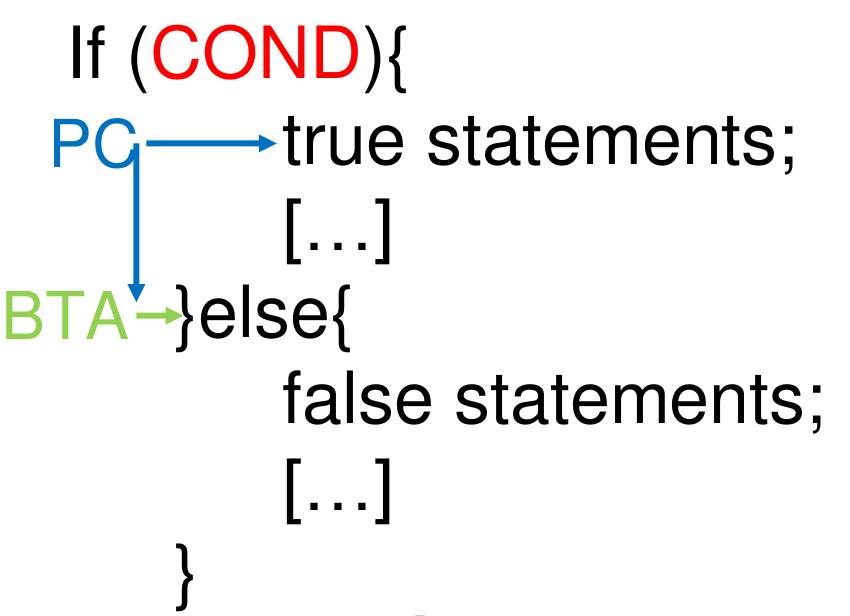
\includegraphics[scale=0.22]{Branch_Target_Buffer.png}
  %  \caption{Branch target buffer}
  %  \label{fig:Branch target buffer}
  %\end{figure}
\end{tabular}

\subsubsection{Execution of conditional branches for 5-stage MIPS pipeline}

\[ beq\ \$x,\$y,\ \text{offset} \]

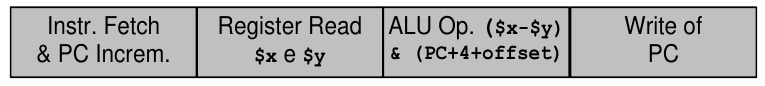
\includegraphics[scale=0.6]{Execution_of_conditional_branches_for_5-stage_MIPS_pipeline.png}

\begin{enumerate}
  \item Instruction fetch and PC increment
  \item Registers read (\$x and \$y) from Register File.
  \item ALU operation to compare registers (\$x and \$y) to derive
  Branch Outcome (branch taken or branch not taken). Computation of Branch Target Address (PC+4+offset):
  the value (PC+4) is added to the least significant 16
  bit of the instruction after sign extension
  \item The result of registers comparison from ALU is used to
  decide the value to be stored in the PC: (PC+4) or
  (PC+4+offset).    
\end{enumerate}

Results:
\begin{itemize}
  \item Branch Outcome and Branch Target Address are
  ready at the end of the EX stage (3th stage)
  \item Conditional branches are solved when PC is updated
  at the end of the ME stage (4th stage)
\end{itemize}

\textbf{The Problem of Control Hazards}

Control hazards: Attempt to make a decision on the next instruction to fetch before the branch
condition is evaluated.

\paragraph{Branch Hazards: Example}

\begin{figure}[h!]
  \centering
  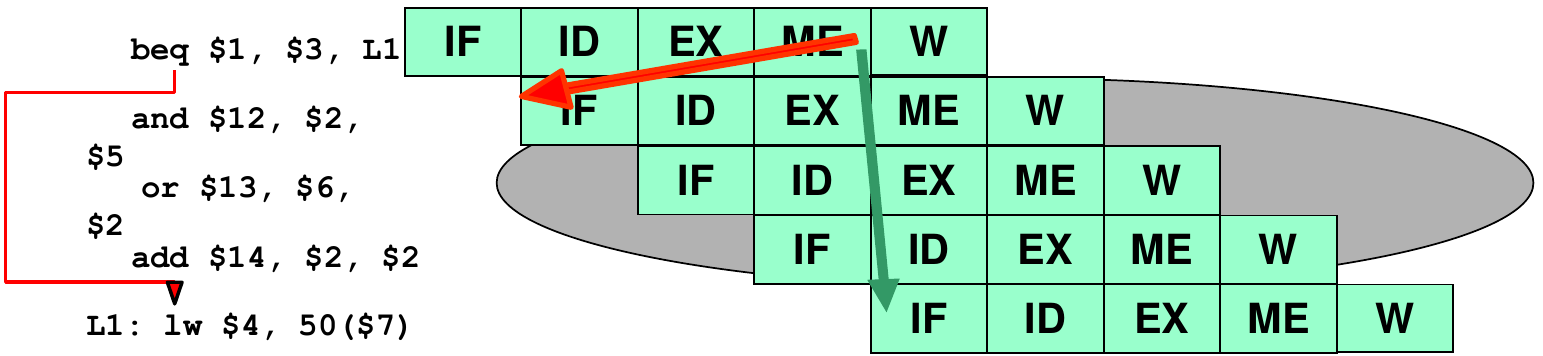
\includegraphics[scale=0.3]{Branch_Hazards_Example.png}
\end{figure}

The branch instruction may or may not change the PC in MEM stage, but the next 3 instructions are fetched and their execution is
started.
\begin{itemize}
  \item If the \textbf{branch} is \textbf{not taken}, the pipeline \textbf{execution} is \textbf{OK}
  \item If the \textbf{branch} is \textbf{taken}, it is necessary to \textbf{flush} the \textbf{next 3 instructions}
  in the pipeline and fetched the lw instruction at the branch target
  address (L1) 
\end{itemize}

\newpage

\subsubsection{Branch Stalls without/with Forwarding}

\begin{tabular}{m{24em} m{24em}}
  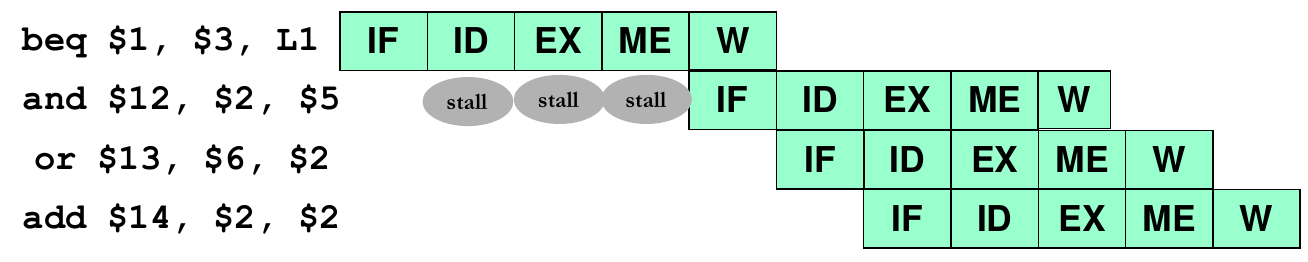
\includegraphics[scale=0.23]{Branch_Stalls_without_Forwarding.png}
  &
  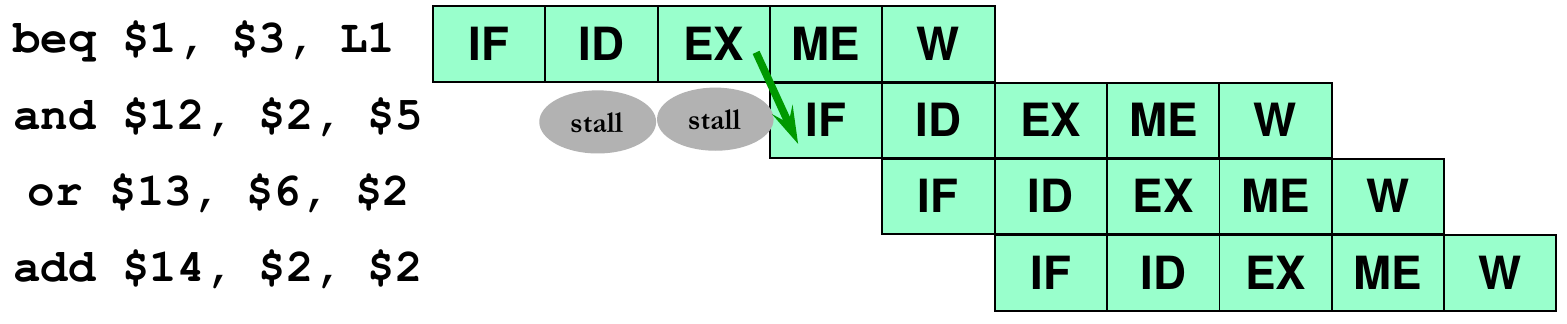
\includegraphics[scale=0.2]{Branch_Stalls_with_Forwarding.png}
  \\
  Without forwarding
  & 
  With forwarding
\end{tabular}

To stall the pipeline until the branch decision is taken (stalling until resolution) and then fetch the
correct instruction flow:
\begin{itemize}
  \item \textbf{Without forwarding:} three clock cycles
  \item \textbf{With forwarding:} for two clock cycles  
\end{itemize}

If the branch is not taken, the three cycles penalty is not justified $\rightarrow$ throughput reduction.

\smallskip

We can assume the branch not taken, and flush the next 3 instructions in the pipeline only if the
branch will be taken.

\paragraph{Early Evaluation of the PC}
To improve performance in case of branch hazards, \textbf{we need to add hardware resources} to:
\begin{enumerate}
  \item Compare registers to derive branch outcome
  \item Compute branch target address
  \item Update the PC register  
\end{enumerate}
as soon as possible in the pipeline.

\smallskip

\begin{remarks}
  MIPS processor compares registers, computes branch target address and updates PC during ID stage.  
\end{remarks}

\begin{figure}[ht!]
  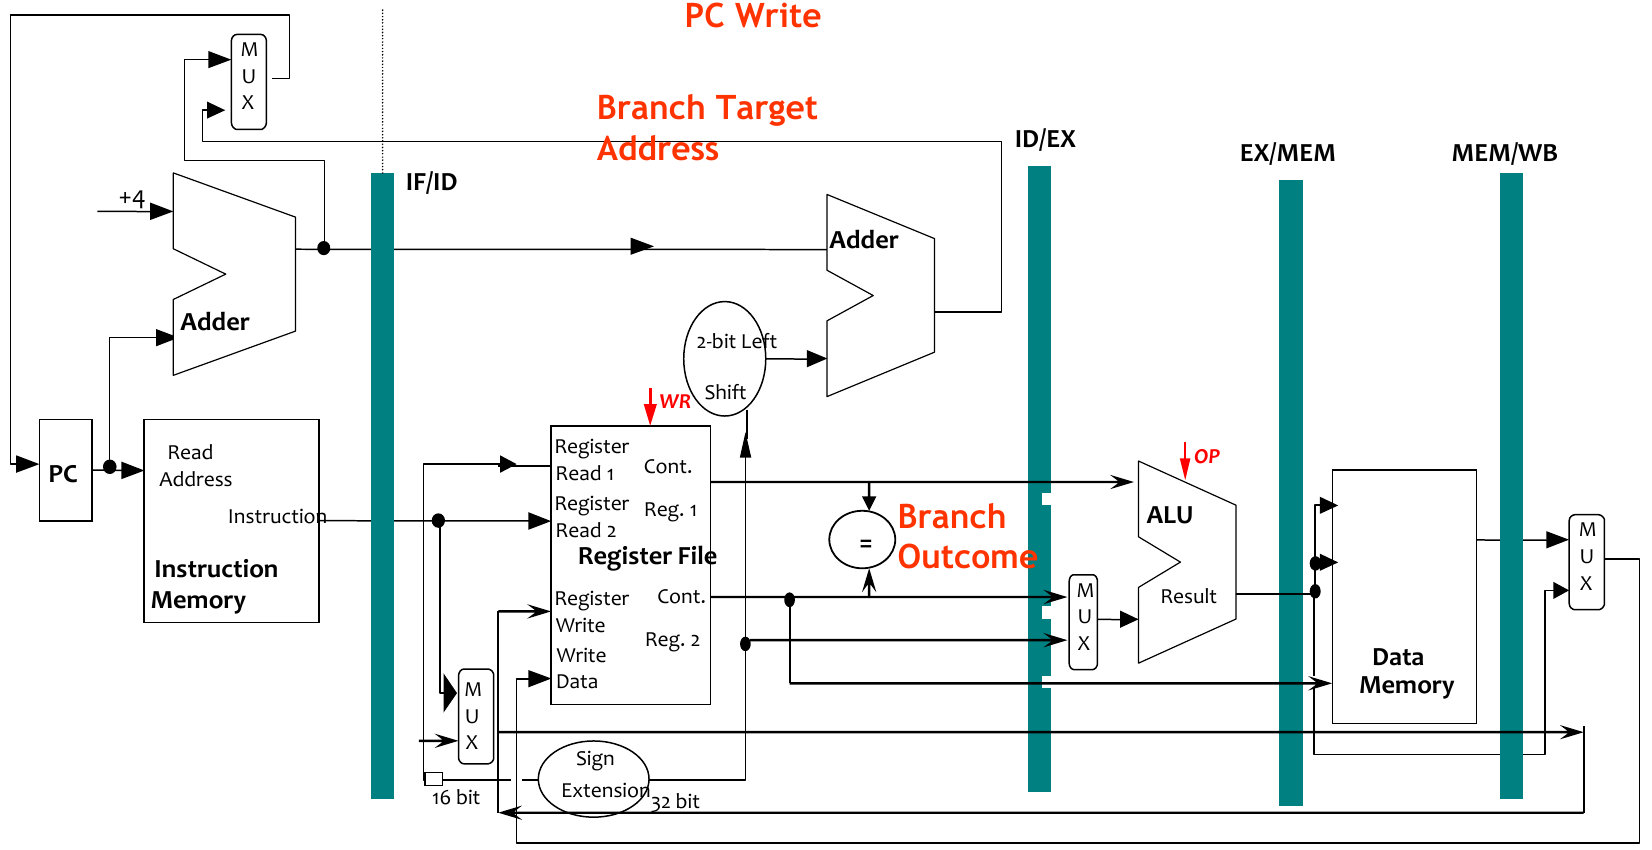
\includegraphics[scale=0.38]{MIPS_Processor_Early_Evaluation_of_the_PC.png}
\end{figure}

\newpage

The final result is:
\begin{figure}[ht!]
  \centering
  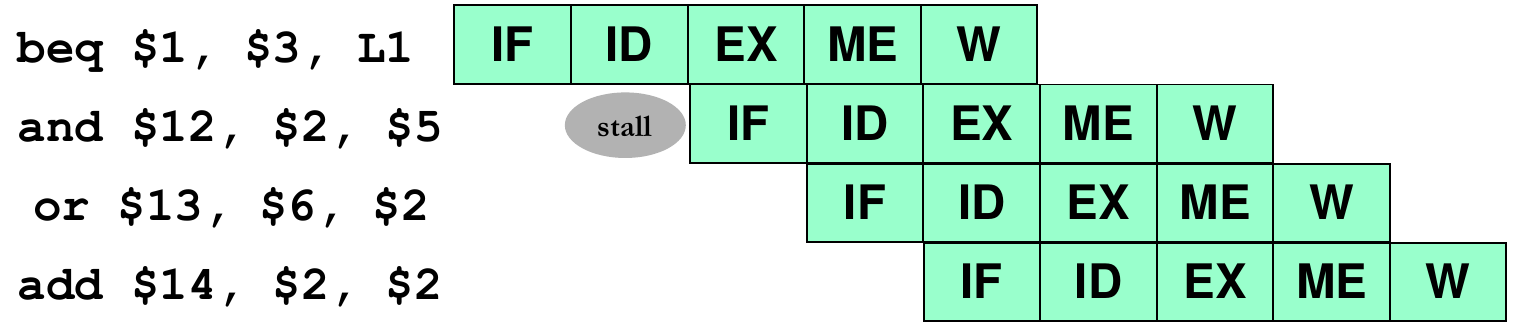
\includegraphics[scale=0.3]{Images/MIPS_Processor_Early_Evaluation_of_the_PC_2.png}
\end{figure}


\textbf{Issue:} But there is another problem in some situation (es. loops):

\begin{figure}[ht!]
  \centering
  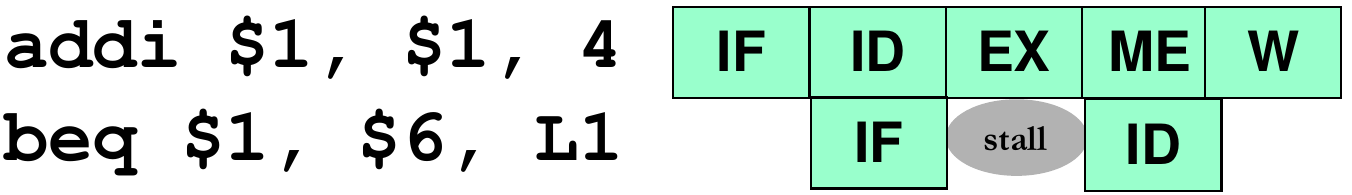
\includegraphics[scale=0.3]{Early_Evaluation_of_the_PC_an_issue.png}
\end{figure}

In that case we have a Data Dependece on \$1, since the computation of \$1 is 
ready after the execution stage of addi, to compute the evaluation of beq 
we have to wait until the value is ready (otherwise we wuold use the old value 
of \$1).

We know that after a branch instruction we have 1 stall, so in the instruction
after beq we have to put another stall.

\medskip

With the branch decision made during ID stage, there is
a reduction of the cost associated with each branch
\begin{remarks} \textbf{Branch penalty:}
  We need
  \begin{itemize}
    \item only one-clock-cycle stall after each branch
  \end{itemize}
  Or
  \begin{itemize}
    \item a flush of only one instruction following the branch 
  \end{itemize}
  This is related to branch itself, not considering problems related data dependences.
\end{remarks}

\subsection{Introduction to branch prediction}

The main goal of the \textbf{branch prediction} is to evaluate as early as possible the outcome of a branch instruction.
Its performance depends on:

\begin{itemize}
  \item The \textbf{accuracy}, measured in terms of the percentage of incorrect predictions given
  \item The \textbf{cost of an incorrect prediction} measured in terms of time lost to execute useless instructions \textit{(misprediction penalty)} given by the processor architecture
        \begin{itemize}
          \item the cost increases for deeply pipelined processors
        \end{itemize}
  \item \textbf{Branch frequency} given by the application
        \begin{itemize}
          \item the importance of accurate branch prediction is higher in programs with higher branch frequency
        \end{itemize}
\end{itemize}

\smallskip

There are many methods to deal with performance loss due to branch hazards:

\begin{itemize}
  \item \textbf{Static} branch prediction techniques: the actions for a branch are fixed for each branch during the entire execution
        \begin{itemize}
          \item used in processors where the expectation is that the branch behaviour is highly predictable at compile time
          \item can be used to assist dynamic predictors
        \end{itemize}
  \item \textbf{Dynamic} branch prediction techniques: the actions for a branch can change during the program execution
\end{itemize}

In both cases, care must be taken not to change the processor state until the branch is definitely known.

\newpage

\subsection{Static techniques}

There are \(5\) commonly used branch prediction techniques:

\begin{itemize}
  \item Branch \textbf{always not taken}
  \item Branch \textbf{always taken}
  \item Backward \textbf{taken forward not taken}
  \item Profile \textbf{driven prediction}
  \item Delayed \textbf{branch}
\end{itemize}

Each one of these techniques will be discussed in the following Sections \textit{(from \ref{sec:branch-always-not-taken} to \ref{sec:delayed-branch})}.

\subsubsection{Branch Always Not Taken}
\label{sec:branch-always-not-taken}

The branch is always assumed as \textbf{not taken}, thus the sequential instruction flow that has been fetched can continue as if the branch condition was not satisfied.
\begin{itemize}
  \item If the condition in stage \texttt{ID} will result in not satisfied \textit{(and the prediction is correct)} performance can be preserved.
  \item If the condition in stage \texttt{ID} will result in satisfied \textit{(and the prediction is incorrect)} the branch is taken: the next instruction already fetched is flushed \textit{(turned into a \texttt{nop})} and the execution is restarted by fetching the instruction at the branch target address.
  There is a one-cycle penalty. 
\end{itemize}

\begin{figure}[htbp]
  \bigskip
  \centering
  \tikzfig[1]{image-11.tikz}
  \caption{Branch always not taken: success}
  \label{fig:branch-always-not-taken}
  \bigskip
\end{figure}

\begin{figure}[htbp]
  \bigskip
  \centering
  \tikzfig[1]{image-12.tikz}
  \caption{Branch always not taken: fail}
  \label{fig:branch-always-not-taken-fail}
  \bigskip
\end{figure}



\subsubsection{Branch Always Taken}
\label{sec:branch-always-taken}

An alternative scheme is to consider \textbf{every branch as taken}: as soon as the branch is decoded and the branch target address is computed, the branch is assumed to be taken and the fetching and the execution stages can begin at the target.

The predicted-taken scheme makes sense for pipelines where the branch target is known before the actual outcome.
This is not the case within \textit{MIPS} pipeline \textit{(where the branch target is known only after the operation outcome)}, so \textbf{there is no advantage in this approach}.

\newpage

\subsubsection{Backward Taken Forward Not Taken}
\label{sec:backward-taken-forward-not-taken}

The prediction is based on the branch direction:

\begin{itemize}
  \item \textbf{Backward} going branches are predicted as \textbf{taken}
        \begin{itemize}
          \item the branches at the end of loops are likely to be executed most of the time
        \end{itemize}
  \item \textbf{Forward} going branches are predicted as \textbf{not taken}
        \begin{itemize}
          \item the \textbf{if} branches are likely not executed most of the time
        \end{itemize}
\end{itemize}

\subsubsection{Profile Driven Prediction}
\label{sec:profile-driven-prediction}

The branch prediction is \textit{based} on profiling information collected \textit{from earlier runs}.
This method can use compiler hints, and it's potentially more effective than the other ones;
however, it's also the most complicated between the \(5\) as it needs additional hardware.

This technique will be explored in Section~\ref{sec:dynamic-branch-prediction}.

\subsubsection{Delayed Branch}
\label{sec:delayed-branch}

The compiler statically schedules an independent instruction in the branch delay slot, which is then executed whether or not the branch is taken.

If the branch delay consists of one cycle (as in \textit{MIPS}), there's only one delay slot;
almost all processors with delayed branches have a single delay slot, as it's difficult for the compiler to fill more than one of them.

If the branch:

\begin{itemize}
  \item \textbf{Is untaken}: the execution continues with the instruction after the branch
  \item \textbf{Is taken}: the execution continues at the branch target
\end{itemize}

\begin{figure}[htbp]
  \bigskip
  \centering
  \tikzfig[1]{image-13.tikz}
  \caption{Delayed branch}
  \label{fig:delayed-branch}
  \bigskip
\end{figure}

The compiler's job is to make the instruction placed in the branch delay slot valid and useful.
There are three ways in which the branch delay slot can be scheduled:

\begin{enumerate}
  \item From \textbf{before}
  \item From \textbf{target}
  \item From \textbf{fall through}
\end{enumerate}

These methods will be better analyzed in the following paragraphs.

\bigskip
In general, the compilers can fill about \textbf{half} of the delayed branch slots with valid and useful instructions, while the remaining slots are filled with \texttt{nop}.
In deeply pipelined processors, the delayed branch is longer than one cycle: many slots must be filled for every branch, thus it's more difficult to fill each of them with \textit{useful} instructions.

\bigskip
The main limitations on delayed branch scheduling arise from:

\begin{itemize}
  \item \textbf{The restriction on the instruction} that can be scheduled in the delay slot
  \item \textbf{The ability of the compiler} to statically predict the outcome of the branch
\end{itemize}

To improve the ability of the compiler to fill the branch delay slot, most processors have introduced a \textbf{cancelling or nullifying branch}.
The instruction includes the direction of the predicted branch:

\begin{itemize}
  \item When the branch \textbf{behaves as predicted}, the instruction in the branch delay slot is \textbf{executed normally}
  \item When the branch \textbf{is incorrectly predicted}, the instruction in the branch delay slot is \textbf{flushed} \textit{(turned into a \texttt{nop})}
\end{itemize}

With this approach, the compiler does not need to be as conservative when filling the delay slot.

\paragraph{From before}

The branch delay slot is scheduled with an independent instruction \textbf{from before the branch}.

The instruction in the branch delay slot is always executed, whether the branch is taken or not.
An illustration of this strategy is represented in Figure~\ref{fig:from-before}.

\begin{figure}[htbp]
  \bigskip
  \centering
  \tikzfig[1]{image-14.tikz}
  \caption{From before}
  \label{fig:from-before}
  \bigskip
\end{figure}

\begin{remarks}
  When to use it: when there exists a indipendent instruction before the branch 
\end{remarks}

\paragraph{From target}

The use of a register in the branch condition prevents any instructions with that 
register as a destination from being moved after the branch itself (\$1 in our case).

\smallskip

The branch delay slot is scheduled from \textbf{the target of the branch} \textit{(usually the target instruction will need to be copied because it can be reached by another path)}.

\smallskip

This strategy is preferred when the branch is taken with high probability, such as loop branches \textbf{(backward branches)}.
An illustration of this strategy is represented in Figure~\ref{fig:from-target}.

\begin{figure}[htbp]
  \bigskip
  \centering
  \tikzfig[1]{image-15.tikz}
  \caption{From target}
  \label{fig:from-target}
  \bigskip
\end{figure}

In other word: if there is high probability that i take the branch, i can put an instruction 
of the target branch since i will (high) probably execute it. I have to rewrite the target 
instruction because it can be reached by another path.

\begin{remarks}
  When to use it: when there is an high probability that the branch is taken (loops) 
\end{remarks}

\paragraph{From fall through}

The use of a register in the branch condition prevents any instructions with that register as a destination from being moved after the branch itself \textit{(like what happens in the from target technique)}.
The branch delay slot is scheduled with an instruction from \textbf{the not taken fall through path}.

This strategy is \textit{preferred} when the branch \textit{is not taken with high probability}, such as \textbf{forward branches}.

\begin{figure}[htbp]
  \bigskip
  \centering
  \tikzfig[1]{image-16.tikz}
  \caption{From fall through}
  \label{fig:from-fall-through}
  \bigskip
\end{figure}

NON HO CAPITO QUESTA PARTE: 

\smallskip

In order to make the optimization legal for the target, 
it must be ok to execute the moved instruction when the branch goes in the unexpected direction;
the instruction in the branch delay slot is executed but its result is wasted 
\textit{(if the program will still execute correctly)}.

For example, if the destination register is an unused temporary register when the branch goes in an unexpected direction.

\begin{remarks}
  When to use it: when there is an high probability that the branch is not taken (if) 
\end{remarks}

\newpage

\subsection{Dynamic Branch Prediction}
\label{sec:dynamic-branch-prediction}

\begin{remarks}
  Questa parte il prof dice sarà quasi sicuramente esercizi 
\end{remarks}

\textit{Basic idea}: use the past branch behaviour to predict the future.

The prediction will depend on the behavior of the branch at \textbf{run time} and
will change if the branch changes its behavior \textbf{during execution}.

\medskip
What do we have to predict/compute? 
\begin{enumerate}
  \item \textbf{Branch Outcome Predictor} \textit{(BOP)} (Do I or not take the jump?)
        \begin{itemize}
          \item used to predict the direction of a branch \textit{(taken or not taken)} 
        \end{itemize}
  \item \textbf{Branch Target Predictor} \textit{(BTP)} (Which is the address of the next instruction?)
        \begin{itemize}
          \item used to predict the branch target address in case of taken branch
        \end{itemize}
\end{enumerate}

\medskip

These modules are used by the \textit{Instruction Fetch Unit} to predict the next instruction to read in the instruction cache \textit{(also called I-cache)}:

\begin{itemize}
  \item Branch \textbf{is not taken}: \texttt{PC} is incremented
  \item Branch \textbf{is taken}: \textit{BTP} gives the target address
\end{itemize}

How to do all of that? Branch target buffer.

\subsubsection{Branch Target Buffer}

The \textbf{Branch Target Buffer} is a cache storing the predicted branch target address for the next instruction after a branch.
The \textit{BTB} is accessed in the \texttt{IF} stage using the instruction address of the fetched instruction \textit{(a possible branch)} to index the cache.

The typical entry of the \textit{BTB} is shown in Figure~\ref{fig:typical-entry-BTB}.
The predicted target address is expressed as \texttt{PC}-relative.

\begin{figure}[htbp]
  \smallskip
  \centering
  \tikzfig[1]{image-17.tikz}
  \caption{Typical entry of the \textit{BTB}}
  \label{fig:typical-entry-BTB}
  \smallskip
\end{figure}

The structure and operation of the \textit{BTB} is shown in Figure~\ref{fig:structure-of-BTB}.

\begin{figure}[htbp]
  \smallskip
  \centering
  \tikzfig[0.8]{image-18.tikz}
  \caption{Structure of the \textit{BTB}}
  \label{fig:structure-of-BTB}
  \smallskip
\end{figure}

\begin{remarks}
  MA CHE POI: come funziona se io trovo il PC nel BTB ma essendo solo i k meno significativi
  io potrei anche aver memorizzato anche un istruzione sbagliata.
  Nel caso poi la previsione sia taken quando mi accorgo che i due BTA (quello memorizzato
  nella BTB e quello invece vero) sono diversi?  

  MI sa che noi in realtà calcoliamo sempre se il salto va preso (ovviamente) ma anche il BTA,
  quello che stiamo facendo è solo predizione!
\end{remarks}


\subsubsection{Branch History Table}

The \textbf{Branch History Table} contains \(1 \, bit\) for each entry that says whether the branch was recently taken or not.
It is indexed by the lower portion of the address of the branch instruction.
The structure of the \textit{BTB} is shown in Figure~\ref{fig:structure-of-BHT}.

\begin{figure}[htbp]
  \bigskip
  \centering
  \tikzfig[1]{image-19.tikz}
  \caption{Structure of the \textit{BHT}}
  \label{fig:structure-of-BHT}
  \bigskip
\end{figure}

\begin{remarks}
  For each PC, the BTB stores:
  \begin{itemize}
    \item if the PC is a branch
    \item if the branch is predicted taken/not taken (BHT - BOP)
    \item the address of the branch if taken (BTP)
  \end{itemize}
\end{remarks}

The prediction is a hint that it is assumed to be correct and fetching begins in the predicted direction.
If the hint turns out to be wrong, the prediction bit is inverted and stored back;
the pipeline is then flushed and the correct sequence is executed.

The table has no tags \textit{(every access is a hit)} and the prediction bit could have been put there by another branch with the same LSBs.
The \(1\)-bit branch history table only considers the last status of the branch \textit{(either taken or not taken)}.
It is a simple \textit{FSA} where a misprediction will change the current value, whose structure is shown in Figure~\ref{fig:BHT-as-FSA}.

\begin{figure}[htbp]
  \bigskip
  \centering

  \begin{tikzpicture}[auto, node distance=3cm, >=Triangle]
    \node [state, minimum size=1.5cm](0) {\texttt{NT}};
    \node [state, right= of 0, minimum size=1.5cm](1) {\texttt{T}};

    \path[->, thick]
    (0) edge [loop left] node {\texttt{NT}} ()
    (1) edge [loop right] node {\texttt{T}} ()
    (0) edge [bend left] node {\texttt{T}} (1)
    (1) edge [bend left] node {\texttt{NT}} (0);

  \end{tikzpicture}

  \caption{\(1\)-bit \textit{BHT} as \textit{FSA}}
  \label{fig:BHT-as-FSA}
  \bigskip
\end{figure}

A \textbf{misprediction} occurs when:

\begin{itemize}
  \item The prediction is \textbf{incorrect} for that branch
  \item The same index has been referenced by two different branches, and the \textbf{the previous history refers to the other branch}
        \begin{itemize}
          \item to solve this problem it's enough to increase the number of rows in the \textit{BHT} or to use a hashing function \textit{(such as  GShare)}.
        \end{itemize}
\end{itemize}

\bigskip
In a loop branch, even if a branch is almost always taken and then not taken one, the \(1\)-bit \textit{BHT} will mispredict \textbf{twice} \textit{(rather than once)} when it is not taken.
That situation causes two wrong predictions:
\begin{itemize}
  \item At the \textbf{last loop iteration}
        \begin{itemize}
          \item the loop must be exited
          \item the prediction bit will say \texttt{TAKE}
        \end{itemize}
  \item While \textbf{re-entering the loop}
        \begin{itemize}
          \item at the end of the first iteration the branch must be taken to stay in the loop
          \item the prediction bit will say \texttt{NOT TAKE} because the bit was flipped on the previous execution of the last iteration of the loop
        \end{itemize}
\end{itemize}

\smallskip

To fix this kind of behaviour, the \(2\)-bit \textit{BHT} was introduced.

\subsubsection{\textit{2}-bit Branch History Table}

By adding one bit to the \textit{BHT}, the prediction must miss twice before it is changed.
In a loop branch, there's no need to change the prediction for the last iteration.

For each index in the table, the \(2\) bits are used to encode the four states of a \textit{FSA}.
Its structure is represented in Figure~\ref{fig:2-bit-BHT-as-FSA}.

\begin{figure}[htbp]
  \bigskip
  \centering

  \scalebox{0.7}{
    \begin{tikzpicture}[auto, node distance=3cm, >=Triangle]
      \node [state, minimum size=2cm](nt_strong) {\texttt{NT strong}};
      \node [state, below= of nt_strong, minimum size=2cm](t_weak) {\texttt{T weak}};
      \node [state, right= of nt_strong, minimum size=2cm](nt_weak) {\texttt{NT weak}};
      \node [state, below= of nt_weak, minimum size=2cm](t_strong) {\texttt{T strong}};

      \path[->, thick]
      (nt_strong) edge [loop left] node {\texttt{NT}} ()
      (t_strong) edge [loop right] node {\texttt{T}} ()
      (nt_strong) edge [bend left] node {\texttt{T}} (nt_weak)
      (nt_weak) edge [bend left] node {\texttt{NT}} (nt_strong)
      (t_weak) edge [bend left] node {\texttt{T}} (t_strong)
      (t_strong) edge [bend left] node {\texttt{NT}} (t_weak)
      (t_weak) edge [bend left] node {\texttt{NT}} (nt_strong)
      (nt_weak) edge [bend left] node {\texttt{T}} (t_strong);
    \end{tikzpicture}
  }

  \caption{\(2\)-bit \textit{BHT} as \textit{FSA} (FSA = four state algorithm (?))}
  \label{fig:2-bit-BHT-as-FSA}
  \bigskip
\end{figure}

\subsubsection{\textit{k}-bit Branch History Table}

It's a generalization: \(n\)-bit saturating counter for each entry in the prediction buffer.

The counter can take on values between \(0\) and \(2^{n-1}\).
When the counter is greater than or equal to one-half of its maximum value, the branch is predicted as taken.
Otherwise, it's predicted as untaken.

As in the \(2\)-bit scheme, the counter is incremented on a taken branch and decremented on an untaken branch.
Studies on \(n\)-bit predictors have shown that \(2\) bits behave almost as well \textit{(so using more than \(2\) bits is almost useless)}.

\newpage

\subsection{Correlating Branch Predictors}

\begin{remarks}
  Questa parte il prof dice sarà sopratutto nella teoria
\end{remarks}

\textit{Basic idea}: the behaviour of recent branches is correlated, that is the recent behaviour of other branches rather than just the current branch that we are trying to predict can influence the prediction of the current branch.

\medskip

The \textbf{Correlating Branch Predictors} are predictors that use the behaviour of other branches to make a prediction.
They are also called \textit{\(2\)-level Predictors}.
Their scheme is represented in Figure~\ref{fig:structure-of-CBP}.

A \((1, 1)\) Correlating Predictor denotes a \(1\)-bit predictor with \(1\)-bit of correlation: the behaviour of the last branch is used to choose among a pair of \(1\)-bit branch predictors.

\begin{figure}[htbp]
  \smallskip
  \centering
  \tikzfig[0.8]{image-20.tikz}
  \caption{Structure of the \textit{Correlating Branch Predictors}}
  \label{fig:structure-of-CBP}
  \smallskip
\end{figure}

\begin{remarks}
  La mia predizione in questo caso sarà funzione del risultato (non la predizione!) del'ultimo branch:
  \begin{itemize}
    \item Se l'ultimo branch prima di quello che sto valutando è stato \textbf{not taken}:
    \begin{itemize}
      \item Prenderò in cosiderazione la BHT T0
    \end{itemize}
    \item Se l'ultimo branch prima di quello che sto valutando è stato \textbf{taken}:
    \begin{itemize}
      \item Prenderò in cosiderazione la BHT T1
    \end{itemize}
  \end{itemize}
\end{remarks}

\newpage

\subsubsection{\textit{(m, n)} Correlating Branch Predictors}

In general, \((m, n)\) correlating predictors records last \(m\) branches to choose from \(2^m\) \textit{BHTs}, each of which is a \(n\)-bit predictor.

The branch prediction buffer can be indexed by using a concatenation of low order bits from the branch address with \(m\)-bit global history \textit{(i.e. global history of the most recent \(m\) branches, implemented with a shift register)}.

The general structure of a \((m, n)\) \textit{CBP} is represented in Figure~\ref{fig:m-n-CBP}.

\begin{figure}[htbp]
  \smallskip
  \centering
  \tikzfig[0.8]{image-21.tikz}
  \caption{Structure of the \textit{(m, n) Correlating Branch Predictors}}
  \label{fig:m-n-CBP}
  \smallskip
\end{figure}

\paragraph{A \textit{(2, 2) Correlating Branch Predictor}}

A \((2, 2)\) correlating predictor has \(4\) \(2\)-bit Branch History Tables.
It uses the \(2\)-bit global history to choose among the \(4\) \textit{BHTs}.

\begin{itemize}
  \item Each \textit{BHT} is composed of \(16\) entries of \(2\)-bit each
  \item The \(4\)-bit branch address is used to choose four entries \textit{(a row)}
  \item \(2\)-bit global history is used to choose one of four entries in a row \textit{(one of the four \textit{BHTs})}
\end{itemize}

\begin{figure}[htbp]
  \smallskip
  \centering
  \tikzfig[0.8]{image-21-copy.tikz}
  \caption{Structure of the \textit{(2, 2) Correlating Branch Predictors}}
  \label{fig:2-2-CBP}
  \smallskip
\end{figure}

\paragraph{Accuracy of Correlating Predictors}

A \(2\)-bit predictor with no global history is simply a \((0, 2)\) predictor.

By comparing the performance of a \(2\)-bit simple predictor with \(4000\) entries and a \(2, 2\) correlating predictor with \(1000\) entries, we find out that the latter not only outperforms the \(2\)-bit predictor with the same number of total bits but also often outperforms a \(2\)-bit predictor with an unlimited number of entries.

\newpage

\subsection{Two Level Adaptive Branch Predictors}

\begin{remarks}
  Questa parte da non fare: il prof non la spiega, serve solo per farci capire che
  si può sempre fare meglio, ma deve valerne la pena
\end{remarks}

The first level history is recorded in one \textit{(or more)} \(k\)-bit shift register called \textit{Branch History Register (BHR)} which records the outcomes of the \(k\) most recent branches.
The second level history is recorded in one \textit{(or more)} tables called \textit{Pattern History Table (PHT)} of two bits saturating counters.

The BHR is used to index the PHT to select which \(2\)-bit counter to use.
Once the two-bit counter is selected, the prediction is made using the same method as in the two bits counter scheme.

\subsubsection{GA and GShare Predictors}

The \textbf{GA Predictor} \textit{(Genetic Algorithm Predictor)} is composed of a \textit{BHT} \textit{(local predictor)} and by one or more \textit{GAs} \textit{(local and global predictor)}:

\begin{itemize}
  \item The \textit{BHT} is indexed by the low order bits of the \texttt{PC} \textit{(the branch address)}
  \item The \textit{GAs} are a \(2\)-level predictor: \textit{PHT} is indexed by the content of \textit{BHR} \textit{(from global history)}
\end{itemize}

\bigskip

The \textbf{GShare Predictor} is a local \texttt{XOR} global information, indexed by the exclusive \texttt{OR} of the low order bits of \textit{PC} \textit{(branch address)} and the content of \textit{BHR} \textit{(global history)}.

\bigskip
The structure of a \textit{GA} predictor is represented in Figure~\ref{fig:GA-predictor}, while Figure~\ref{fig:GShare-predictor} shows the structure of a \textit{GShare} predictor.

\begin{figure}[htbp]
  \bigskip
  \centering
  \begin{minipage}[b]{0.6\textwidth}
    \centering
    \tikzfig[0.6]{image-22.tikz}
    \caption{GA Predictor}
    \label{fig:GA-predictor}
  \end{minipage}
  \begin{minipage}[b]{0.39\textwidth}
    \centering
    \tikzfig[0.6]{image-23.tikz} % 6pt too wide with 0.6 zoom
    \caption{GShare Predictor}
    \label{fig:GShare-predictor}
  \end{minipage}
  \bigskip
\end{figure}

\clearpage

\section{Instruction Level Parallelism - \textit{ILP}}

\begin{remarks} ILP: \hfill % \break 
  \begin{itemize}
    \item Whats is? Architectural technique that allows the overlap of individual machine operations ( add, mul, load, store ...)
    \item What consist in? Multiple operations will execute in parallel (simultaneously)
    \item Goal: Speed Up the execution
  \end{itemize}
\end{remarks}

The objective of the \textit{ILP} is to improve the \textit{CPI}, with the ideal goal of \(1\) \textit{cycle per instruction}.

\begin{definition}
  The \textit{ILP} = potential overlap of execution among unrelated instructions   
\end{definition}

This goal is only achievable if there is no \textbf{hazards} \textit{(as described in Section~\ref{sec:pipeline-hazards})}.

\medskip
Two properties are critical to program correctness \textit{(and normally preserved by maintaining both data and control dependences)}:

\begin{enumerate}
  \item \textbf{Exception behaviour}: preserving exception behaviour means that any changes in the ordering of instructions execution must not change how exceptions are raised in the program
  \item \textbf{Data flow}: the actual flow of data values among instructions that produce the correct results and consume them
\end{enumerate}

\paragraph{ILP vs Parallel Processing}

\begin{tabular}{m{24em} m{24em}}
  ILP (even single core) & PARALLEL PROCESSING
  \\
  \begin{itemize}
    \item  Overlap individual machine operations (add, mul, load...) so that they execute in parallel
    \item Transparent to the user
    \item Goal: speed up execution
  \end{itemize}
  & 
  \begin{itemize}
    \item Having separate processors getting separate chunks of the program (processors programmed to do so)
    \item Nontransparent to the user
    \item Goal: speed up and quality up
  \end{itemize}
\end{tabular}

\subsection{Strategies to support \textit{ILP}}
\label{sec:strategies-to-support-ilp}

There are main two software strategies to support \textit{ILP}:

\begin{enumerate}
  \item \textbf{Dynamic} scheduling: depends on the hardware to locate parallelism
  \item \textbf{Static} scheduling: relies on the software to identify potential parallelism
\end{enumerate}

Usually, hardware-intensive approaches dominate desktop and server markets.

\subsubsection{Dynamic scheduling}

The hardware reorders the instruction execution to reduce pipeline stall while maintaining data flow and exception behaviour.

\medskip
\textit{Properties of the Dynamic Scheduling}:

\begin{enumerate}
  \item Instructions are fetched and \textbf{issued in program order}
  \item Execution begins \textbf{as soon as operands are available}, possibly out of order execution
  \item Out of order execution introduces possibility or \textit{WAR} and \textit{WAW} data hazards
  \item Out of order execution implies \textbf{out of order completion}
        \begin{itemize}
          \item a \textit{reorder buffer} is needed to reorder the output
        \end{itemize}
\end{enumerate}

\smallskip
The two main techniques used by hardware to minimize stalls are:

\begin{itemize}
  \item \textbf{Forwarding}
        \begin{itemize}
          \item The result from the \texttt{EX/MEM} and the \texttt{EX/WB} pipeline registers is \textbf{fed back} (rimmessi) to the \texttt{ALU} inputs
          \item If the forwarding hardware detects that the previous \texttt{ALU} operation has \textbf{written the register corresponding to a source for the current} \texttt{ALU} operation:
                \begin{itemize}
                  \item control logic selects the forwarded result as the \texttt{ALU} input
                  \item the value read from the register file is discarded
                \end{itemize}
          \item The \texttt{ALU} needs \textbf{multiplexers} that allow it to select the correct inputs from the pipeline
          \item This technique can be generalized to include \textbf{passing a result directly to the functional unit} that requires it
                \begin{itemize}
                  \item in that case, a result is forwarded from the pipeline register corresponding to the output of one unit to the input of another, rather than just from the result of a unit to the input of the same unit
                \end{itemize}
        \end{itemize}
  \item \textbf{Stalling}
        \begin{itemize}
          \item Since not all potential data hazards can be solved by bypassing, a piece of hardware called \textit{pipeline interlock} is added
          \item When it detects a hazard, it \textbf{stalls} the pipeline until that hazard it solved
          \item The stalls are often referred to as \inlinequote{bubbles}
        \end{itemize}
\end{itemize}

\medskip
\textbf{Advantages} of dynamic scheduling:
\begin{itemize}
  \item It enables handling some cases where dependencies are \textbf{unknown} at compile time
  \item It \textbf{simplifies} the compiler complexity
  \item It allows compiled code to run \textbf{efficiently} on a different pipeline
\end{itemize}

\textbf{Disadvantages}:
\begin{itemize}
  \item A significant increase in \textbf{hardware complexity}
  \item Increased \textbf{power consumption}
  \item Could generate \textbf{imprecise exception}
\end{itemize}

\newpage

\subsubsection{Scoreboard CDC6600}
\label{par:CDC6600-scoreboard}

As discussed earlier \textit{(Section~\ref{sec:instructions-issuing})}, a specific data structure is needed to solve data dependences without specialized compilers.
The first implementation of such hardware is found in the \textbf{CDC6600 Scoreboard}, \textit{(1963)}.

\begin{remarks} \hfill
  \begin{itemize}
    \item \textbf{Starting Situation:} a 6-stages complex pipeline with floating point operation and issue-phase.  
    \item \textbf{Problem:} data dependences that cannot be hidden with bypassing or forwarding cause hardware stalls of the pipeline
    \item \textbf{Solution:} allow instructions behind a stall to proceed: HW rearranges the instruction execution to reduce stalls
    \begin{itemize}
      \item Enables out-of-order execution and completion (commit): Out-of order execution introduces possibility of WAR, WAW data hazards
    \end{itemize}
  \end{itemize}
\end{remarks}



\begin{remarks} \textbf{When is it Safe to Issue an Instruction?} \hfill \break
  Suppose a data structure keeps track of all the instructions in all the functional units
  The following checks need to be made before the Issue stage can dispatch (spedire) an instruction
  \begin{itemize}
    \item Is the required function unit available?
    \item Is the input data available? → RAW?
    \item Is it safe to write the destination? → WAR? WAW?
    \item Is there a structural conflict at the WB stage?
  \end{itemize}
\end{remarks}



With the result of a \(250\%\) speedup with regards to no dynamic scheduling and a \(170\%\) speedup with regards to instructions reordering by the compiler.
It has the downside of having a \textbf{slow memory} \textit{(due to the absence of cache)} and \textbf{no forwarding hardware}.
Furthermore, it has a low number of \textit{FUs} and it does not issue structural hazards.

It solves the issue of data dependencies that cannot be hidden with bypassing or forwarding due to the hardware stalls of the pipeline by allowing out-of-order execution and commit of instructions.

\medskip

textbf{The scoreboard centralizes hazard management}:
\begin{enumerate}
  \item \textbf{Sending} each instruction through it
  \item \textbf{Determining} when the instruction can read its operands and subsequently start its execution
  \item \textbf{Monitoring} changes in hardware and deciding when a stalled instruction can execute
  \item \textbf{Controlling} when instruction can write results
\end{enumerate}

\begin{remarks}
  As a result, \textbf{a new pipeline is introduced}, where \texttt{ID} stage is divided into two parts:
\begin{enumerate}
  \item \textit{issue}, where the instruction is decoded and \textbf{structural hazards} are checked
  \item \textit{read operands}, where the operation waits until there are no \textbf{data hazards}
\end{enumerate}  
\end{remarks}

\begin{figure}[htbp]
  \centering
  \tikzfig[1]{image-24.tikz}
  \caption{Pipeline introduced by the \textit{Scoreboard}}
  \label{fig:pipeline-of-scoreboard}
\end{figure}


Finally, the scoreboard is structured in three different parts:
\begin{enumerate}
  \item \textbf{Instruction} status
  \item \textbf{Functional Units} status
        \begin{itemize}
          \item fields indicating the state of each \textit{FUs}:
                \begin{itemize}
                  \item \texttt{Busy} - indicates whether the unit is busy or not
                  \item \texttt{Op} - the operation to perform in the unit
                  \item \texttt{Fi} - the destination register
                  \item \texttt{Fj}, \texttt{Fk} - source register numbers
                  \item \texttt{Qj}, \texttt{Qk} - functional units producing source registers
                  \item \texttt{Rj}, \texttt{Rk} - flags indicating when \texttt{Fj}, \texttt{Fk} are ready
                \end{itemize}
        \end{itemize}
  \item \textbf{Register} result status
        \begin{itemize}
          \item indicates which functional unit will write each register
          \item it's \texttt{blank} if no pending instructions will write that register
        \end{itemize}
\end{enumerate}

\smallskip
An illustration of the new pipeline is represented in Figure~\ref{fig:pipeline-of-scoreboard}, while the structure of the scoreboard is represented in Figure~\ref{fig:structure-of-scoreboard}.

\begin{figure}[!h]
  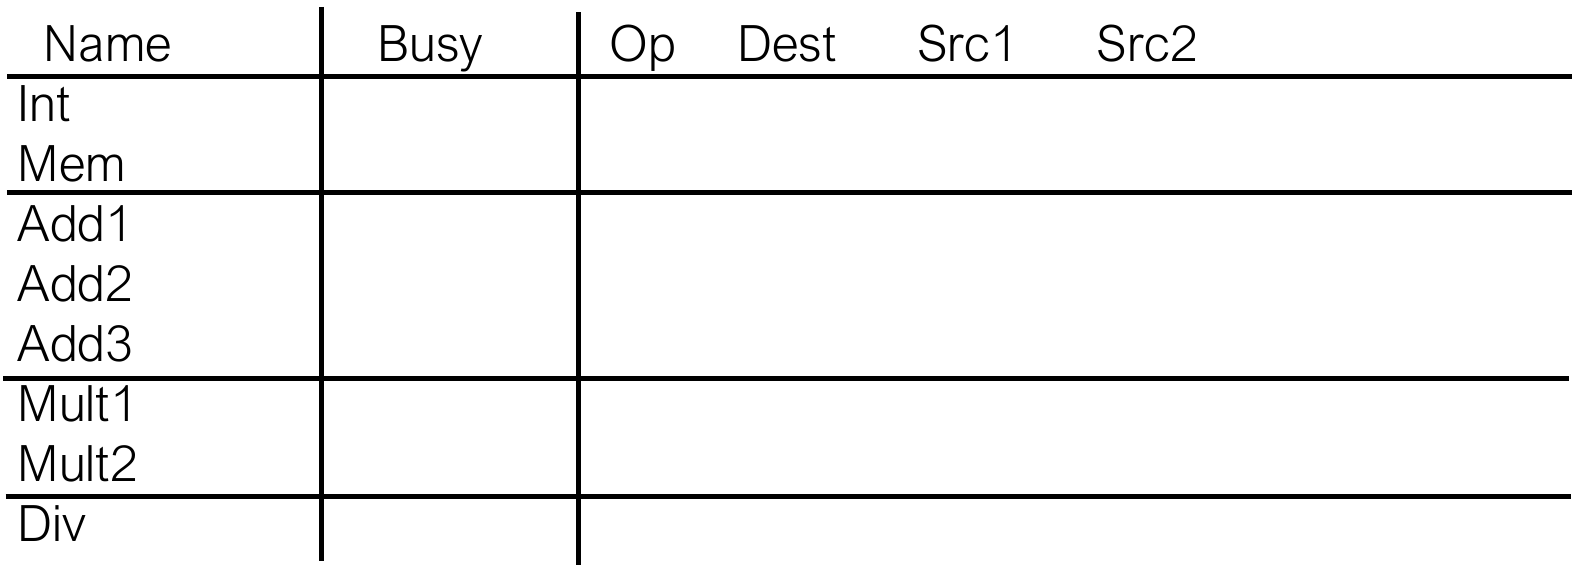
\includegraphics[scale=0.4]{Scoreboard_Table.png}
\end{figure}


The instruction i at the Issue stage consults this table
\begin{itemize}
  \item FU available? check the busy column
  \item RAW? search the dest column for i’s sources
  \item WAR? search the source columns for i’s destination
  \item WAW? search the dest column for i’s destination
\end{itemize}
An entry is added to the table if no hazard is detected;
An entry is removed from the table after Write-Back



\begin{figure}[htbp]
  \centering
  \tikzfig[1]{image-25.tikz}
  \caption{Structure of the \textit{Scoreboard}}
  \label{fig:structure-of-scoreboard}
\end{figure}

\newpage

\paragraph{Four stages of Scoreboard Control}

The four stages of scoreboard control are:

\begin{itemize}
  \item \textbf{Issue}: instructions are decoded and \textbf{structural hazards} and \textbf{\textit{(WAW)}} are checked for
        \begin{itemize}
          \item instructions are issued in program order for hazard checking
          \item if the \textit{FU} for the instruction is free and no other active instruction has the same destination register, the scoreboard issues the instruction and updates its internal data structure
          \item if a structural or \textit{WAW} hazard exists, then the instruction issue stalls and no further instructions are issued until they are solved
        \end{itemize}
  \item \textbf{Read operands}: expiration of data hazards is awaited, then operands are read
        \begin{itemize}
          \item a source operand if available if no earlier issued active instruction will write it or a functional unit is writing its value into a register
          \item when the source operands are available, the scoreboard tells the \textit{FU} to proceed to read the operands from the registers and begin execution
          \item \textit{RAW} hazards are resolved dynamically, instructions could be sent out of order
          \item there's no data forwarding in this model
        \end{itemize}
  \item \textbf{Execution}: the \textit{FUs} operate on the data
        \begin{itemize}
          \item when the result is ready, the scoreboard it's notified
          \item the delays are characterized by \textbf{latency} and \textbf{initiation interval}
        \end{itemize}
  \item \textbf{Write result}: the execution is finished
        \begin{itemize}
          \item once the scoreboard is aware that the \textit{FU} has completed the execution, it \textbf{checks for \textit{WAR} hazards}
                \begin{itemize}
                  \item if no \textit{WAR} hazard is found, the result is written
                  \item otherwise, the execution is stalled
                \end{itemize}
          \item \textbf{issue} and \textbf{write} stages \textbf{can overlap} (in realtà non sono certo... forse dipende)
        \end{itemize}
\end{itemize}

\smallskip
This structure creates a few implications:

\begin{itemize}
  \item \textit{WAW} are \textbf{detected} \textit{(and the pipeline is stalled)} until the other instruction is completed
  \item There's \textbf{no register renaming}
  \item \textbf{Multiple instructions must be dispatched} in the execution phase, creating the need for multiple or pipelined execution units
  \item Scoreboard \textbf{keeps track of dependences} and the state of the operations
\end{itemize}

\begin{remarks}
  NON HO CAPITO: Perchè per le WAW stalliamo e non facciamo nemmeno la issue, mentre per le WAR posso eseguire e aspettare solo al WB?
\end{remarks}

\paragraph{Riassunto per esercizi:}

\begin{tabular}{|m{10.5em}|m{10.5em} | m{10.5em} | m{10.5em} |}
  \hline
  \multicolumn{1}{|c|}{ISSUE} & \multicolumn{1}{|c|}{READ OPERAND} & \multicolumn{1}{|c|}{EXE COMPLETE} & \multicolumn{1}{|c|}{WB}\\
  \hline 
  Decode instruction & Read operands & Operate on operands & Finish exec \\
  \hline 
  \begin{itemize}[left=0pt]
    \item Structural FUs check
    \item WAW checks 
  \end{itemize}
  & 
  \begin{itemize}[left=0pt]
    \item RAW checks;
    \item WAW checks if need to read 
  \end{itemize}
  &
  \begin{itemize}[left=0pt]
    \item Notify Scoreboard on completion 
  \end{itemize}
  &
  \begin{itemize}[left=0pt]
    \item WAR check;
    \item Struct check (FUs will hold results)
    \item ... 
  \end{itemize}
  \\
  \hline
\end{tabular}

\newpage

\subsubsection{Tomasulo algorithm}

The Tomasulo algorithm is a \textbf{dynamic} algorithm that allows execution to proceed in presence of dependences.

The key idea behind this algorithm is to \textbf{distribute} the control logic and the buffers within \textit{FUs}, as opposed to the scoreboard \textit{(in which the control logic is centralized)}.

The operand buffers are called \textbf{Reservation Stations} \textit{(RS)}:
each instruction is also an entry to a \textit{RS} and its operands are replaced by values or pointers \textit{(a technique known as \textbf{Implicit Register Renaming})} in order to avoid \textit{WAR} and \textit{RAW} hazards.

Results are then dispatched to other \textit{FUs} through a \textit{Common Data Bus}, communicating both the data and the source.
Finally, \texttt{LOAD} and \texttt{STORE} operations are treated as \textit{FUs}, as \textit{RS} are more complex than architectural registers to allow more compiler-level optimizations.

\paragraph{Structure of the Reservation Stations}
The Reservation Station is composed by \(5\) \textbf{fields}:

\begin{itemize}
  \item \texttt{TAG} - indicating the \textit{RS} itself
  \item \texttt{OP} - the operation to perform in the unit
  \item \texttt{Vj}, \texttt{Vk} - the value of the source operands
  \item \texttt{Qj}, \texttt{Qk} - pointers to the \textit{RS} that produces \texttt{Vj}, \texttt{Vk}
        \begin{itemize}
          \item its value is zero if the source operator is already available in \texttt{Vj} or \texttt{Vk}
        \end{itemize}
  \item \texttt{BUSY} - indicates the \textit{RS} is busy
\end{itemize}

In this description, only one between the \texttt{V}-field and the \texttt{Q}-field is valid for each operand.

\medskip
Furthermore, a few more components are needed, such as:

\begin{itemize}
  \item \textbf{Register File} and the \textbf{Store} buffers have a \textit{Value} (\texttt{V}) and a \textit{Pointer} (\texttt{Q}) field
        \begin{itemize}
          \item \texttt{Q} corresponds to the number of the \textit{RS} producing the result (\texttt{V}) to be stored in \textit{Register File} or \textit{Store} buffers
          \item if \texttt{Q = 0}, no active instructions is producing a result and the \textit{Register File} \textit{(or \texttt{STORE})} buffer contains the wrong value
        \end{itemize}
  \item \textbf{Load} and \textbf{Store} buffers have an \textit{Address} (\texttt{A}) field, with the former having also a \textit{Busy} field \textit{(\texttt{BUSY})}
        \begin{itemize}
          \item the \texttt{A} field holds information for memory address calculation: initially contains the instruction offset, while after the calculation it stores the effective address
        \end{itemize}
\end{itemize}

\paragraph{Stages of the Tomasulo Algorithm}

The Tomasulo algorithm is structured in \(3\) different stages: \textbf{Issue}, \textbf{Execute} and \textbf{Write}. In more detail:

\begin{enumerate}
  \item \textbf{Issue} stage:
        \begin{itemize}
          \item Get an instruction \texttt{I} from the queue
                \begin{itemize}
                  \item if it is an \textit{FP} operation, check if any \textit{RS} in empty \textit{(i.e. check for any structural hazard)}
                \end{itemize}
          \item Rename the registers
          \item Resolve \textit{WAR} hazards
                \begin{itemize}
                  \item if \texttt{I} writes \textit{R}, read by an already issued instruction \texttt{K}, \texttt{K} will already know the value of \textit{R} or knows that instruction will write into it
                  \item the \textit{Register File} can be linked to \texttt{I}
                \end{itemize}
          \item Resolve \textit{WAW} hazards
                \begin{itemize}
                  \item since the in-order issue is used, the \textit{Register File} can be linked to \texttt{I}
                \end{itemize}
        \end{itemize}
  \item \textbf{Execute} stage:
        \begin{itemize}
          \item When both the operands are ready, then the operation is executed. Otherwise, watch the \textit{Common Data Bus} for results.
                \begin{itemize}
                  \item by delaying the execution until both operands are available, \textit{RAW} hazards are avoided
                  \item several instructions could become ready in the same clock cycle for the same \textit{FU}
                \end{itemize}
          \item \texttt{LOAD} and \texttt{STORE} are two-step processes:
                \begin{itemize}
                  \item effective address is computed and placed in \texttt{LOAD/STORE} buffer
                  \item \texttt{LOAD} operations are executed as soon as the memory unit is available
                  \item \texttt{STORE} operations wait for the value to be stored before sending it into the memory unit
                \end{itemize}
        \end{itemize}
  \item \textbf{Write} stage:
        \begin{itemize}
          \item When the result is available, it is written on the \textit{Common Data Bus}
                \begin{itemize}
                  \item it is then propagated into the \textit{Register File} and all the registers \textit{(including \texttt{STORE} buffers)} waiting for this result
                  \item \texttt{STORE} operations write data to memory
                  \item \textit{RSs} are marked as available
                \end{itemize}
        \end{itemize}
\end{enumerate}

\paragraph{Focus on \texttt{LOAD} and \texttt{STORE} in Tomasulo Algorithm}

\texttt{LOAD} and \texttt{STORE} instructions go through a functional unit for effective computation before proceeding to their respective load and \texttt{STORE} buffers.
\texttt{LOAD} take a second execution step to access memory, then go to \textit{Write} stage to send the value from memory to \textit{Register File} and/or \textit{RS}, while \texttt{STORE} complete their execution in their \textit{Write} stage.
All write operations occur in the write stage, thus simplifying the algorithm.

\bigskip
A \texttt{LOAD} and a \texttt{STORE} instruction can be done in a different order, provided they access different memory locations.
Otherwise, a \textit{WAR} \textit{(interchange in load-store sequence)} or a \textit{RAW} \textit{(interchange in store-load sequence)} may result in a  \textit{WAW} \textit{(if two stores are interchanged)}.
However, \texttt{LOAD} instructions can be reordered freely.

To detect such hazards, data memory addresses associated with any earlier memory operation must have been computed by the \textit{CPU}.

\bigskip
\texttt{LOAD} instructions executed out of order with previous \texttt{STORE} assume that the address is computed in program order.
When the \texttt{LOAD} address has been computed, it can be compared with \texttt{A} fields in active \texttt{STORE} Buffers: in case of a match, the load is not sent to its buffer until conflicting \texttt{STORE} completes.

Store instructions must check for matching addresses in both \texttt{LOAD} and \texttt{STORE} buffers.
This is a \textbf{dynamic disambiguation} and, opposing to the static disambiguation, is not performed by the compiler.
As a drawback, more hardware is required to perform these operations: each \textit{RS} must contain a fast associative buffer, because single \textit{CDB} \textit{(Common Data Bus)}  may limit performance.

\paragraph{Tomasulo and Loops}

Tomasulo algorithm can \textbf{overlap} iterations of loops due to:

\begin{itemize}
  \item \textbf{Register Renaming}
        \begin{itemize}
          \item \textbf{multiple iterations} use \textbf{different physical destinations} for registers
          \item \textbf{static register names are replaced} from code with dynamic registers \textit{"pointers"}, effectively increasing the size of the register file
          \item \textbf{instruction issue is advanced} past integer control flow operations
        \end{itemize}
  \item \textbf{Fast branch resolution}
        \begin{itemize}
          \item integer unit must \textit{"get ahead"} of floating point unit so that multiple iterations can be issued
        \end{itemize}
\end{itemize}

\paragraph{Comparison between Tomasulo Algorithm and Scoreboard}

The main advantages of the Tomasulo algorithm over the scoreboard are:

\begin{itemize}
  \item Control and buffers are \textbf{distributed} with \textit{FUs}
        \begin{itemize}
          \item \textit{FUs} buffers are called \textbf{reservation stations} and have pending operands
        \end{itemize}
  \item Registers in instructions are \textbf{replaced} by values or pointers to \textit{RS}
        \begin{itemize}
          \item avoids \textit{WAR} and \textit{WAW} hazards
          \item since there are more \textit{RS} than registers, there's a higher optimization than compilers alone can do
        \end{itemize}
  \item The result are \textbf{propagated} from \textit{RS} to \textit{FU} via \textit{Common Data Bus}
        \begin{itemize}
          \item the value is propagated \textbf{to all \textit{FUs}}
        \end{itemize}
  \item \texttt{LOAD} and \texttt{STORE} instructions are treated as \textit{FUs} with \textit{RSs}
  \item Integer instructions can go past \textbf{branches}, allowing \textit{FP} ops beyond basic block in \textit{FP} queue
\end{itemize}

\subsection{Limits of \textit{ILP}}

In order to execute more than one instruction at the beginning of a clock cycle, two requirements must be satisfied:

\begin{enumerate}
  \item Fetching more than one \textbf{instruction per clock cycle}
        \begin{itemize}
          \item this task is completed by the \textit{Fetch Unit}
          \item there is no major problem provided the instruction cache \textit{(I-cache)} can sustain the bandwidth and can manage multiple requests at one
        \end{itemize}
  \item Decide on data and control \textbf{dependences}
        \begin{itemize}
          \item \textit{dynamic scheduling} and \textit{dynamic branch prediction} are needed
        \end{itemize}
\end{enumerate}

Superscalar architectures paired with compiler scheduling can achieve such speeds.

\bigskip
A few requirements must be satisfied to start an ideal machine:

\begin{enumerate}
  \item \textbf{Register renaming}
        \begin{itemize}
          \item by using an infinite number of virtual registers, all \textit{WAW} and \textit{WAR} hazards are avoided
        \end{itemize}
  \item \textbf{Branch prediction}
        \begin{itemize}
          \item by using a perfect predictor, no branch is ever mispredicted
        \end{itemize}
  \item \textbf{Jump prediction}
        \begin{itemize}
          \item all jumps are perfectly predicted
          \item a machine with perfect speculation and an infinite buffer of instructions is needed
        \end{itemize}
  \item \textbf{Memory address alias analysis}
        \begin{itemize}
          \item addresses are known and a \texttt{STORE} can be moved before a \texttt{LOAD} if their addresses are different
        \end{itemize}
  \item \textbf{\(1\) cycle latency} for all instructions
        \begin{itemize}
          \item an unlimited number of instructions can be issued each clock cycle
        \end{itemize}
\end{enumerate}

\subsubsection{Initial assumptions}

Furthermore, a few \textbf{initial assumptions} must be made:

\begin{itemize}
  \item \textit{CPU} can issue an\textbf{ unlimited number of instructions}, looking arbitrarily far ahead in the computation
  \item There's \textbf{no restriction on types of instructions} that can be executed in one cycle \textit{(including loads and stores)}
  \item All \textit{FUs} \textbf{have unitary latency}: any sequence of depending instructions can issue on successive cycles
  \item All \textit{LOAD} and \textit{STORE} execute in \(1\) cycle, thanks to perfect caches
\end{itemize}

\subsubsection{Limits dynamic analysis}

\textbf{Dynamic analysis} is necessary to approach perfect branch prediction, and it cannot be achieved at compile time.
A perfect dynamic scheduled \textit{CPU} should:

\begin{enumerate}
  \item \textbf{Look arbitrarily far ahead} to find a set of instructions to issue and predict all branches perfectly
  \item \textbf{Rename all registers} in use, avoiding all \textit{WAR} and \textit{RAW} hazards
  \item Determine whether there are \textbf{data dependences among instructions} in the issue packet, renaming them if necessary
  \item Determine and handle all \textbf{memory dependences among issuing instructions}
  \item \textbf{Provide} enough replicated \textbf{functional units} to allow all ready instructions to issue
\end{enumerate}

\subsubsection{Limits on window size}

The size of the window size affects the number of comparisons needed to determine \textit{RAW} dependences.
The number of comparisons that are needed with the infinite register is:
\[ \displaystyle 2 \sum^{n-1}_{i=1} i = 2 \cdot \dfrac{(n-1)n}{2} = n^2 - n \]

For a window size of \(2000\) almost \textbf{\(4\) million comparisons} are needed;
a more realistic window with a size of \(50\) instructions still needs \(2450\) comparisons.

Today's \textit{CPUs} have constraints deriving from the limited number of registers, the search for dependent instructions and the in-order instructions issue.

\subsubsection{Other limits of modern \textit{CPUs}}

\begin{itemize}
  \item \textbf{Number} of \textit{FUs}
  \item \textbf{Number} of \textit{buses}
  \item \textbf{Number} of \textbf{ports} for the register file
\end{itemize}

All these limitations impose that the maximum number of instructions that can be issued, executed or committed in the same clock cycle is much smaller than the window size.

In real life, the maximum size of the issue width is capped at \(6\).
Increasing the issue rate above this value \textit{(i.e. at \(12\))} would require the \textit{CPU} to:
\begin{itemize}
  \item \textbf{Issue} \(3\) or \(4\) data memory accesses per cycle
  \item \textbf{Resolve} \(2\) or \(3\) branches per cycle
  \item \textbf{Rename} and access more than \(20\) registers per cycle
  \item \textbf{Fetch} between \(12\) and \(24\) instructions per cycle
\end{itemize}

The complexities of implementing these capabilities are likely to mean sacrifices in the maximum clock rate:
power consumption is nowadays an issue and it would grow too much.

The key question to answer is whether a technique is \textbf{energy efficient} enough:

\indentquote{Does it increase power consumption faster than it increases performances?}

Multiple issue processors techniques are all energy \textbf{inefficient}, as:

\begin{itemize}
  \item Issuing multiple instructions incurs some overhead in logic that grows faster than the issue rate grows
  \item A growing gap between peak issue rates and sustained performance is introduced, increasing energy per performance ratio
\end{itemize}

\subsection{Static Scheduling}

Compilers can use sophisticated algorithms for code scheduling to exploit \textit{ILP}.
The amount of parallelism available within a basic block \textit{(a straight line code sequence with no branches in except to the entry and no branches out except at the exit)} is quite small, and
data dependence can further limit the amount of \textit{ILP} that can be exploited within a basic block much less than the average basic block size.
To obtain substantial performance enhancements, \textit{ILP} must be exploited across multiple basic blocks \textit{(i.e. across branches)}.

The static detection and resolution of dependencies are accomplished by the compiler, so they are avoided by code reordering.
The compiler outputs dependency-free code.

\bigskip
\textbf{Limits of static scheduling}:
\begin{itemize}
  \item \textbf{Unpredictable} branches
  \item Variable memory \textbf{latency} \textit{(due to unpredictable cache misses)}
  \item Huge increase in \textbf{code size}
  \item High compiler \textbf{complexity}
\end{itemize}

\newpage

\subsection{VLIW architectures}

\begin{remarks}
  Lo scopo è sempre aumentare ILP (obbiettivo CPI < 1) in questo caso lo facciamo con una tecnica statica, sofware
\end{remarks}

The \textbf{Very Long Instruction Words} \textit{(VLIW)} is a particular architecture made specifically to fetch more instructions at a time.
The \textit{CPU} issues multiple sets of operations \textit{(single unit of computations, such as \texttt{ADD}, \texttt{LOAD}, \texttt{branch}, \ldots) }called \textbf{instructions}.
Those are meant to be intended to be issued at the same time and the compiler has to specify them completely.


Operation vs instruction:
\begin{definition}
  Operation: is a unit of computation (add, load,
branch = instruction in sequential ar.)  
\end{definition}

\begin{definition} \textbf{Instruction:} set of operations that are intended to be issued simultaneously  
\end{definition}

\begin{remarks} \hfill
  \begin{itemize}
    \item Compiler decides which operation to go to each instruction (scheduling)
    \item All operations that are supposed to begin at the same time are packaged into a single
    VLIW instruction
    \item We don't issue multiple istructions, we issue a single instruction (so we a single PC) very complex because is composed of mulitple operation.
  \end{itemize} 
\end{remarks}

\begin{remarks}
  Till now was the architecture that do everything for us: deals with hazards ecc\dots 
  Now all is up to compiler, our hardware is stupid. The compiler has to guarantee the dependences free code, because otherwise our simpler architecture is not able to deal with those hazards.
  Now there is the problem of binary compatibility:   
\end{remarks}

\smallskip
Its features include:

\begin{itemize}
  \item \textbf{Fixed number} of instructions \textit{(between \(4\) and \(16\))}
  \item The instructions are scheduled by the \textbf{compiler}
        \begin{itemize}
          \item the hardware has \textbf{very limited control} on what is going on
          \item the instructions are going to have a \textbf{very low dependency}
        \end{itemize}
  \item The operations are put into wide \textbf{templates}
  \item \textbf{Explicit} parallelism
        \begin{itemize}
          \item parallelism is found at compile time, not run time
          \item the compiler is responsible for parallelizing the code, not the designer
        \end{itemize}
  \item Single \textbf{control flow}
        \begin{itemize}
          \item there's only one \texttt{PC}
          \item only one instruction is issued each clock cycle
        \end{itemize}
  \item Low hardware \textbf{complexity}
        \begin{itemize}
          \item there's no need to to perform \textit{scheduling} or \textit{reordering} on hardware level
          \item all operations that are supposed to begin at the same time are packaged into a single instruction
          \item each operations slot is meant for a fixed functions
          \item constant operation latencies are specified
        \end{itemize}
\end{itemize}

There are multiple \textbf{functional units} \textit{(FUs)} that are going to execute instructions in parallel.
An illustration of the inner working instruction level is represented in Figure~\ref{fig:vliw-instruction-level}, while the pipeline level is represented in Figure~\ref{fig:vliw-pipeline-level}.

\newpage

\begin{figure}[htbp]
  \centering
  \tikzfig[1]{image-26.tikz}
  \caption{\textit{VLIW} - instructions level}
  \label{fig:vliw-instruction-level}
\end{figure}

\begin{itemize}
  \item Multiple operations packed into one instruction
  \item Each operation slot is for a fixed function
  \item Constant operation latencies are specified
  \item Architecture requires guarantee of:
  \begin{itemize}
    \item Parallelism within an instruction => no x-operation RAW check
    \item No data use before data ready => no data interlocks
  \end{itemize}
\end{itemize}

In this exampmle we can deal 2 integer op, 2 memory op, 2 floating point op.

We have to guaratee that those operations, scheduled in this VLIW hasn't conflict and no any dependences among those instructions.
All that dependeces are solved by the compiler. 

\begin{figure}[htbp]
  \bigskip
  \centering
  \tikzfig[1]{image-27.tikz}
  \caption{\textit{VLIW} - pipeline level}
  \label{fig:vliw-pipeline-level}
  \bigskip
\end{figure}

Note that in the complex pipeline we have multiple functional unit but the issue phase was blocking us in making one issue at the time $\to$ single issue architecture
VLIW is not a a proper multiple issue, but the point  that we are exectiting in paralled multiple operations. 

\medskip

But... Is it always possible schedule 6 kind of operations completely in parallel? No... dependes on the code. Dependeces are big problems for that kind of architecture.

\newpage

\subsubsection{Compiler responsibilities: what the compiler has to do}

The \textbf{compiler} has to schedule the instructions \textit{(via \textbf{static scheduling})} to maximize the parallel execution:

\begin{itemize}
  \item It can exploit \textit{ILP} and \textit{LLP} \textit{(Loop Level Parallelism)}
  \item It is necessary to \textbf{map the instructions} over the machine functional units
  \item This mapping must account for \textbf{time constraints and dependences} among the tasks themselves
\end{itemize}

The idea behind the static scheduling in \textit{VLIW} is to utilize all functional units \textit{(FUs)} in each cycle as much as possible to reach a better \textit{ILP} and therefore higher parallel speedups.

\subsubsection{Basic Blocks and Trace Scheduling}
\label{sec:trace-scheduling}

Compilers use sophisticated algorithms to schedule code and exploit \textit{ILP}.
However, the amount of parallelism available in a single \textbf{basic block}, as previously pointed out, is quite small; furthermore, \textbf{data dependence} can limit the amount of \textit{ILP} that can be exploited to less than the average block size.

\begin{definition}
  \textbf{Basic block \textit{(BB)}:}  sequence of straight non-branch instructions, that are for sure, serially exectuted.
\end{definition}

\begin{definition} \textbf{Trace:} 
  \begin{itemize}
    \item is a \textbf{loop-free sequence} of basic blocks
  embedded in the control flow graph (Fisher). It can include branches.
    \item is an \textbf{execution path} which can be taken for some
    set of inputs
    \item The chances that a trace is actually executed
    depends on the input set that allows its execution
  \end{itemize}
  \textbf{Some} traces are executed \textbf{much more frequently} than others (think about code inside loops).
  \label{def:trace}
\end{definition}

The tracing scheduling algorithm works as follows:

\begin{enumerate}
  \item Pick a \textbf{sequence of basic blocks} that represents the most frequent branch path
  \item Use \textbf{profiling feedback} or compiler heuristics to find the common branch paths
  \item \textbf{Schedule} the whole trace at once
  \item Add \textbf{code to handle branches} jumping out of trace
\end{enumerate}

Scheduling in a trace relies on basic code motion but it could also use globally scoped code by appropriately \textit{renaming} some blocks.
Compensation codes are then needed for \textbf{side entry points} \textit{(i.e. points except beginning)} and \textbf{slide exit points} \textit{(i.e. points except the ending)}.

Blocks on non-common paths may now have added overhead, so there must be a high probability of taking common paths according to the profile.
However, this choice might not be clear for some programs.

In general, compensation codes are not easy to generate for entry points.

\smallskip
A comparison of scheduled and unscheduled codes can be found in Figure~\ref{fig:compare-scheduled-unscheduled-code}.

\begin{figure}[htbp]
  \centering

  \begin{subfigure}[b]{0.495\textwidth}
    \centering
    \tikzfig[0.8]{image-28.tikz}
    \caption{Basic blocks}
    \label{fig:basic-blocks}
  \end{subfigure}
  \begin{subfigure}[b]{0.495\textwidth}
    \centering
    \tikzfig[0.8]{image-29.tikz}
    \caption{Trace scheduled code}
    \label{fig:trace-scheduled-code}
  \end{subfigure}
  \caption{Comparison of scheduled and unscheduled code}
  \label{fig:compare-scheduled-unscheduled-code}
\end{figure}

\newpage

\subsubsection{Pros and cons of \textit{VLIW}}

\textit{Pros}:
\begin{itemize}[label=\cmarkthin]
  \item \textbf{Simple} \textit{HW} ($\to$ energy-saving)
  \item It's \textbf{easy} to increase the number of FU
  \item Good \textbf{compilers} can efficiently \textbf{detect parallelism}
\end{itemize}

\bigskip
\textit{Cons}:
\begin{itemize}[label=\xmarkthin]
  \item \textbf{Huge number of registers }to keep active each FU, each needed to store operands and results
  \item \textbf{Large data transport} capabilities between:
        \begin{itemize}
          \item FUs and register files
          \item register files and memory
        \end{itemize}
  \item H\textbf{igh bandwidth} between instruction cache and fetch unit
  \item \textbf{Large code} size
\end{itemize}

\newpage

\subsubsection{Static Scheduling methods}

The static scheduling methods used in the \textit{VLIW} are:

\begin{itemize}
  \item Simple code \textbf{motion}
  \item \textbf{Loop unrolling} and loop peeling - \textit{Paragraph~\ref{par:loop-unrolling}}
  \item Software \textbf{pipelining} - \textit{Paragraph~\ref{par:software-pipelining}}
  \item Global code \textbf{scheduling} \textit{(across basic blocks)}
        \begin{itemize}
          \item \textbf{Trace} scheduling - \textit{Paragraph~\ref{par:trace-scheduling}}
          \item \textbf{Superblock} scheduling
          \item \textbf{Hyperblock} scheduling
          \item \textbf{Speculative} Trace scheduling
        \end{itemize}
\end{itemize}

\paragraph{Simple code motion}
\label{par:simple-code-motion}

We can reaschedule (move) part of our code from a portion of a program to another.   

\begin{figure}[!h]
  \centering
  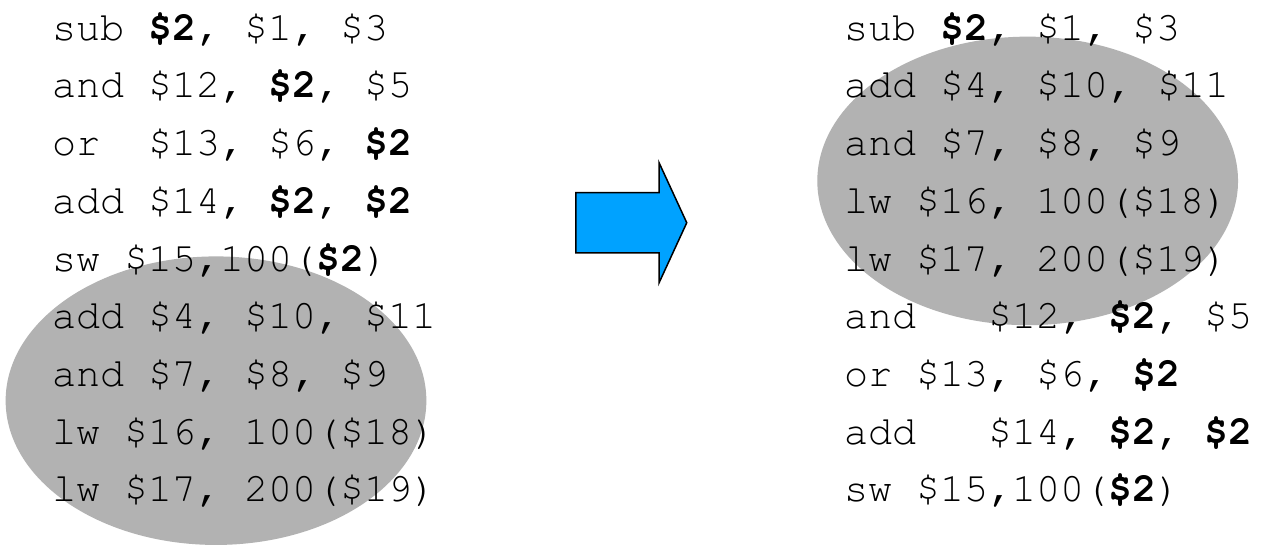
\includegraphics[scale=0.4]{Simple_Code_Motion.png}
\end{figure}

\paragraph{Loop unrolling}
\label{par:loop-unrolling}

Examine this snippet of code:

\begin{verbatim}
  for (int i = 0; i < N; i++)
    B[i] = A[i] + C;
\end{verbatim}

the inner loop gets \textit{unrolled} in order to execute \(4\) iterations at once:

\begin{verbatim}
  for (int i = 0; i < N; i += 4) {
    B[i] = A[i] + C;
    B[i + 1] = A[i + 1] + C;
    B[i + 2] = A[i + 2] + C;
    B[i + 3] = A[i + 3] + C;
  }
\end{verbatim}

The performance:

\begin{tabular}{m{22em} m{22em}}
  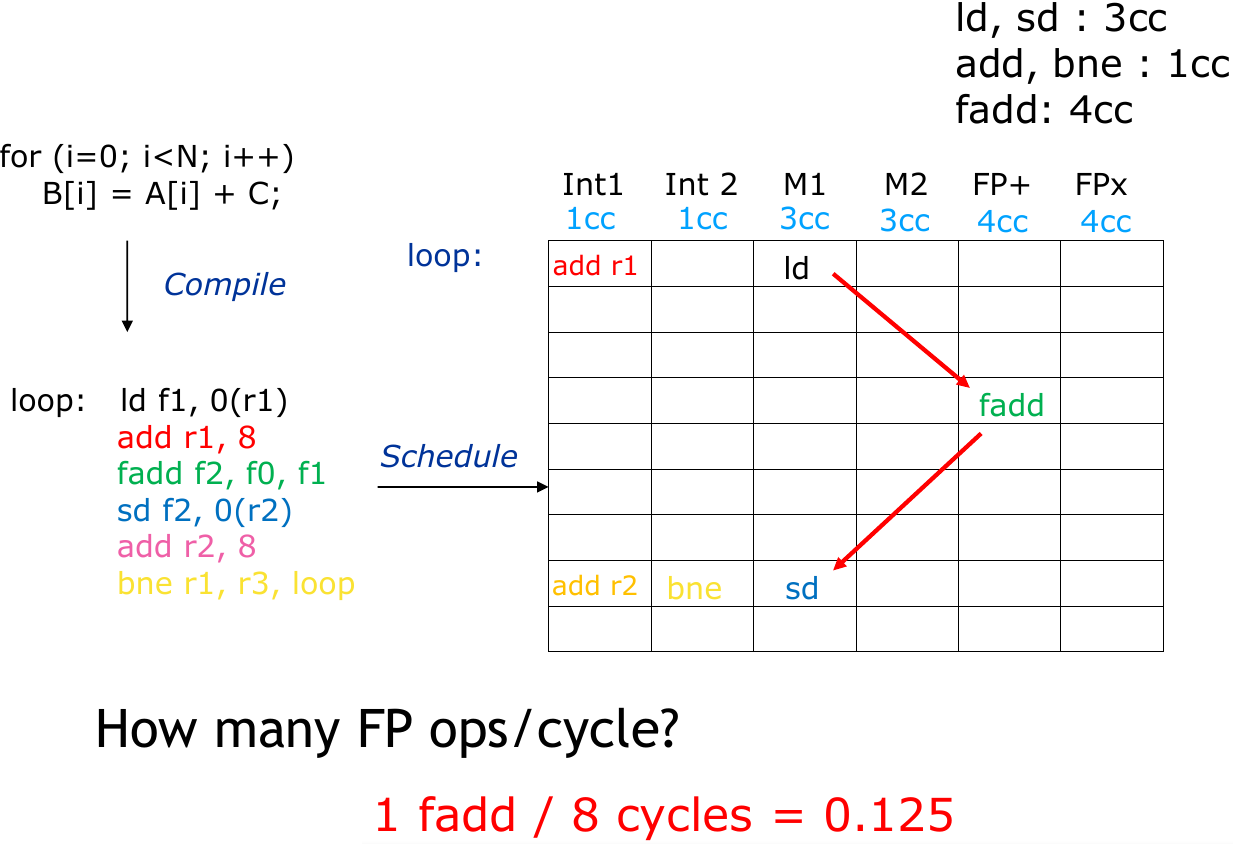
\includegraphics[scale=0.26]{Loop_execution.png}
  &
  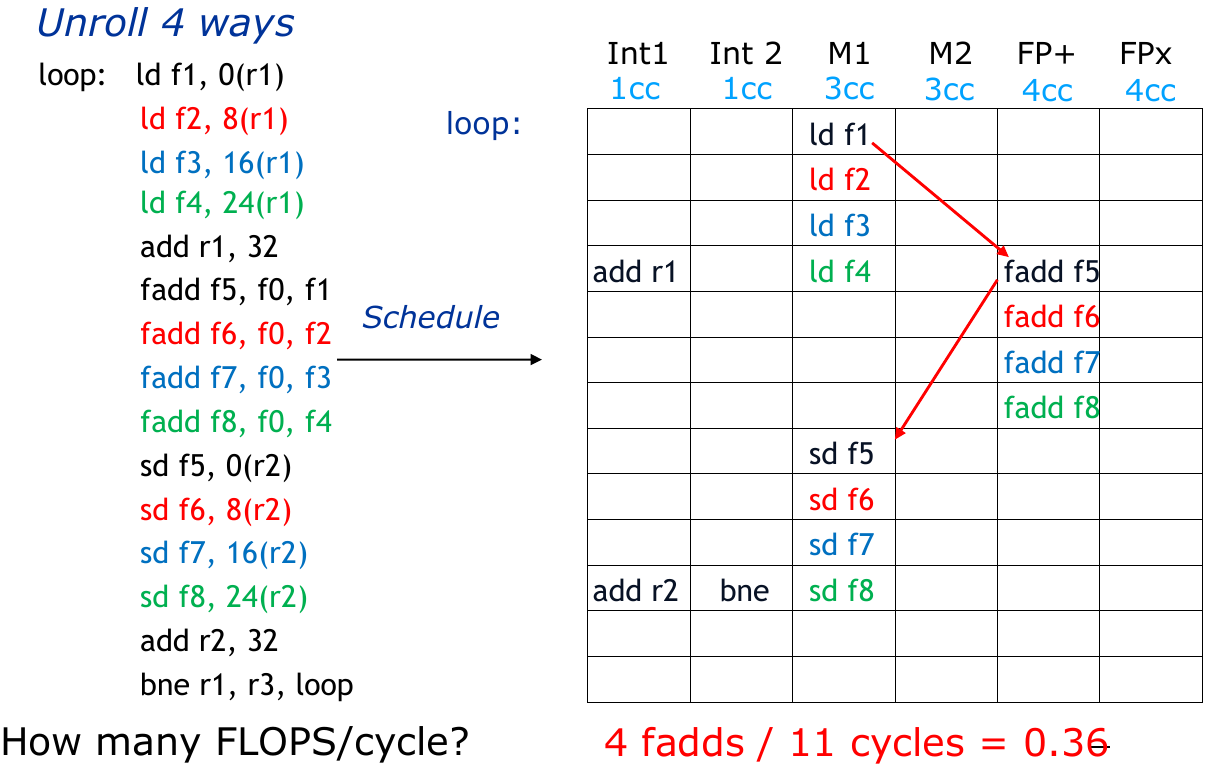
\includegraphics[scale=0.26]{Loop_exectution_with_unrolling.png}
\end{tabular}

\begin{remarks}
  NOTA (HAI UN DUBBIO): Why in the unrolled version we didn't put \textit{ld F2} in the M2 in the same cc of \textit{ld F2}? 
  \begin{itemize}
    \item preserve structure (very very important)
    \item doesn't affect the performance (we have only one FU for FP+)
  \end{itemize}
\end{remarks}


A final clean-up is needed to take care of those values of \texttt{N} that are not multiples of the unrolling factor \textit{(\(4\) in this example)}.

This technique has the drawbacks of creating \textbf{longer code} and \textbf{losing performance} due to the costs of starting and closing each iteration (probably we can do better).
Furthermore, trace scheduling cannot proceed beyond a loop.

\bigskip
An illustration of the performance improvements can be found in Figure~\ref{fig:performance-improvement-loop-unrolling}.

\begin{figure}[htbp]
  \bigskip
  \centering
  \tikzfig[1]{image-31.tikz}
  \caption{Performance improvement of loop unrolling}
  \label{fig:performance-improvement-loop-unrolling}
  \bigskip
\end{figure}
 
\begin{remarks}
  Note this technique is useful only if you don't have \textbf{loop-carried-dependencies}.
\end{remarks}

\newpage

\paragraph{Software pipelining}
\label{par:software-pipelining}

\begin{remarks}
  In loop unrolling we execute the iterations serially, we can somehow pipeline the iteration. Overlap as much as you can.
\end{remarks}

\begin{figure}[!h]
  \centering
  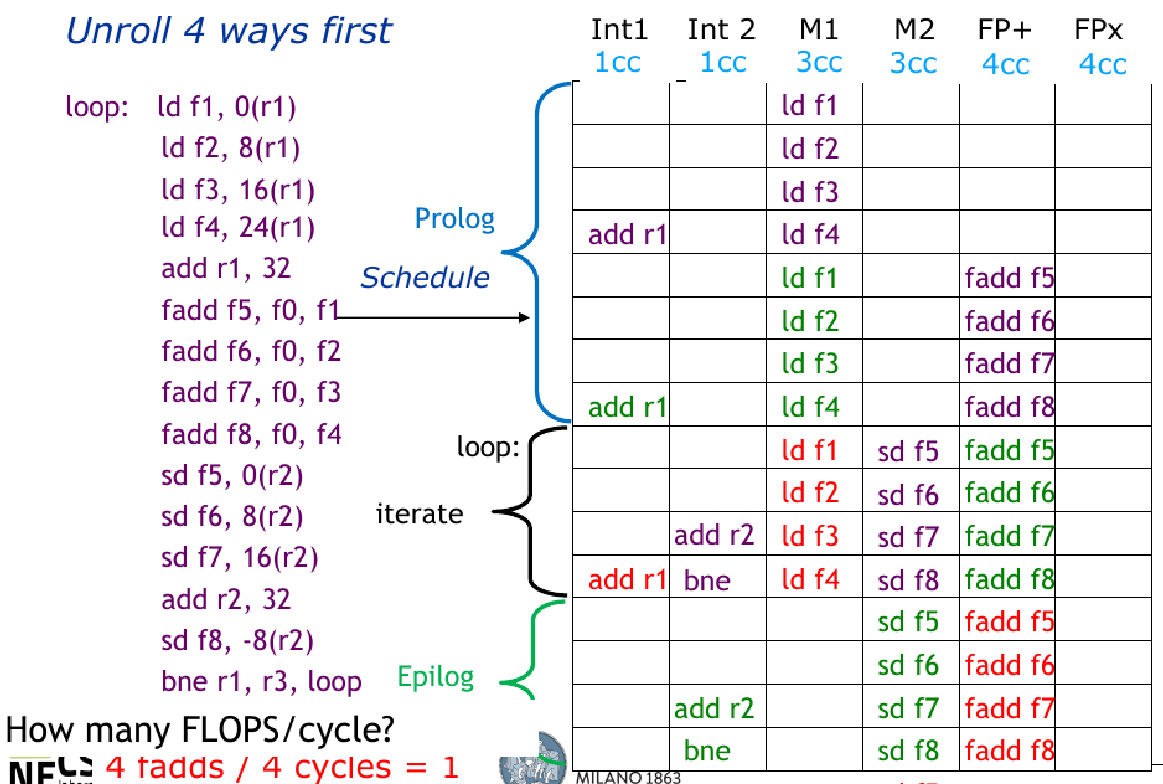
\includegraphics[scale=0.5]{Loop_execution_with_software _pipelining.png}
\end{figure}

The programs can be pipelined in order to increase performance and reduce the overall cost of the startup and wind down phases from once per iteration to once per loop.

\bigskip
An illustration of the performance improvements can be found in Figure~\ref{fig:performance-improvement-software-pipelining}.

\begin{figure}[htbp]
  \bigskip
  \centering
  \tikzfig[1]{image-32.tikz}
  \caption{Performance improvement of software pipelining}
  \label{fig:performance-improvement-software-pipelining}
  \bigskip
\end{figure}

\newpage

\paragraph{Trace scheduling}
\label{par:trace-scheduling}

\begin{remarks}
  NON CI SARANNO ESERCIZI SU QUESTA PARTE (SANTAMBROGIO). E devi dire la verità, non ho capito bene.
\end{remarks}

Now we need something in case we don't have loops. Trace Scheduling is what we need, in fact it does not support loops.

\medskip

Trace scheduling focuses on \textit{\hyperref[def:trace]{trace}}. The basic steps are:

\begin{enumerate}
  \item Pick a trace that is most frequent branch path
  \item Use profiling feedback, benchmarks, profiling to find most frequent branch paths
  \begin{itemize}
    \item Traces scheduling schedules traces in order of
    decreasing probability of being executed
    \begin{itemize}
      \item So, most frequently executed traces get better schedules
      \item Traces are scheduled as if they were basic blocks (no special considerations for branches)   
    \end{itemize}
  \end{itemize}
  \item Schedule whole “trace” at once 
  \item Add fixup code to cope with branches jumping out of trace
\end{enumerate}

What if we meet a loop?
\begin{itemize}
  \item Trace scheduling cannot proceed beyond a loop barrier
  \item Techniques used to overcome this limitation are based on
  loop unrolling. Negative effects on unrolling:
  \begin{itemize}
    \item Unrolling produces much extra code
    \item It also looses performance, because of the costs of starting
    and closing the iterations  
  \end{itemize}
\end{itemize}
 
\medskip

Scheduling in a trace rely on basic code motion but now
has a global taste across more that one basic block by
appropriate use of renaming (NON HO CAPITO QUESTA FRASE)

\smallskip

\textbf{Compensation codes are needed:}
\begin{itemize}
  \item for side entry points: i.e. points except beginning
  \item and slide exit points: i.e. points except ending  
\end{itemize}
Blocks on non common path may now have added
overhead, so there must be a high probability of taking
common path according to profile (may not be clear for
some programs)

\smallskip

Problems: compensation codes are difficult to generate
specially for entry points

\begin{example} \textbf{Trace Scheduling} \hfill \break
  For example suppose that B1,B3,B4,B5,B7 is the most frequently executed path
  
  \begin{tabular}{m{22em} m{22em}}
    Therefore traces are
    \begin{itemize}
      \item B1,B3
      \item B4
      \item B5,B7
    \end{itemize}
    Remember that a Trace is a sequence of BB without loops. But B4 is a loop, so the trace have to be divided in that way.
    
    \medskip

    \textbf{Eache trace is scheduled independently}
    &
    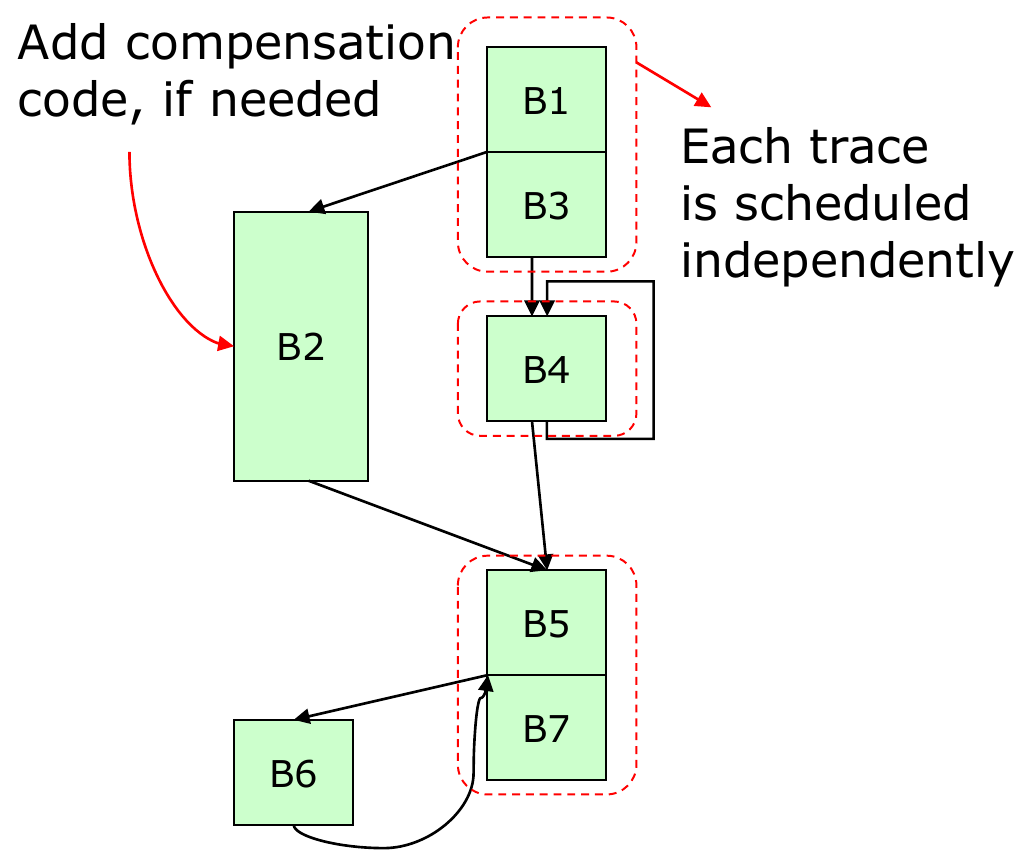
\includegraphics[scale=0.25]{Trace_Scheduling_Example.png}  
  \end{tabular}
\end{example}

\begin{remarks} \textbf{Perchè spostare le istruzioni nel VLIW?}
  Magari in un ciclo di VLIW hai esaurito lo spazio per le integer operation ma ne avresti ancora altre da eseguire.
  Allora puoi spostarla avanti per eseguirla successivamente e magari quindi anticipare un operazione di floating point 
  nel caso ci sia ancora posto nella VLIW.
\end{remarks}

\begin{example} \textbf{Trace Scheduling Compensation 1} \hfill \break
  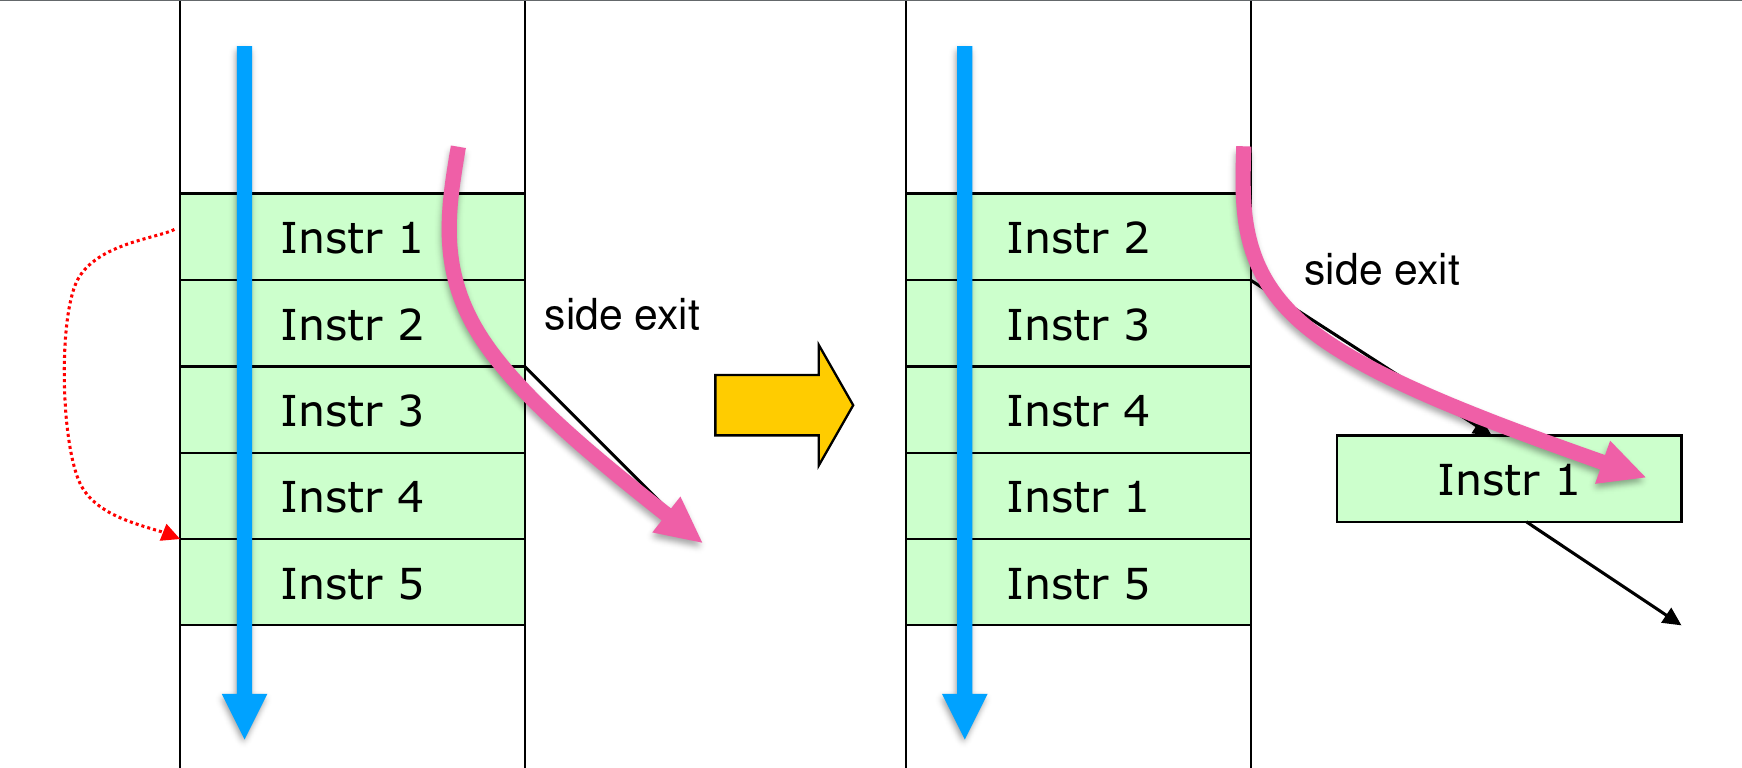
\includegraphics[scale=0.3]{Trace_Scheduling_Compensation_1.png}
\end{example}

\begin{example} \textbf{Trace Scheduling Compensation 2} \hfill \break
  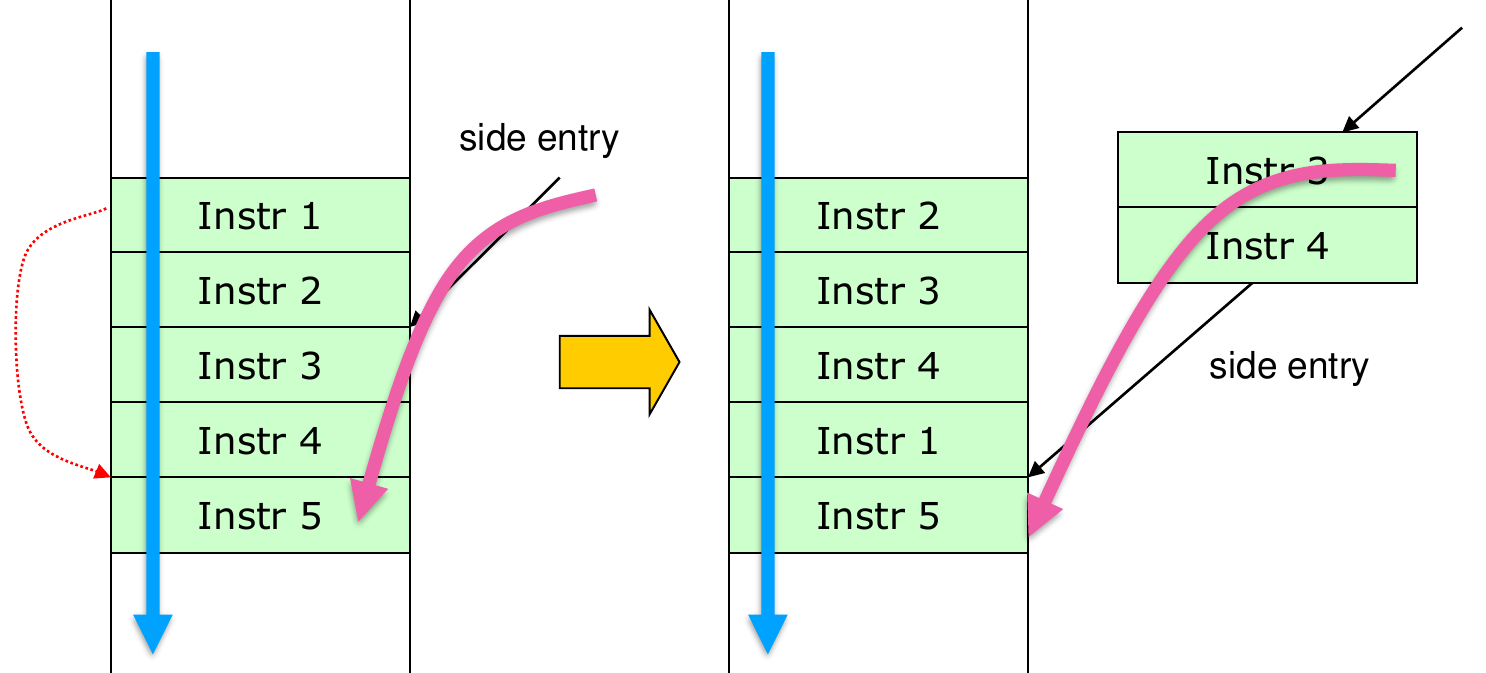
\includegraphics[scale=0.4]{Trace_Scheduling_Compensation_2.png}
\end{example}

\begin{remarks}
  Con questi due example potresti capire perchè si parla di \textbf{code explosion}. 
  Ma non influenzeranno effettivamente, perchè tu userai magari slot del VLIW che altrimenti sarebbero inutilizzati!
\end{remarks}

\paragraph{Code Motion in Trace Scheduling}

\begin{remarks}
  MOLTO MOLTO DIFFICILE E SPIAGATA MALE
\end{remarks}
In addition to need of compensation codes there are
restrictions on movement of a code in a trace:
\begin{itemize}
  \item The \textbf{dataflow} of the program must not change \\
  Dataflow can be guaranteed to be correct by maintaining two dependencies:
  \begin{itemize}
    \item Data dependency
    \item Control dependency \\ 
    There are two solutions to eliminate control dependency:
    \begin{itemize}
      \item By use of predicate instructions (Hyperblock scheduling) and
      removing the branch.
      \item By use of \textbf{speculative instructions (Speculative Scheduling)}
      and speculatively move an instruction before the branch. Magari metto un istruzione molto lunga che è dentro l'if, prima del branch, cosi ho due possibilità ho entro nell'if e il lavoro è ok, oppure vado nell'else e devo eliminare/dimeticare quella istruzione.
    \end{itemize} 
  \end{itemize}
  \item The \textbf{exception behavior} must be preserved
\end{itemize}





To increase the performance in these situations, techniques based on loop unrolling are needed.
Traces scheduling schedules traces in order of decreasing probability of being executed.
As such, the most frequently executed traces get better schedules.

\paragraph{Code motion and Rotating Register Files in Trace Scheduling}
\begin{remarks}
  Non ho visto fare questa parte
\end{remarks}

In addition to the need for compensation codes, there are a few more restrictions on the movement of a code trace:

\begin{enumerate}[label=\Alph*), ref=(\Alph*)]
  \item \label{enum:data-flow-trace-scheduling} The \textbf{data flow} of the program must not change
  \item \label{enum:exception-behaviour-trace-scheduling} The \textbf{exception behaviour} must be preserved
\end{enumerate}

\bigskip

In order to ensure \ref{enum:data-flow-trace-scheduling}, the \textbf{Data} and \textbf{Control} dependency must be maintained.
Furthermore, control dependency can be eliminated using \textbf{predicate instructions} \textit{(via Hyperblock scheduling) }and branch removal or by using \textbf{speculative instructions} \textit{(via Speculative Scheduling)} and speculatively moving instructions before branches.

Finally, Trace Scheduling within loops requires lots of registers, due to the duplicated code:
to solve this issue, a new set of registers must be allocated for each iteration.

This solution is achieved via the use of \textbf{Rotating Register Files} \textit{(RRB)}.
The address of the \textit{RRB} register points to the base of the current register set.
The value added onto a local register specifier gives a physical register number.

\bigskip
An illustration of the \textit{RRB} is shown in Figure~\ref{fig:rotating-register-file}.

\begin{figure}[htbp]
  \bigskip
  \centering
  \tikzfig[1]{image-30.tikz}
  \caption{Rotating Register File}
  \label{fig:rotating-register-file}
  \bigskip
\end{figure}


\clearpage

\section{Hardware Based Speculation}

The Hardware Based Speculation combines \(3\) ideas:

\begin{itemize}
  \item \textbf{Dynamic Branch Prediction} to choose which instruction to execute
  \item \textbf{Dynamic Scheduling} to support out-of-order execution while allowing in-order commit
        \begin{itemize}
          \item prevents irrevocable actions such as register update or exception taking until an instruction commits
        \end{itemize}
  \item \textbf{Speculation} to execute instructions before control dependencies are resolved
\end{itemize}

The outcome of the branches is speculated, and then the program is executed as if the speculation was correct.
Mechanisms are necessary to handle incorrect speculation: the hardware speculation extends dynamic scheduling beyond a branch \textit{(i.e. beyond the basic block)}.

\bigskip
Generally speaking, Hardware-Based Speculation raises power consumption but lowers execution time by more than it increases the average power consumption.
The total energy consumed may be less depending on the number of instructions incorrectly executed.

\subsection{Reorder Buffer}

The \textbf{Reorder Buffer} \textit{(\textit{ROB})} holds instructions in \textit{FIFO} order, exactly as issued:
when the instructions are complete, their results are placed back in the \textit{ROB}.

Operands are supplied to the other instructions between their completion and their commit, while results are tagged with \textit{ROB} buffer number instead of the reservation station.

During the instruction commit, the values in the head of the \textit{ROB} are placed in registers.

\bigskip
\textit{ROB} are structured as a circular buffer with \textbf{head} and \textbf{tail} pointers.
Entries between those two are valid and they are allocated and freed whenever an instruction enters or leaves the \textit{ROB}.

Its main entries are:

\begin{itemize}
  \item The \textbf{type} of the instruction
  \item The \textbf{destination} register of the result
  \item The \textbf{result} of the instruction
  \item If any \textbf{exception} was raised
  \item The \textbf{program counter} \texttt{PC}
  \item If the \textbf{instruction} is \textbf{ready}
  \item If the \textbf{branch} is \textbf{speculative}
\end{itemize}

\bigskip
The structure of the \textit{ROB} is represented in Figure~\ref{fig:structure-of-ROB} along with its main entries.

\begin{figure}[htpb]
  \bigskip
  \centering
  \begin{subfigure}[]{\textwidth}
    \centering
    \tikzfig[1]{image-33.tikz}
    \caption{\textit{ROB} structure}
    \label{subfig:structure-rob}
  \end{subfigure}
  \par\bigskip
  \begin{subfigure}[]{\textwidth}
    \centering
    \tikzfig[1]{image-34.tikz}
    \caption{\textit{ROB} entry}
    \label{subfig:rob-entries}
  \end{subfigure}
  \caption{Structure of the \textit{ROB} and its entries}
  \label{fig:structure-of-ROB}
  \bigskip
\end{figure}

\begin{minipage}{\textwidth}
  \bigskip
  The structure of an entry contains:

  \begin{itemize}
    \item The \texttt{TAG}, given by the index in the \textit{ROB}
    \item The new instructions are \textbf{dispatched} to free slot
    \item Instruction space is \textbf{reclaimed} when done by setting the \texttt{P} bit
    \item In \textbf{dispatch} stage:
          \begin{itemize}
            \item non-busy source operands are read from register files and copied to \texttt{SRC} fields where the \texttt{P} bit is set
            \item busy source operands copy \texttt{TAG} of producer and clear the \texttt{P} bit
            \item the \texttt{V} bit is set valid
          \end{itemize}
    \item In \textbf{issue} stage:
          \begin{itemize}
            \item the \texttt{I} bit is set valid
          \end{itemize}
    \item On \textbf{completion}:
          \begin{itemize}
            \item source tags are searched and the \texttt{P} bit is set
            \item result and \texttt{EXCEPTION} flags are written back to \textit{ROB}
          \end{itemize}
    \item On \textbf{commit}:
          \begin{itemize}
            \item \texttt{EXCEPTION} flags are checked
            \item \texttt{RESULT} is copied into register files
          \end{itemize}
    \item On \textbf{trap}:
          \begin{itemize}
            \item machine and \textit{ROB} are flushed
            \item \texttt{FREE} pointer is set as \texttt{OLDEST}
            \item the execution resumes from \texttt{HANDLER}
          \end{itemize}
  \end{itemize}
\end{minipage}

\bigskip
In order to separate the completion stage from the commit stage, the \textit{ROB} must hold register results from the former until the latter.

Each entry, allocated in program order during decode, holds:

\begin{itemize}
  \item The \textbf{type} of the instruction
  \item The \textbf{destination} register specifier and value \textit{(if any)}
  \item The \textbf{program counter}, \texttt{PC}
  \item The \textbf{exception} status \textit{(often compressed to save memory)}
\end{itemize}

They buffer completed values and exception states until the in-order commit point.
Completed values can be used by dependencies before reaching that point.

\subsection{Interrupts and Exceptions with hardware speculation}

Hardware Speculation greatly increases the complexity of control dependencies;
branch prediction may not be enough to keep a high level of \textit{ILP}.

Special care must be ensued while handling \textbf{interrupts} and \textbf{exceptions}, because:

\begin{itemize}
  \item All the instruction \textbf{before} the event must be completed
  \item All the instructions \textbf{after} the even must behave as they have never started
\end{itemize}

Since branch prediction might be wrong, the issue is now to update the processor state accordingly.
Finally, out-of-order completion, post-interrupt, and mispredict writebacks change the state of the program.

To solve this problem, executed instructions are held in \textit{ROB} until they are no longer speculative;
the instruction commit is then \textit{in order}: exceptions and interrupts are handled by not being addressed until the instruction that caused them is recorded in the \textit{ROB}.

Temporary storage \textit{(in the form of shadow registers and \texttt{STORE} buffers)} is then needed to hold all results before commit
Operands are supplied as well between execution completion and commit.

Once the instruction is committed, its result is placed in the destination register;
it's therefore easy to undo speculated instructions on exceptions and interrupts.

A scheme of this structure is represented in Figure~\ref{fig:exceptions-in-order-commit}.

\begin{figure}[htbp]
  \bigskip
  \centering
  \tikzfig[0.8]{image-35.tikz}
  \caption{Scheme of the in order commit for precise exceptions}
  \label{fig:exceptions-in-order-commit}
  \bigskip
\end{figure}

\subsection{Steps in the Speculative Tomasulo Algorithm}

The \(4\) steps of the Speculative Tomasulo Algorithm are:

\begin{enumerate}
  \item \textbf{Issue} or \textbf{dispatch} - instruction is loaded from \textit{FP} operation queue. If the reservation station and the reorder buffer slot are free, then:
        \begin{itemize}
          \item the instruction is issued
          \item the operands are sent
          \item the destination buffer is reordered
        \end{itemize}
  \item \textbf{Execution} - operands are operated upon
        \begin{itemize}
          \item when both operands are ready, the instruction is executed
          \item if they aren't, the \textit{Common Data Bus} is watched for the results
          \item when both operands are in the reservation station, the instruction is executed
          \item \textit{RAW} are checked
        \end{itemize}
  \item \textbf{Write result}
        \begin{itemize}
          \item result is written on the \textit{Common Data Bus} to all awaiting \textit{FUs} and \textit{ROBs}
          \item all the \textit{RS} are set to available
        \end{itemize}
  \item \textbf{Commit} or \textbf{graduation} - when the instruction at the head of the \textit{ROB} and the results are present, then:
        \begin{itemize}
          \item the register \textit{(or memory page)} is updated with the result
          \item the instruction is removed from the \textit{ROB}
          \item mispredicted branches are flushed from the \textit{ROB}
        \end{itemize}
\end{enumerate}

Furthermore, \(3\) possible \textbf{commit} sequences are possible:

\begin{itemize}
  \item \textbf{Normal commit}:
        \begin{itemize}
          \item the instruction reaches the head of the \textit{ROB}
          \item the result is found in the register
          \item the instruction is removed from the \textit{ROB}
        \end{itemize}
  \item \textbf{Store commit}:
        \begin{itemize}
          \item same as \textbf{Normal commit} but memory \textit{(and not a register)} is updated
        \end{itemize}
  \item \textbf{Instruction is a branch with incorrect prediction}:
        \begin{itemize}
          \item the speculation was wrong
          \item \textit{ROB} is flushed \textit{(the operation is called \inlinequote{graduation})}
          \item execution restarts at the correct successor of the branch
        \end{itemize}
\end{itemize}

\subsubsection{Tomasulo's Algorithm and \textit{ROB}}

Tomasulo's Algorithm needs a buffer for all the uncommitted results.
It's structured as a \textit{ROB}.

Each entry of the \textit{ROB} contains \(4\) fields:

\begin{enumerate}
  \item \textbf{Instruction Type} field, indicating if:
        \begin{itemize}
          \item the instruction is a \textit{branch} \textit{(and has no destination result)}
          \item the instruction is a \texttt{STORE} \textit{(and has a memory address destination)}
          \item the instruction is a \texttt{LOAD} or \textit{ALU} operation \textit{(and has a register destination)}
        \end{itemize}
  \item \textbf{Destination} field, supplying:
        \begin{itemize}
          \item the register number \textit{(for \texttt{LOAD} and \textit{ALU} instructions)}
          \item the memory address \textit{(for \texttt{STORE} instructions)}
        \end{itemize}
  \item \textbf{Value} field, holding the value of the result until the instruction commits
  \item \textbf{Ready} field, indicating if the instruction has been completed and the value is ready
\end{enumerate}

\bigskip
Further observations:

\begin{itemize}
  \item The \textit{ROB} replaces all store buffers, because \texttt{STORE} execute in two steps
        \begin{itemize}
          \item the second step happens when the instruction commits
        \end{itemize}
  \item The renaming function of the reservation stations is completely replaced by the \textit{ROB}
        \begin{itemize}
          \item Tomasulo provides \textbf{Implicit Registers Renaming}, because user registers are renamed to reservation station tags
        \end{itemize}
  \item Reservation stations now only queue operations \textit{(and their relative operands)} to \textit{FUs} between the time they issue and the time they begin their execution stage
  \item Results are tagged with the \textit{ROB} entry number rather than with the \textit{RS} number
        \begin{itemize}
          \item each \textit{ROB} assigned to instruction must be tracked in the \textit{RS}
        \end{itemize}
  \item All instructions \textbf{excluding incorrectly predicted branches} and \textbf{incorrectly speculated \texttt{LOAD}} commit when reaching head of \textit{ROB}
        \begin{itemize}
          \item when an incorrect prediction or speculation is indicated, the \textit{ROB} is flushed and execution restarts at the correct successor of branch
          \item speculative actions are easily undone
        \end{itemize}
  \item Processors with \textit{ROB} can dynamically execute while maintaining a precise interrupt model
        \begin{itemize}
          \item if instructions \(I\) causes an interrupt, the \textit{CPU} waits until \(I\) reaches the head of the \textit{ROB} to handle it, flushing all other pending instructions
        \end{itemize}
\end{itemize}

\subsubsection{Exception handling}

The use of a \textit{ROB} with in-order instruction commit provides precise exceptions:
they are handled by ignoring them until they are ready to commit.

3 different scenarios can then be identified in the commit stage:

\begin{itemize}
  \item If a \textbf{speculated instruction raises an exception}, then the exception itself is recorded in the \textit{ROB}
  \item If a \textbf{branch misprediction arises} and the instruction should not have been executed, then the exception is flushed along with the instruction when the \textit{ROB} is cleared
  \item If the \textbf{instruction reaches the head of the \textit{ROB}}, then it's no longer speculative and it should be addressed
\end{itemize}

\subsubsection{Hardware support for Memory Disambiguation}

In order to keep track of all stores to memory in program order, a buffer is needed.
Its duties include:

\begin{itemize}
  \item Keeping track of \textbf{addresses and results} and when they become available
  \item Keeping a \textbf{\textit{FIFO} ordering}, so stores are retired in program order
\end{itemize}

While issuing a \texttt{LOAD}, the current head of the \texttt{STORE} queue must be recorded to know which \texttt{STORE} instructions are ahead;
when the address is actually found, the \texttt{STORE} queue is checked:

\begin{itemize}
  \item If any \texttt{STORE} prior to \texttt{LOAD} is waiting for its address, \textbf{the \texttt{LOAD} is stalled}
  \item If any \texttt{LOAD} address matches any previous \texttt{STORE} address \textit{(found by associative lookup)}:
        \begin{itemize}[label=\(\rightarrow\)]
          \item a \textbf{memory induced} \textit{RAW} hazard is created
          \item if the \texttt{STORE} value is available, then it's returned
          \item if the \texttt{STORE} value is not available, then the \textit{ROB} number of the source is returned
        \end{itemize}
\end{itemize}

All the actual \texttt{STORE} instructions commit in order, so there's no need to check for \textit{WAR} or \textit{WAW} hazards throughout memory.

\subsection{Explicit Register Renaming}

\textbf{Explicit Register Renaming} is a technique that uses a physical register file that is larger than the number of registers specified by the \textit{ISA}.

The key \textit{idea} behind this technique is to allocate a new physical destination register for every instruction that writes;
it's very similar to a compiler transformation called \textbf{Static Single Assignment} \textit{(SSA)} but at hardware level.
It removes all chances of \textit{WAR} or \textit{WAW} hazards while allowing complete \textbf{out of order} completion.

It works by keeping a translation table that maps each \textit{ISA} register to a physical register:
whenever a register is written, the corresponding entry on the map is replaced with a new register from the \textbf{freelist}.
A physical register is considered free when not used by any active instruction.

A simple illustration of this technique is shown in Image~\ref{fig:explicit-register-renaming}.

\begin{figure}[htbp]
  \bigskip
  \centering
  \tikzfig[1]{image-36.tikz}
  \caption{Explicit Register Renaming}
  \label{fig:explicit-register-renaming}
  \bigskip
\end{figure}

Explicit Renaming Support includes:

\begin{itemize}
  \item \textbf{Rapid access} to a table of translations
  \item A physical register file that has \textbf{more registers} than specified by the \textit{ISA}
  \item Ability to figure out which physical registers are \textbf{free}
        \begin{itemize}
          \item if no register is free, the issue stage is stalled
        \end{itemize}
\end{itemize}

The advantages of Explicit Renaming Support are:

\begin{itemize}
  \item Decouples \textbf{renaming} from \textbf{scheduling}
        \begin{itemize}
          \item pipeline can behave exactly like \inlinequote{standard}, Tomasulo like or scoreboard \textit{(among the others)} pipeline
          \item physical register file holds committed and speculative values
          \item physical registers are decoupled from rob entries
                \begin{itemize}
                  \item there's no data in the \textit{ROB}
                \end{itemize}
        \end{itemize}
  \item Allows data to be fetched from \textbf{single} register file
        \begin{itemize}
          \item there's no need to bypass values from reorder buffer
          \item this can be important for balancing the pipeline
        \end{itemize}
\end{itemize}

\subsubsection{Unified Physical Register File}

To enable the \textit{CPU} to explicitly rename registers, a \textbf{Unified Physical Register File} is created.

It works by interfacing \textit{Registers} to \textit{Functional Units}:

\begin{itemize}
  \item It renames all architectural registers into a \textbf{single physical register file} during decode, without reading their values
  \item Functional units read and write from single Unified Physical Register File holding \textbf{committed} and \textbf{temporary registers} in execution
  \item It commits only updates the mapping of architectural registers to the physical registers, \textbf{without actually moving data}
\end{itemize}

The \textbf{Renaming Map} is a simple data structure that supplies the physical register number of the register that currently corresponds to the requested architectural register.
At the \textbf{Instruction Commit} stage the renaming table is updated permanently to indicate that the physical register, holding the destination value, corresponds to the actual architectural register.

A schematic of the Unified Physical Register File is shown in Image~\ref{fig:unified-physical-register-file}.

\begin{figure}[htbp]
  \bigskip
  \centering
  \tikzfig[1]{image-37.tikz}
  \caption{Unified Physical Register File}
  \label{fig:unified-physical-register-file}
  \bigskip
\end{figure}

\bigskip
By using the Unified Physical Register File, the mapping between an architectural register and a physical one \textbf{is not speculative}.
Any physical register being used to hold the older value of the architectural register is freed.

Deallocating registers is however a more complicated task:

\begin{itemize}
  \item Before freeing up a physical register, checks that it is \textbf{no longer being used} now or shortly, must be made
  \item A physical register corresponds to an architectural register \textbf{until it is rewritten}
  \item There may be \textbf{pending uses} of the physical register: the processor must check if any source operand corresponds to that register in the \textit{FU} queue
        \begin{itemize}
          \item if it does not appear, it \textbf{can be allocated}
          \item otherwise, the \textbf{processor can wait} until another instructions that writes the same architectural register commits
                \begin{itemize}
                  \item this is an easy way to implement a solution that might cause slight delays
                \end{itemize}
        \end{itemize}
\end{itemize}

A simplified implementation of the pipeline with a Physical Register File is shown in Image~\ref{fig:pipeline-design-with-physical-register-file}.

\begin{figure}[htbp]
  \bigskip
  \centering
  \tikzfig[0.7]{image-38.tikz}
  \caption{Pipeline Design with Physical Register File}
  \label{fig:pipeline-design-with-physical-register-file}
  \bigskip
\end{figure}

\subsection{Explicit Register Renaming and Scoreboard}

The scoreboard architecture can be easily adapted to be coupled with Explicit Register Renaming.
The \(4\) stages now become:

\begin{itemize}
  \item \textbf{Issue} - decode instruction, check for structural hazards and allocate a new physical register for the result
        \begin{itemize}
          \item instructions are issued in program order for hazard checking
          \item no instruction is issued if there are no physical registers
          \item no instruction is issued if there is a structural hazard
        \end{itemize}
  \item \textbf{Read operands} - wait until no hazard happens and then read operands
        \begin{itemize}
          \item all real dependences \textit{(RAW hazards)}  are resolved in this stage since the processor waits for instructions to write back data
        \end{itemize}
  \item \textbf{Execution} on operands
        \begin{itemize}
          \item the \textit{FU} begins execution upon receiving operanda
          \item when the results are read, the scoreboard is notified
        \end{itemize}
  \item \textbf{Write result}
        \begin{itemize}
          \item the execution of the instruction ends here
        \end{itemize}
\end{itemize}

\bigskip
Thanks to the Explicit Renaming there's no need to check for \textit{WAR} or \textit{WAW} hazards.

\subsubsection{Multiple Issue}

Often it's necessary to modify the issue logic to handle two or more instructions at once, including possible dependencies between instructions.
The biggest bottleneck is found in dynamically scheduled superscalar processors:

\begin{itemize}
  \item The \textbf{processor needs additional logic} to handle the issue of every possible combination of dependent instructions in the same clock cycle
  \item The \textbf{number of combinations increases with the square with respect to the number of instructions} that can be issued in the same cycle
        \begin{itemize}
          \item it's difficult to implement a logic supporting more than \(4\) instructions
        \end{itemize}
\end{itemize}

\bigskip
The basic approach is as follows:

\begin{enumerate}
  \item A \textbf{reservation station} and a \textit{ROB} entry is assigned to each instruction in the following issue bundle
        \begin{itemize}
          \item if this is not achievable. only a subset of instruction is considered in sequential order
        \end{itemize}
  \item All \textbf{dependences} between the instructions are \textbf{analyzed}
  \item If an instruction in the bundle \textbf{depends on an earlier instruction of the same bundle}, the assigned \textit{ROB} number is used to update the reservation table for the current instruction
\end{enumerate}

All these operations are done in parallel in a single clock cycle.

Similarly, the issue logic must behave as follows:

\begin{enumerate}
  \item Enough physical space for the entire issue bundle is \textbf{reserved}
  \item The issue logic determines what \textbf{dependences exists in the bundle}:
        \begin{itemize}
          \item if a dependence \textbf{does not exist} within the bundle:
                \begin{itemize}
                  \item the register renaming structure is used to determine the physical register that holds the result on which instruction depends
                  \item the result is from an earlier issued bundle and the register renaming table will contain the correct register number
                \end{itemize}
                \begin{itemize}
                  \item if an instruction depends on an \textbf{instruction that is earlier} in the bundle:
                        \begin{itemize}
                          \item the reserved physical register in which the result will be placed is used to update the information for the issuing instruction
                        \end{itemize}
                \end{itemize}
        \end{itemize}
\end{enumerate}

Once again, all these operations are done in parallel in a single clock cycle.

\subsubsection{Superscalar Register Renaming}

The \textbf{Register Renaming} technique can be applied to \textbf{superscalar processors} as well.
Its operations are as follows:

\begin{itemize}
  \item During decode, \textbf{instructions allocate a new physical destination register}
  \item Source \textbf{operands are renamed to physical register} with newest value
  \item Execution \textbf{unit only sees physical register} numbers
  \item \textit{RAW} hazards must be \textbf{checked between instruction} issuing in the same cycle
        \begin{itemize}
          \item this operation can be done in parallel using rename lookup
        \end{itemize}
\end{itemize}

An illustration of the architecture in the two-issue Superscalar Register Renaming is found in Image~\ref{fig:two-issue-superscalar-register-renaming}.

\begin{figure}[htbp]
  \bigskip
  \centering
  \tikzfig[0.7]{image-39.tikz}
  \caption{Two issue Superscalar Register Renaming}
  \label{fig:two-issue-superscalar-register-renaming}
  \bigskip
\end{figure}

\clearpage

\section{Exception Handling}

\textbf{Interrupts} are special events that alter the normal program execution by requesting the attention of the processor.
They can be raised either by an \textbf{internal} or an \textbf{external} system, and they are usually unexpected or rare from the program's point of view.

When they are raised, a special routine called \textbf{Interrupt Handler} will take care of stopping and resuming the flow of the code, while addressing the exception.

\begin{figure}[htbp]
  \bigskip
  \centering
  \tikzfig[1]{image-40.tikz}
  \caption{Interrupt event}
  \label{fig:interrupt-event}
  \bigskip
\end{figure}

% unbreakable list
\begin{minipage}{0.99\textwidth}
  \bigskip
  The interrupts can be:
  \begin{itemize}
    \item \textbf{Asynchronous}: created by an \textbf{external event}, for example:
          \begin{itemize}
            \item input or output device service request
            \item timer expiration
            \item power disruption or hardware failure
          \end{itemize}
    \item \textbf{Synchronous}: created by an \textbf{internal event}, for example:
          \begin{itemize}
            \item undefined \textit{opcode}, arithmetic overflow, \textit{FPU} exception
            \item privileged instruction, misaligned memory access
            \item virtual memory exceptions
                  \begin{itemize}
                    \item page faults
                    \item \textit{TLB} misses
                    \item protection violations
                  \end{itemize}
            \item traps
                  \begin{itemize}
                    \item system calls
                    \item jumps to kernel
                  \end{itemize}
          \end{itemize}
  \end{itemize}
  \bigskip
\end{minipage}

Synchronous events are also called \textbf{Exceptions}.

\subsection{Precise Interrupts}

An interrupt or exception is considered precise if there is a single instruction \textit{(or interrupt point)} for which all instructions before that one have committed their state and no following instructions \textit{(including the interrupting one)} have modified any state.

This effectively implies that the execution can be restarted at the interrupt point and continue correctly.

\bigskip
This kind of interrupt is desirable because:

\begin{itemize}
  \item Many types of interrupts or exceptions \textbf{need to be restartable}
  \item It's \textbf{easier to figure out what actually happened} and what caused the exception
\end{itemize}

While restartability does not require preciseness, it makes it a lot easier to restart the execution by:

\begin{itemize}
  \item Reducing the \textbf{number of states} to be saved if the process has to be unloaded
  \item Making \textbf{quicker restarts} due to the faster interrupts
\end{itemize}

\bigskip
The operation of an interrupt is shown in Figure~\ref{fig:operation-interrupt}.

\begin{figure}
  \bigskip
  \centering
  \tikzfig[1]{image-41.tikz}
  \caption{Operation of an interrupt}
  \label{fig:operation-interrupt}
  \bigskip
\end{figure}

\subsection{Classes of Exceptions}

Exceptions can be divided into classes:

\begin{itemize}
  \item \textbf{Synchronous} and \textbf{Asynchronous}:
        \begin{itemize}
          \item Synchronous exceptions are caused by devices external to the \textit{CPU} and memory and are easier to handle as they can be addressed after the current instruction
        \end{itemize}
  \item \textbf{User requested} and \textbf{Coerced}:
        \begin{itemize}
          \item User requested are predictable, they are treated as exceptions because they use the same mechanisms that are used to save and restore the state and are handled after the instruction has been completed
          \item Coerced exceptions are caused by some hardware event, not under the control of the program
        \end{itemize}
  \item \textbf{User Maskable} and \textbf{User Nonmaskable}:
        \begin{itemize}
          \item The mask controls whether the hardware responds to the exception or not
        \end{itemize}
  \item \textbf{Within} vs \textbf{Between} instructions:
        \begin{itemize}
          \item Exceptions that occur between instructions are usually synchronous as they are triggered by instruction. The instruction must be stopped and restarted
          \item Asynchronous that occur between instructions arise from catastrophic situations and cause program termination
        \end{itemize}
  \item \textbf{Resume} and \textbf{Terminate}
        \begin{itemize}
          \item With a terminating event, the program execution always stops
          \item With resuming events, the program execution continues after the interrupt
        \end{itemize}
\end{itemize}

\subsubsection{Asynchronous Interrupts}

The \textbf{Asynchronous Interrupts} work by:

\begin{enumerate}
  \item Invoking the \textbf{Interrupt Handler}
        \begin{itemize}
          \item an \textit{I/O} device requests attention by asserting one of the prioritized interrupt request lines
        \end{itemize}
  \item When the processor decides to \textbf{address the interrupt}, it has to:
        \begin{enumerate}[label=\arabic*.]
          \item stop the current program at instruction \(\texttt{I}_i\)
          \item complete all the instructions up until \(\texttt{I}_{i-1}\) \textit{(precise interrupt)}
          \item save the \texttt{PC} of instruction \(\texttt{I}_i\) in a special register called \textit{EPC}
          \item disable interrupts and transfer control to a designated interrupt handler running in the kernel mode
        \end{enumerate}
\end{enumerate}

Then the operation is handled by the \textbf{Interrupt Handler}, which will:

\begin{enumerate}[resume*]
  \item \textbf{Save} the \textit{PC} before enabling interrupts to allow nested interrupts
        \begin{itemize}
          \item it needs an instruction to move the \texttt{PC} into \textit{GPRs}
          \item it needs a way to mask further interrupts at least until the \texttt{PC} can be saved
        \end{itemize}
  \item \textbf{Read} a \textit{status register} that indicates the cause of the interrupt
  \item \textbf{Use} a special indirect jump instruction (\texttt{RFE}, \textit{Return From Exception}) which:
        \begin{itemize}
          \item enables interrupts
          \item restores the processor to the user mode
          \item restores hardware status and control state
        \end{itemize}
\end{enumerate}

\subsubsection{Synchronous Interrupts}

A \textbf{Synchronous Interrupt} is caused by a \textbf{particular} instruction.
Generally, the instruction \textbf{cannot be completed} and needs to be \textbf{restarted} after the exception has been handled.
This procedure requires undoing the effect of one or more partially executed instructions.

In case the interrupt was raised by a system call trap \textit{(a special jump instruction involving a change to privileged kernel mode)}, the instruction is considered to have been completed.

\subsection[Precise interrupts in 5 stages pipeline]{Precise interrupts in \(5\) stages pipeline}

Exceptions may occur at different stages in the pipeline, due to the out-of-order executions.
For instance, \textit{arithmetic exceptions} occur in \texttt{EX} stage, while \textit{TLB faults} occur in \texttt{IF} or \texttt{ME} stages.

The same issue arises while handling interrupts, as the pipeline must be interrupted as little as possible.

This problem can be solved by tagging instructions in the pipeline as \inlinequote{cause exceptions or not} and waiting until the end of \texttt{ME} stage to flag exceptions.
Then:

\begin{itemize}
  \item Interrupts become marked \texttt{NOP} \textit{(like bubbles)} that are placed into pipeline instead of an instruction
  \item Interrupt conditions are assumed to be persistent in case of flushed \texttt{NOP} instructions
  \item A clever \texttt{IF} stage might start fetching instructions from the interrupt vector
        \begin{itemize}
          \item this step is complicated by the need for supervisor mode switch, saving multiple \texttt{PC} and more similar issues
        \end{itemize}
\end{itemize}

\bigskip
In detail, exceptions are handled by:

\begin{itemize}
  \item Holding exceptions flags in pipeline until the commit point \textit{(\texttt{ME} stage)}
  \item Overriding newer exceptions for given instructions with older exceptions
  \item Injecting external interrupts at commit point, overriding other interrupts
  \item If an exception happens at commit, updating \textit{CAUSE} and \textit{ECP} registers, killing all stages and injecting handler \texttt{PC} into \texttt{IF} stage
\end{itemize}

\begin{figure}[htbp]
  \bigskip
  \centering
  \tikzfig[0.65]{image-42.tikz}
  \caption{Interrupt handling in \(5\) stages pipeline - \textit{i'm not sure what this Figure exactly meant to represent}}
  \label{fig:interrupt-handling-5-stages-pipeline}
  \bigskip
\end{figure}

While dealing with an in-order pipeline might be easy, generating a precise interrupt when instructions are being executed in an arbitrary order is not as easy.
In his famous paper, \textit{Jim Smith} proposes \(3\) methods for getting precise interrupts:

\begin{itemize}
  \item In-order instruction completion
  \item Reorder buffer
  \item History buffer
\end{itemize}

\subsubsection{Speculating on Exceptions}

There are \(3\) technique to speculate on exceptions:

\begin{itemize}
  \item \textbf{Prediction} mechanism
        \begin{itemize}[label=\(\rightarrow\)]
          \item exceptions are so rare that predicting no exceptions is surprisingly accurate
        \end{itemize}
  \item C\textbf{heck Prediction} mechanism
        \begin{itemize}[label=\(\rightarrow\)]
          \item exceptions are detected at the end of the instruction execution pipeline
          \item dedicated hardware for different exception types
        \end{itemize}
  \item \textbf{Recovery} mechanism
        \begin{itemize}[label=\(\rightarrow\)]
          \item only write architectural state at commit point, so partially executed instruction can be thrown away after exception
          \item exception handler is launched only after the pipeline is flushed
        \end{itemize}
\end{itemize}

\clearpage

\section{MIMD and parallel architectures}
\label{sec:mimd}

The definition of \textbf{parallel architectures}, as defined by \textit{Almasi} and \textit{Gottlieb} in 1989 is:

\indentquote{A collection of processing elements that cooperate and communicated to solve large problems fast.}

The parallel architecture aims to replicate processors to add performance, rather than designing a faster processor;
it extends the traditional architecture by adding a communication layer between processors.
New abstractions \textit{(for both hardware and software interfaces)} and different structures to realize them are needed.

\bigskip
\textit{ILP} architectures \textit{(like superscalar and VLIW)} support fine-grained, instruction level, parallelism but they fail to support large-scale parallel systems.
Multiple-issue CPUs are very complex and thus extracting more parallelism is getting more and more difficult as time goes on due to a steep increase in the hardware complexity.
A partial solution can be found by extracting parallelism at higher levels: multiple microprocessors are connected in a complex system, extracting parallelism at the process and thread levels.
Parallelism can be achieved by:

\begin{itemize}
  \item \textbf{Data Level} Parallelism - \textit{DLP}
        \begin{itemize}
          \item many data items can be processed at the same time
        \end{itemize}
  \item \textbf{Task Level} Parallelism - \textit{TLP}
        \begin{itemize}
          \item tasks can be executed in parallel and independently
        \end{itemize}
\end{itemize}

\subsection{Example of \textit{MIMD} machines}

\bigskip
Examples of \textit{MIMD} machines are:

\begin{itemize}
  \item \textbf{Symmetric} multiprocessor machines
        \begin{itemize}
          \item \textbf{multiple processors} in box with \textbf{shared memory} communication
          \item every processor runs a copy of the \textit{OS}
          \item \textit{represented in Figure~\ref{subfig:symmetric-multiprocessor}}
        \end{itemize}
  \item \textbf{Non uniform} shared memory machine, with separate \textit{I/O} through host
        \begin{itemize}
          \item \textbf{multiple processors}, each with \textbf{local memory} and scalable network
          \item extremely light \textit{OS} on each node providing simple services
          \item network accessible host of \textit{I/O}
          \item \textit{represented in Figure~\ref{subfig:non-uniform-shared-memory}}
        \end{itemize}
  \item \textbf{Cluster} machines
        \begin{itemize}
          \item many \textbf{independent machines} connected with general network
          \item communication happens through messages
          \item \textit{represented in Figure~\ref{subfig:cluster}}
        \end{itemize}
\end{itemize}

\begin{figure}[htbp]
  \begin{subfigure}[b]{0.33\textwidth}
    \bigskip
    \centering
    \tikzfig[0.5]{image-43.tikz}
    \caption{Symmetric multiprocessor}
    \label{subfig:symmetric-multiprocessor}
    \bigskip
  \end{subfigure}
  \begin{subfigure}[b]{0.33\textwidth}
    \bigskip
    \centering
    \tikzfig[0.5]{image-44.tikz}
    \caption{Non-uniform shared memory}
    \label{subfig:non-uniform-shared-memory}
    \bigskip
  \end{subfigure}
  \begin{subfigure}[b]{0.33\textwidth}
    \bigskip
    \centering
    \tikzfig[0.5]{image-45.tikz}
    \caption{Cluster}
    \label{subfig:cluster}
    \bigskip
  \end{subfigure}
\end{figure}

\subsection{Memory sharing between processors}

\textit{MIMD} architectures can be divided in \(2\) \textbf{classes}, depending on the number of processors involved;
this categorization, in turn, dictates the memory organization an interconnection strategy.

\begin{itemize}
  \item \textbf{Centralized} shared memory architectures
        \begin{itemize}
          \item at most a \textbf{few dozen processor} chips \textit{(less than \(100\) cores)}
          \item \textbf{large caches}, single memory split in multiple banks
          \item often called \textbf{Symmetric Multiprocessors} \textit{(SMP)}
          \item the architecture is called \textbf{Uniform Memory Access} \textit{(UMA)}
        \end{itemize}
  \item \textbf{Distributed} memory architectures
        \begin{itemize}
          \item able to support \textbf{large count of processors}
          \item requires high bandwidth \textbf{interconnection}
          \item data communication among processors slows down the operations
        \end{itemize}
\end{itemize}

\bigskip
The \textbf{Memory Address Space Model} can be divided into two categories:

\begin{itemize}
  \item \textbf{Single} logically shared address space
        \begin{itemize}
          \item a memory reference can be made by \textbf{any processor} to \textbf{any memory location}
          \item the \textbf{address space is shared} among processors
                \begin{itemize}[label=\(\rightarrow\)]
                  \item the \textbf{same physical address} on multiple processors refers to \textbf{the same memory} location
                \end{itemize}
          \item model used in \textbf{shared memory} architectures
          \item \textit{represented in Figure~\ref{subfig:single-address-space}}
        \end{itemize}
  \item \textbf{Multiple} and private address space
        \begin{itemize}
          \item the processors communicate among them through \textbf{message passing}
          \item the \textbf{address space is logically disjoint} and cannot be addressed by different processors
          \item \begin{itemize}[label=\(\rightarrow\)]
                  \item the s\textbf{ame physical address} on different processors refers to \textbf{different memory} locations
                \end{itemize}
          \item model used in \textbf{message passing} architectures
          \item \textit{represented in Figure~\ref{subfig:multiple-address-space}}
        \end{itemize}
\end{itemize}

\begin{figure}[htbp]
  \bigskip
  \centering
  \begin{subfigure}[b]{0.495\textwidth}
    \centering
    \tikzfig[1]{image-46.tikz}
    \caption{Single address}
    \label{subfig:single-address-space}
  \end{subfigure}
  \begin{subfigure}[b]{0.495\textwidth}
    \centering
    \tikzfig[1]{image-47.tikz}
    \caption{Multiple address}
    \label{subfig:multiple-address-space}
  \end{subfigure}
  \caption{Illustration of single and multiple address spaces. \texttt{P0}, \texttt{P1}, \texttt{P2} and \texttt{P3} are processors, \texttt{M0}, \texttt{M1}, \texttt{M2} and \texttt{M3} are memory locations.}
  \label{fig:address-spaces}
  \bigskip
\end{figure}

\begin{minipage}{\textwidth}
  \bigskip
  Furthermore, the physical memory can be organized to be either:
  \begin{itemize}
    \item \textbf{Centralized}
          \begin{itemize}
            \item also called \textit{Unified Memory Architecture}, or \textit{UMA}
            \item \textit{represented in Figure~\ref{subfig:uma}}
          \end{itemize}
    \item \textbf{Distributed}
          \begin{itemize}
            \item also called \textit{Shared Memory Architecture}, or \textit{SMA}
            \item \textit{represented in Figure~\ref{subfig:sma}}
          \end{itemize}
  \end{itemize}
  \bigskip
\end{minipage}

\begin{figure}[htbp]
  \bigskip
  \centering
  \begin{subfigure}[t]{0.495\textwidth}
    \centering
    \tikzfig[1]{image-48.tikz}
    \caption{\textit{Unified Memory Architecture}}
    \label{subfig:uma}
  \end{subfigure}
  \begin{subfigure}[t]{0.495\textwidth}
    \centering
    \tikzfig[1]{image-49.tikz}
    \caption{\textit{Shared Memory Architecture}}
    \label{subfig:sma}
  \end{subfigure}
  \caption{Comparison between \textit{UMA} and \textit{SMA}}
  \bigskip
\end{figure}

\bigskip
It must be noted that the concept of \textbf{addressing space} \textit{(single or multiple)} and the \textbf{physical memory organization} \textit{(centralized or distributed)} are \textbf{orthogonal} to each other:
multiprocessor systems can have a single addressing space and distributed physical memory.

The main differences among them are shown in Table~\ref{tab:address-spaces-differences}.

\begin{table}[htbp]
  \begin{tabular}{r|c|c}
    \(\Rsh\)                          & \textit{single address space} & \textit{multiple address space} \\ \hline
    \textit{communication}            & through shared variables      & through message passing         \\
    \textit{communication management} & implicit                      & explicit                        \\
    \textit{advantages}               & no single centralized memory  & no cache coherency problems
  \end{tabular}

  \caption{Main differences between single and multiple address spaces}
  \label{tab:address-spaces-differences}
\end{table}

\subsection{Communication Models}

As mentioned before, the communication between processors can happen either via \textbf{shared memory} \textit{(also called shared variables)} or via \textbf{message passing}.

Main advantages and disadvantages of each method:

\begin{minipage}{0.99\textwidth}
  \bigskip
  \begin{itemize}
    \item \textbf{Shared memory}
          \begin{itemize}[label=\cmarkthin]
            \item Low latency
            \item Easier to program
            \item Easier to use hardware-controlled caching
            \item Most common choice among uni processors and small-scale multiprocessors
            \item Implicit communication
            \item Low overhead when cached
            \item Communication happens using \texttt{LOAD} and \texttt{STORE} operations, with low software overhead
          \end{itemize}
          \begin{itemize}[label=\xmarkthin]
            \item Complex to build in a way that scales well
            \item Requires synchronizing the processors
            \item Hard to control data placement within the cache
          \end{itemize}
    \item \textbf{Message passing}
          \begin{itemize}[label=\cmarkthin]
            \item Less hardware
            \item Easier to design
            \item Focus on local, non-costly, operations
            \item Explicit communication
            \item Easier to control data placement due to lack of automatic caching
          \end{itemize}
          \begin{itemize}[label=\xmarkthin]
            \item Message passing overhead can be quite high
            \item More complex to program
            \item Introduces the problem of the reception technique \textit{(polling and interrupts)}
          \end{itemize}
  \end{itemize}
  \bigskip
\end{minipage}

Operations of the two models:

\begin{itemize}
  \item \textbf{Shared memory}:
        \begin{itemize}
          \item Program is a collection of threads of control, can be created \textbf{dynamically}
          \item Each thread has a set of private variables and a set of \textbf{shared variables}
          \item Threads communicate implicitly by writing and reading \textbf{shared variables}
          \item Threads coordinate by synchronizing on \textbf{shared variables}
        \end{itemize}
  \item \textbf{Message passing}:
        \begin{itemize}
          \item Program is a collection of named processes, fixed at \textbf{startup time}
          \item There's no \textbf{shared data} between processes
          \item Logically shared data is \textbf{partitioned} over local processes
          \item Processes communicate by explicitly \textbf{sending} and \textbf{receiving} messages
                \begin{itemize}
                  \item %the most common software interface to pass messages is called Message Passing Interface \textit{(MPI)}
                \end{itemize}
        \end{itemize}
\end{itemize}

\bigskip
Furthermore, message passing among parallel processors introduces two more issues, more relevant in large-scale systems:

\begin{enumerate}
  \item All data layout must be handled by \textbf{software}
        \begin{itemize}
          \item data cannot be retrieved remotely without explicit communication
        \end{itemize}
  \item Message passing has a high software \textbf{overhead}
        \begin{itemize}
          \item early machines had to invoke the \textit{OS} on each message \textit{(spending \(100\,\mu s \div 1\,ms\) per message)}
          \item user level access to network interface has \textbf{dozen of cycles} of overhead
          \item while sending messages might be cheap, \textbf{receiving messages is expensive} due to the introduction of polling or interrupt mechanisms
        \end{itemize}
\end{enumerate}

To try and partially solve those two problems, the \textbf{Bus Based Symmetric Shared Memory} has been introduced:
it is now the most common communication model in the parallel world.
It can be scaled easily to large-scale systems and has a high throughput, as it offers:

\begin{itemize}
  \item \textbf{Fine grained} resources sharing
  \item \textbf{Uniform} access via \texttt{LOAD} and \texttt{STORE} instructions
  \item \textbf{Automatic data movement} and coherency in cache replication
  \item \textbf{Cheap} and powerful extensions
  \item \textbf{Normal uniprocessor mechanisms} to access data, extending memory hierarchy to support multiple processors
\end{itemize}

\subsubsection{Cache Coherency}

The cache is fast memory used to reduce the latency of access to data:
as such it's a valuable resource as can be used both for shared and local data.
There are \(2\) main categories of shared memory machines:

\begin{enumerate}
  \item \textbf{Non cache coherent}
  \item \textbf{Cache coherent}
\end{enumerate}

Both will work with any data placement, eventually resulting in slow executions, but critical portions of the code can be optimized to be sped up.
In large-scale systems, the logically distributed shared memory can be implemented as physically distributed memory modules.

This distribution, however, introduces a new problem called \textbf{cache coherency}.
Informally, it is described as:

\indentquote{Any write to a cache line must be followed by a read from the same cache line. Furthermore, all writes are seen in proper order}

\(2\) main categories of shared memory architectures are identified:

\begin{enumerate}
  \item \textbf{Private data}, used by a single processor
  \item \textbf{Shared data}, used by multiple processors to communicate
\end{enumerate}

When shared data is cached, the corresponding value may be replicated in multiple caches.
While reducing the access latency \textit{(and the relative cost of memory bandwidth)}, this replication provides a reduction of shared data contention read by multiple processors simultaneously.
The use of multiple copies of the same data introduces the aforementioned problem of cache coherency.

Consider the following sequence of operations performed by a \textit{shared data SIMD} with \(2\) processors:

\begin{enumerate}
  \item Processor \texttt{A} \textbf{reads} the shared variable \texttt{x}, loading it into its \textbf{cache}
  \item Processor \texttt{B} \textbf{reads} the shared variable \texttt{x}, loading it into its \textbf{cache}
  \item Processor \texttt{A} \textbf{stores} \texttt{0} into \texttt{x}
  \item Processor \texttt{B} \textbf{reads} \texttt{x}
\end{enumerate}

What does \texttt{B} read?
\textbf{The two processors see different values for the same shared variable.}
This is a common problem with write-back caches because the value written back to memory depends on the circumstances of the access itself: processes accessing main memory may see old values of the same variable.

\textit{Alternatively} the cache can be bypassed, forcing the processor to read the value from the main memory.
This solution however slows down significantly the memory access, increasing the latency and requiring more bandwidth.

At the same time, it's not possible to require that the \texttt{READ} of \texttt{B} can instantaneously know that \texttt{A} has performed a \texttt{STORE} operation.
This problem is called \textbf{memory consistency} and it's complementary to the cache coherency:

\begin{itemize}
  \item \textbf{Coherence} defines the behaviour of reads and writes to the same memory location
  \item \textbf{Consistency} defines the behaviour of reads and writes to different memory locations
\end{itemize}

\bigskip
The coherency must be preserved while writing and reading data from the cache:

\begin{itemize}
  \item \textbf{Reading does not create issues}, as multiple copies of the same data are kept in the cache
  \item \textbf{Writing} is an operation that must be done in a way that \textbf{guarantees coherency}
        \begin{itemize}
          \item a processor must have \textbf{exclusive access} to the cache while writing
          \item all processor must \textbf{receive the new values} after a \texttt{write} operation
          \item coherency protocols must \textbf{locate all the caches} that share an object to be written
          \item a write to a shared data can cause:
                \begin{enumerate}
                  \item \textbf{invalidation} of all other copies
                  \item \textbf{update} of all shared copies
                \end{enumerate}
        \end{itemize}
\end{itemize}

\subsubsection{Coherent caches}

A program running on multiple processors will normally have copies of the same data in several caches.
In a coherent multiprocessor, the cache provides:

\begin{itemize}
  \item \textbf{Migration} of shared data
        \begin{itemize}
          \item a data item can be \textbf{moved to a local cache} and used in a transparent manner
          \item the \textbf{latency} to access the item \textbf{is increased}
          \item the \textbf{bandwidth} to access the shared memory \textbf{is increased}
        \end{itemize}
  \item \textbf{Replication} of shared data
        \begin{itemize}
          \item a data item is \textbf{replicated in several caches}
          \item the \textbf{latency} to access the item \textbf{is reduced}
          \item the \textbf{bandwidth} to access the shared memory \textbf{is reduced}
          \item the \textbf{contention} to access the shared memory \textbf{is reduced}
        \end{itemize}
\end{itemize}

In order to solve the two problems, a class of hardware-based techniques called \textbf{Cache Coherence Protocols} has been introduced:
it works by tracking the status of any sharing of a data block.
There are \(2\) classes of protocols:

\begin{enumerate}
  \item \textbf{Snooping} protocols
  \item \textbf{Directory Based} protocols
\end{enumerate}

\subsubsection{Snooping Protocols}

All cache controllers monitor \textit{(or snoop)} the \texttt{BUS} to determine whether they have a copy of the data requested in the block or not.
Every cache that has a copy of the shared data also has a copy of the sharing status of the block, removing the need of keeping a centralized state.

All requests for shared data are sent to all processors.
This solution requires broadcast since the cache controllers must know the sharing status of all the data blocks;
as such, it's particularly suitable for \textbf{Centralized Shared Memory Architectures}, especially for small-scale multiprocessors with single \texttt{BUS}.

\bigskip
One of the first implementations of this protocol has been proposed by \textit{Goodman} in \(1983\).
The cache snoops upon \textit{DMA} transfers, doing \inlinequote{the right thing} when it is necessary:

\begin{itemize}
  \item The cache controller \textbf{snoops all transactions} on the shared \texttt{BUS}
        \begin{itemize}
          \item the \texttt{BUS} is merely a broadcast medium
        \end{itemize}
  \item If a block contains the \textbf{address tag} of a variable contained in the cache, then:
        \begin{itemize}
          \item the processor must \textit{take action}, either \textbf{invalidating}, \textbf{updating} or \textbf{supplying} the value
          \item the action depends on the \textbf{state} of the block and on the protocol
        \end{itemize}
\end{itemize}

A simple example of the hardware implementation of the snooping protocol is represented in Figure~\ref{fig:snooping-protocol}.

\begin{figure}[htbp]
  \bigskip
  \centering
  \tikzfig[1]{image-50.tikz}
  \caption{Snooping Protocol}
  \label{fig:snooping-protocol}
  \bigskip
\end{figure}

\bigskip
Since every \texttt{BUS} transaction checks the cache address tags, this operation can interfere with the processor operations, causing stalls when the variable is not available in the cache.

To reduce the number of interferences with the processor's accesses to the cache, the tag portion of the address is duplicated for snooping activities.
An extra read port is also added to the address tag portion of the cache.

\bigskip
When a \textbf{miss} happens, the following actions are performed:

\begin{itemize}
  \item In case of a \textbf{write} operation:
        \begin{enumerate}
          \item the address is invalidated in all other caches before the write is performed
          \item this process is called \textbf{Write-Invalidate Protocol}
        \end{enumerate}
  \item In case of a \textbf{read} operation:
        \begin{enumerate}
          \item if a dirty copy is found in some cache, a write-back is performed before the memory is read
          \item this process is called \textbf{Write-Update Protocol} or \textbf{Write-Broadcast Protocol}
        \end{enumerate}
\end{itemize}

\paragraph{Write-Invalidate Protocol}

The writing processor issues an invalidation signal over the \texttt{BUS} to cause all copies in other caches to be invalidated before changing its local copy:
at this point, it is free to update the local data until another processor asks for it.

All caches on the \texttt{BUS} check to see if they have a copy of the data and if so, they must invalidate the block containing it.
This scheme allows multiple \textbf{readers but} only a \textbf{single writer}: the \texttt{BUS} is used only on the first write to invalidate all other copies while subsequent writes do not result in \texttt{BUS} activity.

\bigskip
Different operations of the protocol:

\begin{itemize}
  \item Basic \textbf{Bus Based} Protocol
        \begin{itemize}
          \item each processor keeps track of cache and state
          \item all transactions over \texttt{BUS} are snooped
        \end{itemize}
  \item Writes \textbf{invalidate} all other caches
        \begin{itemize}
          \item multiple readers can read the same block
          \item a single \texttt{write} invalidates all other copies
        \end{itemize}
  \item Each block in cache has \textbf{two states}
        \begin{itemize}
          \item the state of a block is a \(p\)-vector of states
          \item hardware state bits are associated with blocks that are in the cache
          \item other blocks can be seen as being in \textit{invalid} in that cache
        \end{itemize}
\end{itemize}

Finally, on a \texttt{WRITE} operation, all other copies of the same data are \textbf{invalidated}.
The \texttt{BUS} itself is used to serialize the access to the data, as the \texttt{WRITE} operations cannot complete until exclusive \texttt{BUS} access is obtained.

\paragraph{Write-Update Protocol}

In the \textbf{Write-Update protocol}, when a \texttt{WRITE} operation is performed, all the redundant copies of the data are \textbf{invalidated}.
The processor that performs the write also has the duty of updating the main memory and all the other processors' memory, by broadcasting the new value over the \texttt{BUS}.
All caches check if they have a copy of the data and if so, all copies are updated with the new value.
This scheme requires the continuous broadcast of all \texttt{WRITE} operations to the shared data.

This protocol is similar to the \textbf{Write-Through} because all writes are sent over the \texttt{BUS} to update copies of the shared data, but it has the advantage of making the new values appear in caches sooner \textit{(thus reducing the latency)}.
In case of a \texttt{READ} miss, the memory is always up to date.

\paragraph{Write-through vs Write-back}

The main difference between the two protocols is:

\begin{itemize}
  \item \textbf{Write-through}: the memory is always up to date
  \item \textbf{Write-back}: the caches must be snooped into until the most recent copy is found
\end{itemize}

The write-through protocol is simple, as every \texttt{WRITE} operation is observable:
each one of them goes on the \texttt{BUS}, and as such only one \texttt{WRITE} can take place at a time in any processor.
As a downside, it uses a lot of bandwidth.

\paragraph{Invalidate vs Update}

Before choosing one of the two protocols, a basic question on the program behaviour must be asked:

\indentquote{Is a block written by one processor later read by others before it is overwritten?}

Then, the two protocols can be compared:

\begin{itemize}
  \item \textbf{Invalidate}
        \begin{itemize}
          \item[\cmark] yes: readers will take a miss
          \item[\xmark] no: multiple writes can be performed without added traffic and old copies will be cleared out
        \end{itemize}
  \item \textbf{Update}
        \begin{itemize}
          \item[\cmark] yes: misses on later references will be avoided
          \item[\xmark] no: multiple useless updates will be broadcast over the \texttt{BUS}
        \end{itemize}
\end{itemize}

In the same way, most commercial cache-based multiprocessors use:

\begin{itemize}
  \item \textbf{Write-Back Caches} to reduce \texttt{BUS} traffic, allowing more processors on a single \texttt{BUS}
  \item \textbf{Write-Invalidate Protocol} to preserve \texttt{BUS} bandwidth
\end{itemize}

\paragraph{Cache State Transition Diagram}

This transition diagram \textit{(represented in Figure~\ref{subfig:MSI-state-transition-diagram})} is applicable to the \textbf{MSI Protocol} \textit{(Modified, Shared, Invalid)}.
Each cache line has state bits, relative to the state of the data.

\begin{figure}[htbp]
  \bigskip
  \centering
  \begin{subfigure}[]{\textwidth}
    \centering
    \begin{tikzpicture}[auto, node distance=3cm, >=Triangle]
      \node [state, initial, initial above, initial text={write miss},  minimum size=1cm](M) {\texttt{M}};
      \node [state, minimum size=1cm, below=of M](I) {\texttt{I}};
      \node [state, initial, initial below, initial text={read miss}, minimum size=1cm, below=of M, left=of I](S) {\texttt{S}};

      \path[->, thick]
      (M) edge [loop right] node {read or write} ()
      (S) edge [loop left] node {read} ()
      (M) edge [bend left] node {write} (I)
      (S) edge [bend right] node {write} (I)
      (M) edge [bend left] node {read} (S)
      (S) edge [bend left] node {write} (M);
    \end{tikzpicture}

    \caption{State Transition Diagram}
    \label{subfig:MSI-state-transition-diagram}
    \bigskip
  \end{subfigure}
  \begin{subfigure}[]{\textwidth}
    \centering
    \tikzfig[01]{image-51.tikz}
    \caption{Structure of a cache line}
    \label{subfig:MSI-cache-line}
  \end{subfigure}
  \caption{\textit{MSI} Protocol Implementation}
  \label{fig:MSI-protocol}
\end{figure}

\subsubsection{Snoopy Cache Variations}

The basic \textit{MSI protocol} is not completely suitable to be applied to the real world, since it has a few limitations:

\begin{itemize}
  \item Operations are not \textbf{atomic}
        \begin{itemize}
          \item \textit{deadlocks} and \textit{race conditions} may be introduced
          \item \textbf{solution}: the processor sends invalidate can hold \texttt{BUS} until other processor receive the message
        \end{itemize}
  \item The system is \textbf{hard to extend}
        \begin{itemize}
          \item \textbf{solution}: add an exclusive state to indicate a clean block in only one cache \textit{(MESI Protocol)}
        \end{itemize}
\end{itemize}

\bigskip
A modified version of the \textit{MSI} protocol is the \textit{MESI} protocol.
It implements the Write-Invalidate protocol, with the additional \textbf{shared} state.

Each cache block can then be in one out of \(4\) states:

\begin{enumerate}
  \item \textbf{Modified}: the block is dirty and cannot be shared, the cache has the only copy and it's writeable
  \item \textbf{Exclusive}: the block is clean and the only copy is in the cache
  \item \textbf{Shared}: the block is clean and other copies of the block are in the cache
  \item \textbf{Invalid}: the cache contain invalid data
\end{enumerate}

The \textbf{exclusive} state distinguishes between \textbf{exclusive} \textit{(writable)} and \textbf{owned} \textit{(written)} states.

To support this protocol, all cache controllers snoop on a special \texttt{BUS} called \texttt{BusRd}.
The issuer chooses between the \textbf{shared} and \textbf{exclusive} states, and the \texttt{BUS} is used to send the message to the other caches.

Characteristics of the states:

\begin{itemize}
  \item In both \textbf{shared} and \textbf{exclusive} states the memory has an up-to-date version of the data
  \item A write to an \textbf{exclusive} block does not require sending the invalidation signal on the \texttt{BUS}, since no other copies of the block are in the cache
  \item A write to a \textbf{shared} block implies the invalidation of the other copies of the block in the cache
\end{itemize}

\bigskip
An illustration of the \texttt{BUS} is shown in Figure~\ref{subfig:MESI-bus-rd}, while the state of the cache lines with \textit{MESI} is represented in Table~\ref{tab:MESI-cache-line}.
The transition diagram and relative cache line are represented in Figure~\ref{fig:MESI-protocol}.

\begin{figure}[htbp]
  \centering
  \bigskip
  \tikzfig[1]{image-52.tikz}
  \caption{Hardware support for \textit{MESI}}
  \label{subfig:MESI-bus-rd}
  \bigskip
\end{figure}

% I am really really really sorry for this abomination
\begin{table}[htbp]
  \centering
  \scalebox{0.8}{
    \rotatebox{90}{
      \begin{tblr}{colspec={r|c|c|c|c}}
        \(\Rsh\)                               & \textit{Modified} & \textit{Exclusive}              & \textit{Shared}                 & \textit{Invalid}                                                                                                                                                                                                                  \\
        \hline
        \textit{Line valid?}                   & \colorcmark       & \colorcmark                     & \colorcmark                     & \colorxmark                                                                                                                                                                                                                       \\
        \textit{Copy in memory}                & has to be updated & valid                           & valid                           & invalid                                                                                                                                                                                                                           \\
        \textit{Other copies in other caches}? & \colorxmark       & \colorxmark                     & maybe                           & \(-\)                                                                                                                                                                                                                             \\
        \textit{Can be written?}               & \colorcmark       & \colorcmark                     & \colorxmark                     & \colorcmark                                                                                                                                                                                                                       \\
        \textit{Can be read?}                  & \colorcmark       & \colorcmark                     & \colorcmark                     & \colorxmark                                                                                                                                                                                                                       \\
        \textit{On read}                       & nothing happens   & nothing happens                 & nothing happens                 & \(\begin{cases}\text{transition to} \textit{ Exclusive } & \text{if data \textbf{is not} on other caches} \\ \text{transition to} \textit{ Shared } &\text{if data \textbf{is} on other caches}\end{cases} \) \\
        \textit{On write}                      & nothing happens   & transition to \textit{Modified} & transition to \textit{Modified} & transition to \textit{Modified}, other copies transition to \textit{Invalidate}                                                                                                                                                   \\
      \end{tblr}
    }
  }
  \caption{State of cache lines with \textit{MESI} Protocol}
  \label{tab:MESI-cache-line}
\end{table}

\begin{figure}[htbp]
  \bigskip
  \centering
  \begin{subfigure}{\textwidth}
    \centering
    \begin{tikzpicture}[auto, node distance=4cm, >=Triangle]
      \node [state, initial, initial left, initial text={\texttt{WRITE} miss},  minimum size=1cm](M) {\texttt{M}};
      \node [state, initial, initial right, initial text={\texttt{READ} miss}, minimum size=1cm, right=of M](E) {\texttt{E}};
      \node [state, initial, initial left, initial text={\texttt{READ} miss}, minimum size=1cm, below=of M](S) {\texttt{S}};
      \node [state, minimum size=1cm, below=of E](I) {\texttt{I}};

      \path[->, thick]
      (M) edge [loop above] node {read or write} ()
      (E) edge [loop above] node {read} ()
      (S) edge [loop below] node {read} ()
      (M) edge [bend right, below, sloped] node {\shortstack{other processors read \\ \texttt{P} writes back}} (S)
      (S) edge [below, sloped] node {intent to write} (M)
      (S) edge [below, sloped] node {\shortstack{other processors\\intent to write}} (I)
      (E) edge [above, sloped] node {\shortstack{other processors\\intent to write}} (I)
      (E) edge [above, sloped] node {write} (M)
      (M) edge [above, sloped] node {\footnotesize\shortstack[l]{other processors intent to write\\write back}} (I)
      (E) edge [above, sloped, pos=0.75] node {\footnotesize other processors read} (S);
    \end{tikzpicture}

    \caption{State Transition Diagram}
    \label{subfig:MESI-state-transition-diagram}
    \bigskip
  \end{subfigure}

  \begin{subfigure}{\textwidth}
    \centering
    \tikzfig[1]{image-53.tikz}
    \caption{Structure of a cache line}
    \label{subfig:MESI-cache-line}
  \end{subfigure}
  \caption{\textit{MESI} Protocol Implementation}
  \label{fig:MESI-protocol}
\end{figure}

\subsubsection{Optimized Snoop with Level-2 Caches}

To improve the reading speed \textit{(thus reducing the access latency)}, often processors have two level caches, both on the same chip:

\begin{itemize}
  \item A \textbf{large} \texttt{L2} cache
  \item A \textbf{small} \texttt{L1} cache
        \begin{itemize}
          \item entries in \texttt{L1} must be in \texttt{L2}
          \item an invalidation in \texttt{L2} \textbf{implies} an invalidation in \texttt{L1}
          \item \textit{snooping} on \texttt{L2} does not affect \texttt{L1} bandwidth
        \end{itemize}
\end{itemize}

When a \texttt{READ} miss for a value is detected in a value, a read request for the value is placed on the \texttt{BUS}:
the cache containing the value needs to supply and change its status to \textit{Shared}.
The main memory may respond to the request as well.

\bigskip
An illustration of this hardware setup is shown in Figure~\ref{fig:MESI-bus-rd-level-2}

\begin{figure}[htbp]
  \centering
  \bigskip
  \tikzfig[1]{image-54.tikz}
  \caption{Hardware support for \textit{MESI} with Level-2 Caches}
  \label{fig:MESI-bus-rd-level-2}
  \bigskip
\end{figure}

\paragraph{False sharing}

A cache line might contain more than one value, and cache coherence is not maintained at the line level or the word level.

Suppose processor \(\texttt{P}_1\) writes \(\texttt{word}_i\) and processor \(\texttt{P}_2\) writes \(\texttt{word}_k\) at the same line address:
the block may be invalidated many times unnecessarily since both addresses share it.

Such an event is called \textbf{false sharing}.

\bigskip
An illustration of such a memory block is shown in Figure~\ref{fig:MESI-false-sharing}.

\begin{figure}[htbp]
  \centering
  \bigskip
  \tikzfig[1]{image-55.tikz}
  \caption{False sharing in \textit{MESI}}
  \label{fig:MESI-false-sharing}
  \bigskip
\end{figure}

\subsubsection{Memory consistency}

The memory is defined as \textbf{consistent} when all caches in each processor read the same value associated with the same shared variables.

Likewise, according to \textit{Lamport}, a system is sequentially consistent if:

\indentquote{The result of any execution is the same as if the operations of all the processors were executed in some sequential order, and the operations of each processor appear in the order specified by the program.}

The \textbf{sequential consistency} \textit{(or SC)} is then defined as the arbitrary order preserving interleaving of memory references of sequential programs.

\bigskip
To guarantee the \textbf{memory consistency}, the result of any execution is the same as if the accesses of each processor were kept in order and the accesses among different processors were interleaved.
The simplest way to implement sequential consistency is to require a processor to delay the completion of any memory access until all the invalidations caused by that access are completed.

\paragraph{Relaxed Memory Models}

To preserve sequential consistency, all possible read/write orderings must be preserved:
\[R \rightarrow W \quad R \rightarrow R \quad W \rightarrow R \quad W \rightarrow W\]
The relaxed models are defined by which of these four sets of orderings they relax:

\begin{itemize}
  \item \textbf{Total store} ordering relaxes \(W \rightarrow R\)
  \item \textbf{Partial store} ordering relaxes \(W \rightarrow W\)
  \item Relaxing \(R \rightarrow W, R \rightarrow R\) ordering yields a \textbf{variety of models} depending on how synchronization operations enforce ordering \textit{(thus releasing consistency)}
\end{itemize}

\bigskip
Not all dependencies assumed by \textit{SC} are supported, so the software has to explicitly insert additional dependencies where needed according to the memory model.

\subsubsection{Synchronization}

The need for \textbf{synchronization} arises whenever there are concurrent processes in a system \textit{(even in uniprocessor systems)}.
\(2\) main classes of synchronization are identified:

\begin{enumerate}
  \item \textbf{Producer-Consumer}, a \textit{consumer} process must wait until the \textit{producer} process has produced data
  \item \textbf{Mutual Exclusion}, only one \textit{process} uses a resource at a given time
\end{enumerate}

\bigskip
The synchronization of two processes makes sense only if they communicate data: the consistent view is needed only when one process shares its updates with others, and it's only needed to ensure that each process gets updated after they acquire access to the shared data.

\begin{figure}[htbp]
  \bigskip
  \centering
  \tikzfig[1]{image-56.tikz}
  \caption{I don't even know what this is meant to be. It was on the slides. I'm just kinda giving up.}
  \label{fig:i-dont-know}
  \bigskip
\end{figure}

\subsubsection{Performance of Symmetric Multiprocessors}

Performance of cache in \textbf{Symmetric Multi Processors} \textit{(SMP)}, is a combination of:

\begin{itemize}
  \item \textbf{Uniprocessor} cache miss traffic
  \item \textbf{Traffic} caused by communication, resulting in invalidations and cache misses
  \item Coherence \textbf{misses} \textit{(communication misses)}
\end{itemize}

\bigskip
\textbf{True} sharing misses arise from the communication of data through the cache coherence mechanism:

\begin{itemize}
  \item \textbf{Invalidation} due to the first write to the shared line
  \item Read by anther CPU on the \textbf{same} line in \textbf{different} cache
  \item \textbf{Miss} occurs if line size were of \(1\) word
\end{itemize}

\textbf{False} sharing misses when a line is invalidated because some word in the line, other than the one being read, is written into:

\begin{itemize}
  \item Invalidation does not cause a new value to be communicated, but only \textbf{causes an extra cache miss}
  \item Line is \textbf{shared}, by no word in line is actually shared
  \item \textbf{Miss} would not occurs if line size were of \(1\) word
\end{itemize}

\subsubsection{Scaling broadcast coherence}

When a processor gets a miss, it must probe every other cache.
This causes a limit in the scale because it implies higher communication traffic and more snoop bandwidth into tags.

The bandwidth can be improved by using multiple interleaved \textit{BUSES} with interleaved tag banks.
However they don't scale to a large number of connections, so point-to-point networks can be used with a large number in large-scale systems.
The limitation would now be represented by the tag bandwidth while broadcasting snoop requests.

In real-world applications, most snoops fail to find a match and, as such, there's no scalability with respect to the number of processors.

\paragraph{Extension of coherence protocols}

Shared memory \texttt{BUS} and snooping bandwidth create a bottleneck for scaling symmetric multiprocessors.
To solve this problem, the following modifications are proposed:

\begin{itemize}
  \item Duplication of tags
  \item Directories are placed in the outermost cache
  \item Crossbars or point-to-point networks with banked memory are used to connect the cache
\end{itemize}

\bigskip
An illustration of this extension is shown in Figure~\ref{fig:MESI-extension}.

\begin{figure}[htbp]
  \bigskip
  \centering
  \tikzfig[1]{image-57.tikz}
  \caption{Extension of coherence protocols}
  \label{fig:MESI-extension}
  \bigskip
\end{figure}

\clearpage

\section{SIMD}
\label{sec:simd}

\(3\) variations of the \textit{SIMD} model are commonly used in parallel processors.
They are:

\begin{itemize}
  \item \textbf{Vector} architectures
  \item \textbf{SIMD} extensions
        \begin{itemize}
          \item \textit{MMX} - Multimedia Extension
          \item \textit{SSE} - Streaming \textit{SIMD} Extension
          \item \textit{AVX} - Advanced Vector Extension
        \end{itemize}
  \item \textbf{Graphics Processor Units} - \textit{GPU}
        \begin{itemize}
          \item \textbf{Heterogeneous} architectures: require system processor and system memory in addition to \textit{GPU} and graphics memory
        \end{itemize}
\end{itemize}

\subsection{SIMD vs MIMD}

\textit{SIMD} architectures can exploit significant data-level parallelism for:

\begin{itemize}
  \item \textbf{matrix-oriented} scientific computing
  \item \textbf{media-oriented} image and sound processors
\end{itemize}

\textit{SIMD} is generally more energy efficient than \textit{MIMD}, as it only needs to fetch one instruction per data operation.
This feature makes \textit{SIMD} attractive for personal mobile devices.
Finally, \textit{SIMD} allows programmers to continue to think sequentially, as opposed to \textit{MIMD} \textit{(where programmers need to think in parallel)}.

\subsection{Resurgence of DLP}

The convergence of application demands and technology constraints drives the architecture choice.
New applications, \textit{(such as graphics, machine vision, speech recognition, machine learning, \ldots)} require large numerical computations that are often trivially data parallel.
\textit{SIMD} based architectures \textit{(such as vector-SIMD, subword-SIMD, SIMT, GPUs)} are the most efficient choice for these applications.

It is widely accepted that \textit{DLP} will account for more mainstream parallelism growth than \textit{TLP} in the next decade.

\subsection{Supercomputers}

Definition of a supercomputer:

\begin{itemize}
  \item Fastest machine in the world at a given task
  \item A device that can turn a compute-bound problem into an I/O-bound problem
  \item Any machine costing \(\$30M+\) {\tiny capitalism is a blessing in disguise}
  \item Any machine designed by \textit{Seymour Cray} {\tiny damn son what a chad}
\end{itemize}

The \textit{CDC600}, a computer designed by \textit{Seymour Cray} and built by \textit{Cray Research} in \(1964\), is regarded as the first supercomputer.

\subsection{Vector Architectures and Vector Processing}

\textbf{Vector processors} have high-level operations that work on linear arrays of number \textit{(also called vectors)}.
A language that can handle vectors \textit{(and not scalar values)} is needed as well.

\bigskip
\textit{Basic idea}:
\begin{itemize}
  \item \textbf{Read} sets of data elements into \textit{vector registers}
  \item \textbf{Operate} on those registers
  \item \textbf{Disperse} the results back into memory
  \item Adaptable to \textbf{different data types}
        \begin{itemize}
          \item a vector size can be seen as \(64\) 64-bits elements, \(32\) 128-bits elements, \ldots
        \end{itemize}
  \item A single instruction operates on \textbf{vectors} of data
        \begin{itemize}
          \item the result involves many registers to register operations
          \item used to hide memory latency
          \item leverages memory bandwidth
        \end{itemize}
\end{itemize}

\bigskip
It's called \textbf{stride} of an array \textit{(also referred to as increment, pitch or step size)} the number of locations in memory between beginnings of successive array elements, measured in bytes or units of the size of the array's elements. The stride \textbf{cannot be smaller} than the element size but can be larger, indicating extra space between elements.

\begin{figure}[htbp]
  \bigskip
  \centering
  \begin{subfigure}[b]{0.495\textwidth}
    \centering
    \tikzfig[1]{image-58.tikz}
    \caption{Scalar model, \(1\) operation at a time}
    \label{subfig:vector-model}
  \end{subfigure}
  \begin{subfigure}[b]{0.495\textwidth}
    \centering
    \tikzfig[1]{image-59.tikz}
    \caption{Vector mode, \(n\) operations at a time}
    \label{subfig:scalar-model}
  \end{subfigure}
  \caption{Comparison of scalar and vector models}
  \label{fig:comparison-of-models}
  \bigskip
\end{figure}

\subsubsection{Vector processing}

A vector processor consists of a pipelined scalar unit and vector units.
There are \(2\) styles of vector architectures:

\begin{itemize}
  \item \textbf{Memory-Memory} vector processors: all vector operations are memory to memory
  \item \textbf{Vector-Register} processors: all vector operations are between vector registers \textit{(except \texttt{LOAD} and \texttt{STORE})}
\end{itemize}

The execution is done by using a \textbf{deep pipeline}, allowing very fast clock frequency and higher speeds;
since elements in the vectors are independent, there are no hazards and the pipelines are always full.

Vectors applications are not limited to scientific computing, as they are used in:

\begin{itemize}
  \item Multimedia Processing
  \item Standard benchmarks kernels
  \item Lossy and Lossless Compression
  \item Cryptography and Hashing
  \item Speech and handwriting recognition
  \item Operating systems and networking
  \item Databases
  \item Language run time support
\end{itemize}

and many more.

The structure of the Vector Unit is represented in Figure~\ref{fig:vector-unit-structure}.

\begin{figure}
  \bigskip
  \centering
  \tikzfig[0.6]{image-60.tikz}
  \caption{\textit{Vector Unit} structure}
  \label{fig:vector-unit-structure}
  \bigskip
\end{figure}

\subsubsection{VMIPS}

The \textit{VMIPS} is an architecture loosely based on \textit{CRAY-1} supercomputer.
It features:

\begin{itemize}
  \item \(8\) \textbf{Vector registers}
        \begin{itemize}
          \item each register holds a \(64\) elements vector with \(64\) bits per element
          \item the register file has at least \(16\) read ports and \(8\) write ports
        \end{itemize}
  \item \textbf{Vector functional units}
        \begin{itemize}
          \item fully pipelined so they can start a new operation every cycle
        \end{itemize}
  \item \textbf{Vector load store unit}
        \begin{itemize}
          \item fully pipelined so they can read one word per clock cycle
        \end{itemize}
  \item \(32\) general purpose \textbf{scalar registers}
  \item \(32\) floating point \textbf{scalar registers}
\end{itemize}

\bigskip
\textit{Example of vector code}:

\begin{center}
  \bigskip
  \begin{verbatim}
// C code
for (i = 0; i < 64; i++)
  C[i] = A[i] + B[i];
\end{verbatim}
\end{center}

\begin{minipage}[t]{0.495\textwidth}
  \begin{verbatim}
  // Scalar Code
  LI R4, //64
loop:
  L.D F0, 0(R1)
  L.D F2, 0(R2)
  ADD.D F4, F2, F0
  S.D F4, 0(R3)
  DADDIU R1, 8
  DADDIU R2, 8
  DADDIU R3, 8
  DSUBIU R4, 1
  BNEZ R4, loop
\end{verbatim}
\end{minipage}
\begin{minipage}[t]{0.495\textwidth}
  \begin{verbatim}
// Vector Code
LI VLR, //64
LV V1, R1
LV V2, R2
ADDV.D V3,V1,V2
SV V3, R3
  \end{verbatim}
\end{minipage}

\subsubsection{Vector Execution Time}

\textit{VMIPS} functional units consume one vector element per clock cycle, so the execution time of one vector instruction is approximately the vector length.

To simplify the calculations, the \textbf{Convoy notion} has been introduced:
it considers a set of vector instructions that could potentially execute together \textit{(generating no structural hazards)}:
for a vector of length \(n\) and \(m\) convoys in a program, \(n \cdot m\) clock cycles are needed.

\paragraph{Vector startup time}

The vector unit has a startup time penalty.
It is composed of two factors:

\begin{itemize}
  \item \textbf{Functional unit} latency \textit{(time through the pipeline)}
  \item \textbf{Dead} time or recovery time \textit{(time before another vector instructions can start travelling the pipeline)}
\end{itemize}

The representation of the pipeline during startup is shown in Figure~\ref{fig:vector-unit-startup}.

\begin{figure}[htbp]
  \bigskip
  \centering
  \tikzfig[1]{image-61.tikz}
  \caption{Vector Unit startup time penalty}
  \label{fig:vector-unit-startup}
  \bigskip
\end{figure}

\subsubsection{Interleaved Vector Memory System}

The access to each item in a memory bank is interleaved.
The bank busy time is defined as the time before it is ready to accept the next request.

The \textit{Cray-1} had \(16\) banks with \(4\) cycles bank busy time and \(12\) cycles latency.

\begin{figure}[htbp]
  \bigskip
  \centering
  \tikzfig[1]{image-62.tikz}
  \caption{Interleaved Vector Memory System}
  \label{fig:interleaved-vector-memory-system}
  \bigskip
\end{figure}

\subsubsection{Automatic code vectorization}

Code vectorization is a process that automatically detects the best way to reorder the operation sequencing.
It is executed at compile time via heuristic algorithms and it requires extensive loop dependence analysis.

\paragraph{Stripmining}

\textit{Problem}: vector registers have \textbf{finite length}.

\textit{Solution}: \textbf{break loops} into pieces that fit in registers.
This technique is called \textbf{stripmining}.

\textit{Stripmining code example:}

\begin{minipage}[t]{0.495\textwidth}
  \begin{verbatim}
for (i = 0; i < N; i++)
  C[i] = A[i] + B[i];
  \end{verbatim}
\end{minipage}
\begin{minipage}[t]{0.495\textwidth}
  \begin{verbatim}
andi x1, xN, 63 // N mod 64
setvlr x1 // Do remainder
loop:
vld v1, xA
sll x2, x1, 3 // Multiply by 8
add xA, x2 // Bump pointer
vld v2, xB
add xB, x2
vfadd.d v3, v1, v2
vsd v3, xC
add xC, x2
sub xN, x1 // Subtract
li x1, 64
setvlr x1 // Reset full length
bgtz xN, loop // loop again
  \end{verbatim}
\end{minipage}

\begin{figure}[htbp]
  \centering
  \tikzfig[0.7]{image-63.tikz}
\end{figure}

\paragraph{Vector Conditional Execution}
\label{par:vector-conditional-execution}

\textit{Problem}: \textbf{vectorize} loops with conditional code.

\textit{Solution}: add \textbf{vector masks} to registers

\begin{itemize}
  \item vector version of \textbf{predicate registers}, \(1\) bit per element and maskable vector instructions
  \item vector operations become \textbf{bubble} \textit{(or \texttt{NOP})} at \textbf{elements where mask bit is clear}
\end{itemize}

Two different implementations can be used to execute the vector instructions:

\begin{itemize}
  \item \textbf{Simple implementation}: execute all \(N\) operations, turn off result writeback according to mask
  \item \textbf{Improved implementation}: scan mask vectors and only execute elements with non-zero mask
\end{itemize}

\textit{Code example:}

\begin{minipage}[t]{0.35\textwidth}
  \begin{verbatim}
for (i = 0; i < N; i++) {
  if (A[i] > 0) {
    A[i] = B[i];
  }
}
    \end{verbatim}
\end{minipage}
\begin{minipage}[t]{0.645\textwidth}
  \begin{verbatim}
cvm // Turn on all elements
vld vA, xA // Load entire A vector
vfsgts.d vA, f0 // Set bits in mask register
vld vA, xB // Load B vector into A under mask
vsd vA, xA // Store A back to memory under mask
    \end{verbatim}
\end{minipage}

\subsubsection{Advantages over scalar}

\begin{itemize}
  \item \textbf{Vectors operations chaining}
        \begin{itemize}
          \item a vector operation can start as soon as the individual elements of its vector source operand become available
          \item the results of the first functional unit in the chain are forwarded to the second functional unit
          \item implemented by allowing the processor to read and write a particular vector register at the same time provided it is to different scalar elements
          \item flexible chaining: allow a vector instruction to chain to essentially any other vector instruction, assuming that it does not generate any structural hazard
        \end{itemize}
  \item \textbf{Pipeline stalls greatly decreased}
        \begin{itemize}
          \item vector version: only the first element of the vector must be stalled, and after that, the results can come out at every cycle
          \item a scalar processor can try to get a similar effect through loop unrolling but it cannot get the dynamic instruction count to decrease
        \end{itemize}
  \item \textbf{The operations are executed in parallel}, along multiple lines
\end{itemize}

\bigskip
The advantage of vector chaining is represented in Figure~\ref{fig:vector-chaining}.

\begin{figure}[htbp]
  \bigskip
  \centering
  \begin{subfigure}[b]{0.495\textwidth}
    \centering
    \tikzfig[0.8]{image-64.tikz}
    \caption{without vector chaining}
    \label{subfig:wihtout-vector-chaining}
  \end{subfigure}
  \begin{subfigure}[b]{0.495\textwidth}
    \centering
    \tikzfig[0.8]{image-65.tikz}
    \caption{with vector chaining}
    \label{subfig:with-vector-chaining}
  \end{subfigure}
  \caption{Comparison of instruction executions with and without vector chaining}
  \label{fig:vector-chaining}
  \bigskip
\end{figure}

\paragraph{Vector Memory-Memory vs Vector Register Machines}

\begin{itemize}
  \item \textbf{Vector memory-memory architectures} \textit{(VMMAs)} require \textbf{greater main memory bandwidth} because all operands must be read in and out of memory
  \item \textit{VMMAs} make it \textbf{difficult to overlap execution} of multiple vector operations because dependencies on memory addresses must be checked
  \item \textit{VMMAs} incur in \textbf{greater startup latencies}
  \item All major vector machines since Cray-1 have had vector register architectures
\end{itemize}

\subsubsection{Multimedia Extension}

The \textbf{multimedia extension}, also called \textit{SIMD} extension. It features:

\begin{itemize}
  \item very short vectors \textbf{added} to existing \textit{ISAs} for microprocessors
  \item existing \(64\) bits registers \textbf{split} into \(2 \times 32 \, \texttt{b}\) or \(4 \times 16 \, \texttt{b}\) or \(8 \times 8 \, \texttt{b}\)
  \item execution of the single instructions on \textbf{all the elements within the register} \textit{(Figure~\ref{fig:operations-in-vector-form})}
\end{itemize}

\begin{figure}[htbp]
  \bigskip
  \centering
  \tikzfig[1]{image-66.tikz}
  \caption{Operation of instructions in vector form, \texttt{A + B = C} where all the variables are \(4\) \(16\) bits vectors}
  \label{fig:operations-in-vector-form}
  \bigskip
\end{figure}

\paragraph{Multimedia Extensions vs Vector Architectures}

\textbf{Multimedia Extensions}, compared to Vector Architectures, feature:

\begin{itemize}
  \item \textbf{A limited instruction set}
        \begin{itemize}[label=\xmarkthin]
          \item no \textbf{vector length} control
          \item no \textbf{strided} \texttt{LOAD} and \texttt{STORE} or \texttt{SCATTER} and \texttt{GATHER}
          \item \textbf{unit-stride} loads must be aligned to \(64/128\) bit boundary
        \end{itemize}
  \item \textbf{A limited vector register length}
        \begin{itemize}[label=\xmarkthin]
          \item requires superscalar dispatch to keep \texttt{MULTIPLY}/\texttt{ADD}/\texttt{LOAD} units busy
          \item \textbf{loop unrolling} to hide latencies increase register pressure
        \end{itemize}
  \item \textbf{Trend towards fuller vector support in microprocessors}
        \begin{itemize}[label=\cmarkthin]
          \item \textbf{better support} for misaligned memory access
          \item support of \textbf{double precision} \textit{(64 bits floating point)}
        \end{itemize}
\end{itemize}

\subsection{Vector Computers recap}

\begin{itemize}
  \item Vectors provide \textbf{efficient execution} of data parallel loop codes
  \item Vector ISA provides \textbf{compact encoding} of machine parallelism
  \item Vector ISA \textbf{scales to more lanes} without changing binary code
  \item Vector registers \textbf{provide fast temporary storage} to reduce memory bandwidth demands and simplify dependency checking between vector operations
  \item Scatter/gather, masking, compress/expand operations \textbf{increase set of vectorizable loops}
  \item Requires \textbf{extensive compiler analysis} \textit{(or programmer annotation)} to be certain that loops can be vectorized
  \item Full \textbf{long vector support} is still \textbf{only in supercomputers}, while microprocessors have limited packed or subword-\textit{SIMD} operations support
\end{itemize}

\subsection{Graphic Processing Units - \textit{GPUs}}

Originally \textit{(in the mid '90s)}, \textit{GPUs} were dedicated fixed functions for generating 3D graphics, including high-performance \textit{(SP)} floating point units.
They provided workstation-like graphics for PCs while the user had no real way to program them, but they could merely configure the pipeline.

Over time, more programmable features were added to the \textit{GPU}, enabling millions of vertices to be rendered in a single frame with very constrained programming models.

Some users noticed they could do general-purpose computation by mapping input and output data to images and computation to vertex and pixel shading computations.
It was however a very difficult programming model as the programmer had to exploit the graphics pipeline to perform general computation.

\subsubsection{General Purpose \textit{GPUs} - \textit{GP-GPUS}}

In \(2006\), \textit{NVIDIA} introduced \textit{GeForce 8800 GPU} supporting a new programming language, called \texttt{CUDA} \textit{("Compute Unified Device Architecture")}.
Subsequently, the other companies in the industry started pushing for \texttt{OpenCL} \textit{("Open Computing Language")}, a vendor-neutral version of the same language available for multiple platforms.

\texttt{CUDA} takes advantage of the \textit{GPU} computational performance and memory bandwidth to accelerate some kernels for general-purpose computing.
The host \textit{CPU} issues data-parallel kernels to \textit{GP-GPU} device for execution.

\bigskip
\texttt{CUDA} programming model:

\begin{itemize}
  \item The \textbf{programmer writes} a serial program that calls parallel \textbf{kernels}
  \item A \textbf{kernel executes} in parallel across a set of parallel \textbf{threads}
  \item The \textbf{programmer organizes} these threads into thread block and grids of \textbf{thread blocks}
  \item A \textbf{thread block} is a set of concurrent threads that can cooperate among themselves through barrier synchronization and shared memory space private to the block
  \item A \textbf{grid} is a set of thread blocks that may be executed independently and thus may execute in parallel \textit{(or any order)}
        \begin{itemize}
          \item thread \textbf{creation}, \textbf{scheduling} and \textbf{termination} are handled by \textbf{underlying hardware}
          \item \texttt{CUDA} model \textbf{virtualizes} the processor
        \end{itemize}
\end{itemize}

\subsubsection{Hardware execution model}

\begin{itemize}
  \item The \textit{GPU} is built from \textbf{multiple parallel cores}, each one containing a multithreaded \textit{SIMD} processor with multiple lanes but without scalar processor
        \begin{itemize}
          \item each tread block executes on \textbf{one core}
          \item some newer models feature a \textbf{scalar unit}
        \end{itemize}
  \item The \textit{CPU} \textbf{sends the whole grid over to the} \textit{GPU}, which distributes thread blocks among cores
        \begin{itemize}
          \item the programmer is \textbf{not aware} of the number of cores
        \end{itemize}
\end{itemize}

\bigskip
GPUs use a \textbf{SIMT} \textit{(Single Instruction Multiple Thread)} model, where individual \textit{(scalar)} instruction streams for each \texttt{CUDA} thread are grouped for \textit{SIMD} execution on the hardware.
\textit{NVIDIA} groups \(32\) threads (\(\mu T\)) into a \textbf{warp}.

Warps are multithreaded on cores, and each of them is managed by the hardware:
one warp composed by \(32\) threads \textit{\(\mu T\)} represents a single thread in the hardware.
Multiple threads are then interleaved in execution on a single core to reduce latencies to memory and FUs.

A single thread block can contain multiple warps \textit{(up to \(512 \mu T\) in \texttt{CUDA})}, all mapped into a single core;
multiple blocks can also execute on a single core.
Individual parallel threads of a warp start together but are free to branch and execute in \textbf{parallel}.

\textit{SIMT} model gives the illusion of many independent threads running on a single core, but for efficiency's sake, the programmer must try and keep each \(\mu T\) as aligned as possible, in \textit{SIMD} fashion.

\bigskip
Simple \texttt{if-then-else} instructions are compiled into predicated execution, equivalent to vector masking \textit{(a technique already explored in Paragraph~\ref{par:vector-conditional-execution})};
more complex control flow code must be compiled into branches.

Hardware tracks which \(\mu T\) take or don't take branches:
if all go in the same direction, the hardware can execute the block in \textit{SIMD} fashion;
otherwise, a mask vector indicating \textit{taken} or \textit{not taken} is created.

The \textit{not taken} paths keep running under the mask, while the \textit{taken} paths \texttt{PC} and mask are pushed into a hardware stack to be executed later.

\bigskip
An illustration of the hardware execution model is shown in Figure~\ref{fig:gpu-hardware-model}.

\begin{figure}[htbp]
  \bigskip
  \centering
  \tikzfig[1]{image-67.tikz}
  \caption{Hardware execution model}
  \label{fig:gpu-hardware-model}
  \bigskip
\end{figure}

\end{document}